\documentclass[twoside]{book}

% Packages required by doxygen
\usepackage{fixltx2e}
\usepackage{calc}
\usepackage{doxygen}
\usepackage[export]{adjustbox} % also loads graphicx
\usepackage{graphicx}
\usepackage[utf8]{inputenc}
\usepackage{makeidx}
\usepackage{multicol}
\usepackage{multirow}
\PassOptionsToPackage{warn}{textcomp}
\usepackage{textcomp}
\usepackage[nointegrals]{wasysym}
\usepackage[table]{xcolor}

% Font selection
\usepackage[T1]{fontenc}
\usepackage[scaled=.90]{helvet}
\usepackage{courier}
\usepackage{amssymb}
\usepackage{sectsty}
\renewcommand{\familydefault}{\sfdefault}
\allsectionsfont{%
  \fontseries{bc}\selectfont%
  \color{darkgray}%
}
\renewcommand{\DoxyLabelFont}{%
  \fontseries{bc}\selectfont%
  \color{darkgray}%
}
\newcommand{\+}{\discretionary{\mbox{\scriptsize$\hookleftarrow$}}{}{}}

% Page & text layout
\usepackage{geometry}
\geometry{%
  a4paper,%
  top=2.5cm,%
  bottom=2.5cm,%
  left=2.5cm,%
  right=2.5cm%
}
\tolerance=750
\hfuzz=15pt
\hbadness=750
\setlength{\emergencystretch}{15pt}
\setlength{\parindent}{0cm}
\setlength{\parskip}{3ex plus 2ex minus 2ex}
\makeatletter
\renewcommand{\paragraph}{%
  \@startsection{paragraph}{4}{0ex}{-1.0ex}{1.0ex}{%
    \normalfont\normalsize\bfseries\SS@parafont%
  }%
}
\renewcommand{\subparagraph}{%
  \@startsection{subparagraph}{5}{0ex}{-1.0ex}{1.0ex}{%
    \normalfont\normalsize\bfseries\SS@subparafont%
  }%
}
\makeatother

% Headers & footers
\usepackage{fancyhdr}
\pagestyle{fancyplain}
\fancyhead[LE]{\fancyplain{}{\bfseries\thepage}}
\fancyhead[CE]{\fancyplain{}{}}
\fancyhead[RE]{\fancyplain{}{\bfseries\leftmark}}
\fancyhead[LO]{\fancyplain{}{\bfseries\rightmark}}
\fancyhead[CO]{\fancyplain{}{}}
\fancyhead[RO]{\fancyplain{}{\bfseries\thepage}}
\fancyfoot[LE]{\fancyplain{}{}}
\fancyfoot[CE]{\fancyplain{}{}}
\fancyfoot[RE]{\fancyplain{}{\bfseries\scriptsize Generated by Doxygen }}
\fancyfoot[LO]{\fancyplain{}{\bfseries\scriptsize Generated by Doxygen }}
\fancyfoot[CO]{\fancyplain{}{}}
\fancyfoot[RO]{\fancyplain{}{}}
\renewcommand{\footrulewidth}{0.4pt}
\renewcommand{\chaptermark}[1]{%
  \markboth{#1}{}%
}
\renewcommand{\sectionmark}[1]{%
  \markright{\thesection\ #1}%
}

% Indices & bibliography
\usepackage{natbib}
\usepackage[titles]{tocloft}
\setcounter{tocdepth}{3}
\setcounter{secnumdepth}{5}
\makeindex

% Hyperlinks (required, but should be loaded last)
\usepackage{ifpdf}
\ifpdf
  \usepackage[pdftex,pagebackref=true]{hyperref}
\else
  \usepackage[ps2pdf,pagebackref=true]{hyperref}
\fi
\hypersetup{%
  colorlinks=true,%
  linkcolor=blue,%
  citecolor=blue,%
  unicode%
}

% Custom commands
\newcommand{\clearemptydoublepage}{%
  \newpage{\pagestyle{empty}\cleardoublepage}%
}

\usepackage{caption}
\captionsetup{labelsep=space,justification=centering,font={bf},singlelinecheck=off,skip=4pt,position=top}

%===== C O N T E N T S =====

\begin{document}

% Titlepage & ToC
\hypersetup{pageanchor=false,
             bookmarksnumbered=true,
             pdfencoding=unicode
            }
\pagenumbering{alph}
\begin{titlepage}
\vspace*{7cm}
\begin{center}%
{\Large qwerty \\[1ex]\large 1 }\\
\vspace*{1cm}
{\large Generated by Doxygen 1.8.12}\\
\end{center}
\end{titlepage}
\clearemptydoublepage
\pagenumbering{roman}
\tableofcontents
\clearemptydoublepage
\pagenumbering{arabic}
\hypersetup{pageanchor=true}

%--- Begin generated contents ---
\chapter{Hierarchical Index}
\section{Class Hierarchy}
This inheritance list is sorted roughly, but not completely, alphabetically\+:\begin{DoxyCompactList}
\item \contentsline{section}{Candidate}{\pageref{class_candidate}}{}
\item \contentsline{section}{Error}{\pageref{class_error}}{}
\item \contentsline{section}{Interview}{\pageref{class_interview}}{}
\item \contentsline{section}{It\+\_\+company}{\pageref{class_it__company}}{}
\item \contentsline{section}{Resume}{\pageref{class_resume}}{}
\item \contentsline{section}{Technical\+\_\+manager}{\pageref{class_technical__manager}}{}
\item \contentsline{section}{Test}{\pageref{class_test}}{}
\item \contentsline{section}{Worker}{\pageref{class_worker}}{}
\begin{DoxyCompactList}
\item \contentsline{section}{Hr\+\_\+manager}{\pageref{class_hr__manager}}{}
\end{DoxyCompactList}
\end{DoxyCompactList}

\chapter{Class Index}
\section{Class List}
Here are the classes, structs, unions and interfaces with brief descriptions\+:\begin{DoxyCompactList}
\item\contentsline{section}{\hyperlink{class_candidate}{Candidate} }{\pageref{class_candidate}}{}
\item\contentsline{section}{\hyperlink{class_error}{Error} }{\pageref{class_error}}{}
\item\contentsline{section}{\hyperlink{class_hr__manager}{Hr\+\_\+manager} }{\pageref{class_hr__manager}}{}
\item\contentsline{section}{\hyperlink{class_interview}{Interview} }{\pageref{class_interview}}{}
\item\contentsline{section}{\hyperlink{class_it__company}{It\+\_\+company} }{\pageref{class_it__company}}{}
\item\contentsline{section}{\hyperlink{class_resume}{Resume} }{\pageref{class_resume}}{}
\item\contentsline{section}{\hyperlink{class_technical__manager}{Technical\+\_\+manager} }{\pageref{class_technical__manager}}{}
\item\contentsline{section}{\hyperlink{class_test}{Test} }{\pageref{class_test}}{}
\item\contentsline{section}{\hyperlink{class_worker}{Worker} }{\pageref{class_worker}}{}
\end{DoxyCompactList}

\chapter{File Index}
\section{File List}
Here is a list of all files with brief descriptions\+:\begin{DoxyCompactList}
\item\contentsline{section}{\hyperlink{_candidate_8cpp}{Candidate.\+cpp} }{\pageref{_candidate_8cpp}}{}
\item\contentsline{section}{\hyperlink{_candidate_8h}{Candidate.\+h} }{\pageref{_candidate_8h}}{}
\item\contentsline{section}{\hyperlink{_error_8cpp}{Error.\+cpp} }{\pageref{_error_8cpp}}{}
\item\contentsline{section}{\hyperlink{_error_8h}{Error.\+h} }{\pageref{_error_8h}}{}
\item\contentsline{section}{\hyperlink{_hr__manager_8cpp}{Hr\+\_\+manager.\+cpp} }{\pageref{_hr__manager_8cpp}}{}
\item\contentsline{section}{\hyperlink{_hr__manager_8h}{Hr\+\_\+manager.\+h} }{\pageref{_hr__manager_8h}}{}
\item\contentsline{section}{\hyperlink{_interview_8cpp}{Interview.\+cpp} }{\pageref{_interview_8cpp}}{}
\item\contentsline{section}{\hyperlink{_interview_8h}{Interview.\+h} }{\pageref{_interview_8h}}{}
\item\contentsline{section}{\hyperlink{_it__company_8cpp}{It\+\_\+company.\+cpp} }{\pageref{_it__company_8cpp}}{}
\item\contentsline{section}{\hyperlink{_it__company_8h}{It\+\_\+company.\+h} }{\pageref{_it__company_8h}}{}
\item\contentsline{section}{\hyperlink{main_8cpp}{main.\+cpp} }{\pageref{main_8cpp}}{}
\item\contentsline{section}{\hyperlink{_resume_8cpp}{Resume.\+cpp} }{\pageref{_resume_8cpp}}{}
\item\contentsline{section}{\hyperlink{_resume_8h}{Resume.\+h} }{\pageref{_resume_8h}}{}
\item\contentsline{section}{\hyperlink{_technical__manager_8cpp}{Technical\+\_\+manager.\+cpp} }{\pageref{_technical__manager_8cpp}}{}
\item\contentsline{section}{\hyperlink{_technical__manager_8h}{Technical\+\_\+manager.\+h} }{\pageref{_technical__manager_8h}}{}
\item\contentsline{section}{\hyperlink{_test_8cpp}{Test.\+cpp} }{\pageref{_test_8cpp}}{}
\item\contentsline{section}{\hyperlink{_test_8h}{Test.\+h} }{\pageref{_test_8h}}{}
\item\contentsline{section}{\hyperlink{_worker_8cpp}{Worker.\+cpp} }{\pageref{_worker_8cpp}}{}
\item\contentsline{section}{\hyperlink{_worker_8h}{Worker.\+h} }{\pageref{_worker_8h}}{}
\end{DoxyCompactList}

\chapter{Class Documentation}
\hypertarget{class_candidate}{}\section{Candidate Class Reference}
\label{class_candidate}\index{Candidate@{Candidate}}


{\ttfamily \#include $<$Candidate.\+h$>$}



Collaboration diagram for Candidate\+:
\nopagebreak
\begin{figure}[H]
\begin{center}
\leavevmode
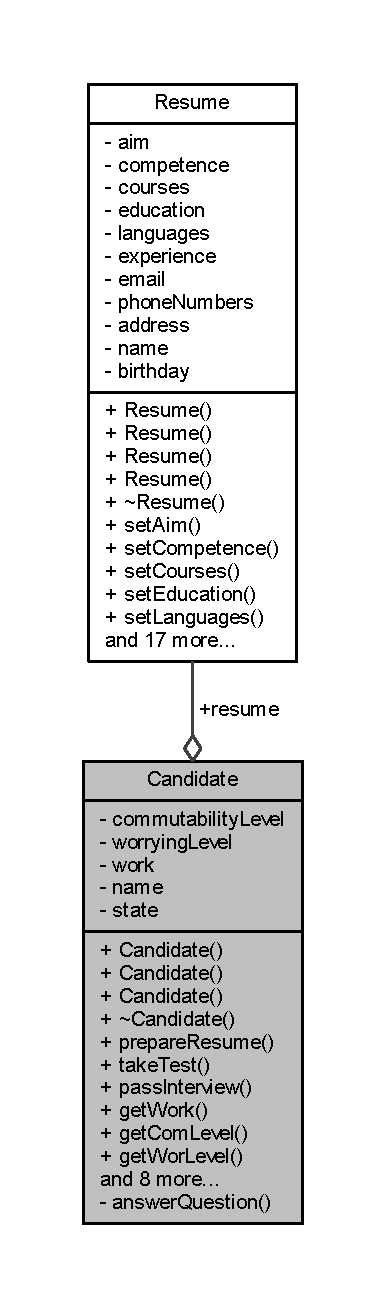
\includegraphics[height=550pt]{class_candidate__coll__graph}
\end{center}
\end{figure}
\subsection*{Public Member Functions}
\begin{DoxyCompactItemize}
\item 
\hyperlink{class_candidate_aa2747741fb662af5e8f3d01d1d1a43b6}{Candidate} ()
\item 
\hyperlink{class_candidate_a627ea8e00c8e5a4a6d4427a2ac41d41a}{Candidate} (int c\+Level, int w\+Level, bool \hyperlink{class_candidate_ab0a3583b677b47424e2da3f267a8036a}{work})
\item 
\hyperlink{class_candidate_a318c0f73f0e3091883c66ef970b3794e}{Candidate} (\hyperlink{class_candidate}{Candidate} \&s\+Candidate)
\item 
\hyperlink{class_candidate_a61ad4ae35e7a3ce5e5b91204b55c0b55}{$\sim$\+Candidate} ()
\item 
void \hyperlink{class_candidate_afee91575da03a495aad2f45f84ae341c}{prepare\+Resume} (void)
\item 
std\+::vector$<$ std\+::string $>$ \hyperlink{class_candidate_ab30f3859931c02d8cf69acb49a80c12e}{take\+Test} (std\+::vector$<$ std\+::string $>$ quetions)
\item 
void \hyperlink{class_candidate_ace55597a36842de9f9a44abf59be4eb2}{pass\+Interview} (void)
\item 
void \hyperlink{class_candidate_a50e84cbce900de9863aefb0f5f4a6f68}{get\+Work} (int time, std\+::vector$<$ std\+::string $>$ quetions, std\+::vector$<$ std\+::string $>$ $\ast$answ)
\item 
int \hyperlink{class_candidate_a12bd0777e1b813f1caa683832b28c8f6}{get\+Com\+Level} (void) const
\item 
int \hyperlink{class_candidate_aa6971bae134029ced1180e77bc3662ae}{get\+Wor\+Level} (void) const
\item 
std\+::string \hyperlink{class_candidate_a10f8f982418cc3db29c6f211a2b24ebf}{get\+Name} (void) const
\item 
std\+::string \hyperlink{class_candidate_a31fdda5e5a9cb8abbe3506b5a8bc33ab}{get\+State} (void) const
\item 
void \hyperlink{class_candidate_a936a7347b368ef38d994d4aecf4cee0c}{set\+Com\+Level} (int c)
\item 
void \hyperlink{class_candidate_ab526dc6819fcfb14821a7ba68c543d34}{set\+Wor\+Level} (int w)
\item 
void \hyperlink{class_candidate_ac500f9465747b144c7807b26987c2a3e}{set\+Work} (bool w)
\item 
void \hyperlink{class_candidate_a1fcf329a8244281d0ab8dd4100fc2c41}{set\+State} (std\+::string st)
\item 
bool \hyperlink{class_candidate_ae246e50a0bd6b9fc03a3579dbd178aad}{existence\+Of\+Work} (void)
\item 
bool \hyperlink{class_candidate_a8bfcd5a62801d4b6df95cf2ba29cf89d}{operator!} () const
\end{DoxyCompactItemize}
\subsection*{Public Attributes}
\begin{DoxyCompactItemize}
\item 
\hyperlink{class_resume}{Resume} \hyperlink{class_candidate_aa377897c9a9bdf566f7f1074f37d9ff1}{resume}
\end{DoxyCompactItemize}
\subsection*{Private Member Functions}
\begin{DoxyCompactItemize}
\item 
std\+::string \hyperlink{class_candidate_aa0d4d9afae45b7ce3a3808af2bfba228}{answer\+Question} (std\+::string dificult)
\end{DoxyCompactItemize}
\subsection*{Private Attributes}
\begin{DoxyCompactItemize}
\item 
int \hyperlink{class_candidate_a143f4a4644276e9a1914e12c4be8b986}{commutability\+Level}
\item 
int \hyperlink{class_candidate_a5c05cc634ba4472a0897d2e669f37963}{worrying\+Level}
\item 
bool \hyperlink{class_candidate_ab0a3583b677b47424e2da3f267a8036a}{work}
\item 
const std\+::string \hyperlink{class_candidate_ab3c913ca21b7c5239b48e551483bb808}{name}
\item 
std\+::string \hyperlink{class_candidate_a521dc0a66f6b111e5c70d64f6ecfbca5}{state}
\end{DoxyCompactItemize}
\subsection*{Friends}
\begin{DoxyCompactItemize}
\item 
std\+::ostream \& \hyperlink{class_candidate_ae89bdf092b73462b5a958aae6dbd35f0}{operator$<$$<$} (std\+::ostream \&stream, \hyperlink{class_candidate}{Candidate} candidate)
\end{DoxyCompactItemize}


\subsection{Constructor \& Destructor Documentation}
\hypertarget{class_candidate_aa2747741fb662af5e8f3d01d1d1a43b6}{}\label{class_candidate_aa2747741fb662af5e8f3d01d1d1a43b6} 
\index{Candidate@{Candidate}!Candidate@{Candidate}}
\index{Candidate@{Candidate}!Candidate@{Candidate}}
\subsubsection{\texorpdfstring{Candidate()}{Candidate()}\hspace{0.1cm}{\footnotesize\ttfamily [1/3]}}
{\footnotesize\ttfamily Candidate\+::\+Candidate (\begin{DoxyParamCaption}{ }\end{DoxyParamCaption})\hspace{0.3cm}{\ttfamily [inline]}}

\hypertarget{class_candidate_a627ea8e00c8e5a4a6d4427a2ac41d41a}{}\label{class_candidate_a627ea8e00c8e5a4a6d4427a2ac41d41a} 
\index{Candidate@{Candidate}!Candidate@{Candidate}}
\index{Candidate@{Candidate}!Candidate@{Candidate}}
\subsubsection{\texorpdfstring{Candidate()}{Candidate()}\hspace{0.1cm}{\footnotesize\ttfamily [2/3]}}
{\footnotesize\ttfamily Candidate\+::\+Candidate (\begin{DoxyParamCaption}\item[{int}]{c\+Level,  }\item[{int}]{w\+Level,  }\item[{bool}]{work }\end{DoxyParamCaption})\hspace{0.3cm}{\ttfamily [inline]}}

\hypertarget{class_candidate_a318c0f73f0e3091883c66ef970b3794e}{}\label{class_candidate_a318c0f73f0e3091883c66ef970b3794e} 
\index{Candidate@{Candidate}!Candidate@{Candidate}}
\index{Candidate@{Candidate}!Candidate@{Candidate}}
\subsubsection{\texorpdfstring{Candidate()}{Candidate()}\hspace{0.1cm}{\footnotesize\ttfamily [3/3]}}
{\footnotesize\ttfamily Candidate\+::\+Candidate (\begin{DoxyParamCaption}\item[{\hyperlink{class_candidate}{Candidate} \&}]{s\+Candidate }\end{DoxyParamCaption})\hspace{0.3cm}{\ttfamily [inline]}}

\hypertarget{class_candidate_a61ad4ae35e7a3ce5e5b91204b55c0b55}{}\label{class_candidate_a61ad4ae35e7a3ce5e5b91204b55c0b55} 
\index{Candidate@{Candidate}!````~Candidate@{$\sim$\+Candidate}}
\index{````~Candidate@{$\sim$\+Candidate}!Candidate@{Candidate}}
\subsubsection{\texorpdfstring{$\sim$\+Candidate()}{~Candidate()}}
{\footnotesize\ttfamily Candidate\+::$\sim$\+Candidate (\begin{DoxyParamCaption}{ }\end{DoxyParamCaption})\hspace{0.3cm}{\ttfamily [inline]}}

Here is the call graph for this function\+:
\nopagebreak
\begin{figure}[H]
\begin{center}
\leavevmode
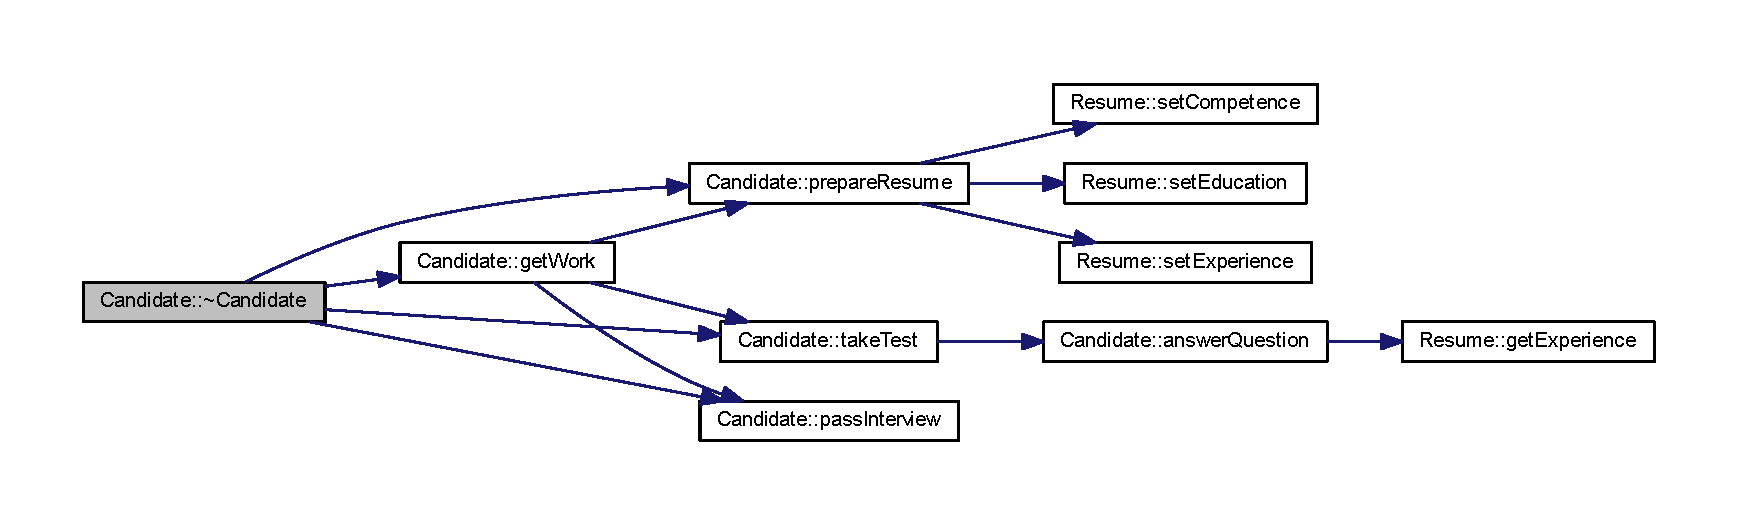
\includegraphics[width=350pt]{class_candidate_a61ad4ae35e7a3ce5e5b91204b55c0b55_cgraph}
\end{center}
\end{figure}


\subsection{Member Function Documentation}
\hypertarget{class_candidate_aa0d4d9afae45b7ce3a3808af2bfba228}{}\label{class_candidate_aa0d4d9afae45b7ce3a3808af2bfba228} 
\index{Candidate@{Candidate}!answer\+Question@{answer\+Question}}
\index{answer\+Question@{answer\+Question}!Candidate@{Candidate}}
\subsubsection{\texorpdfstring{answer\+Question()}{answerQuestion()}}
{\footnotesize\ttfamily std\+::string Candidate\+::answer\+Question (\begin{DoxyParamCaption}\item[{std\+::string}]{dificult }\end{DoxyParamCaption})\hspace{0.3cm}{\ttfamily [private]}}

Here is the call graph for this function\+:
\nopagebreak
\begin{figure}[H]
\begin{center}
\leavevmode
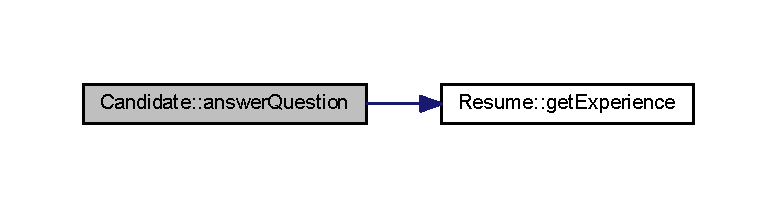
\includegraphics[width=350pt]{class_candidate_aa0d4d9afae45b7ce3a3808af2bfba228_cgraph}
\end{center}
\end{figure}
Here is the caller graph for this function\+:
\nopagebreak
\begin{figure}[H]
\begin{center}
\leavevmode
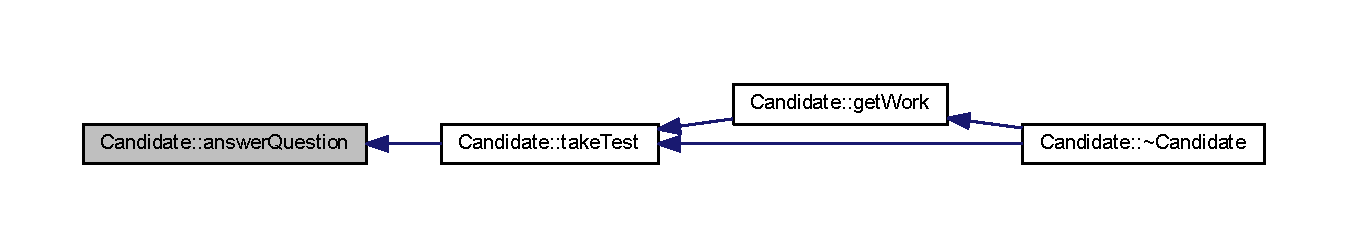
\includegraphics[width=350pt]{class_candidate_aa0d4d9afae45b7ce3a3808af2bfba228_icgraph}
\end{center}
\end{figure}
\hypertarget{class_candidate_ae246e50a0bd6b9fc03a3579dbd178aad}{}\label{class_candidate_ae246e50a0bd6b9fc03a3579dbd178aad} 
\index{Candidate@{Candidate}!existence\+Of\+Work@{existence\+Of\+Work}}
\index{existence\+Of\+Work@{existence\+Of\+Work}!Candidate@{Candidate}}
\subsubsection{\texorpdfstring{existence\+Of\+Work()}{existenceOfWork()}}
{\footnotesize\ttfamily bool Candidate\+::existence\+Of\+Work (\begin{DoxyParamCaption}\item[{void}]{ }\end{DoxyParamCaption})\hspace{0.3cm}{\ttfamily [inline]}}

\hypertarget{class_candidate_a12bd0777e1b813f1caa683832b28c8f6}{}\label{class_candidate_a12bd0777e1b813f1caa683832b28c8f6} 
\index{Candidate@{Candidate}!get\+Com\+Level@{get\+Com\+Level}}
\index{get\+Com\+Level@{get\+Com\+Level}!Candidate@{Candidate}}
\subsubsection{\texorpdfstring{get\+Com\+Level()}{getComLevel()}}
{\footnotesize\ttfamily int Candidate\+::get\+Com\+Level (\begin{DoxyParamCaption}\item[{void}]{ }\end{DoxyParamCaption}) const\hspace{0.3cm}{\ttfamily [inline]}}

\hypertarget{class_candidate_a10f8f982418cc3db29c6f211a2b24ebf}{}\label{class_candidate_a10f8f982418cc3db29c6f211a2b24ebf} 
\index{Candidate@{Candidate}!get\+Name@{get\+Name}}
\index{get\+Name@{get\+Name}!Candidate@{Candidate}}
\subsubsection{\texorpdfstring{get\+Name()}{getName()}}
{\footnotesize\ttfamily std\+::string Candidate\+::get\+Name (\begin{DoxyParamCaption}\item[{void}]{ }\end{DoxyParamCaption}) const\hspace{0.3cm}{\ttfamily [inline]}}

Here is the caller graph for this function\+:
\nopagebreak
\begin{figure}[H]
\begin{center}
\leavevmode
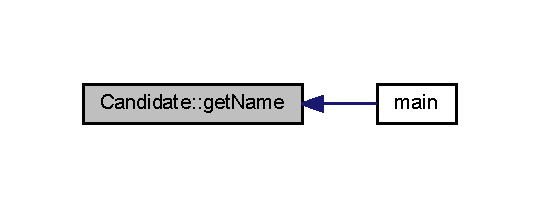
\includegraphics[width=259pt]{class_candidate_a10f8f982418cc3db29c6f211a2b24ebf_icgraph}
\end{center}
\end{figure}
\hypertarget{class_candidate_a31fdda5e5a9cb8abbe3506b5a8bc33ab}{}\label{class_candidate_a31fdda5e5a9cb8abbe3506b5a8bc33ab} 
\index{Candidate@{Candidate}!get\+State@{get\+State}}
\index{get\+State@{get\+State}!Candidate@{Candidate}}
\subsubsection{\texorpdfstring{get\+State()}{getState()}}
{\footnotesize\ttfamily std\+::string Candidate\+::get\+State (\begin{DoxyParamCaption}\item[{void}]{ }\end{DoxyParamCaption}) const\hspace{0.3cm}{\ttfamily [inline]}}

\hypertarget{class_candidate_a50e84cbce900de9863aefb0f5f4a6f68}{}\label{class_candidate_a50e84cbce900de9863aefb0f5f4a6f68} 
\index{Candidate@{Candidate}!get\+Work@{get\+Work}}
\index{get\+Work@{get\+Work}!Candidate@{Candidate}}
\subsubsection{\texorpdfstring{get\+Work()}{getWork()}}
{\footnotesize\ttfamily void Candidate\+::get\+Work (\begin{DoxyParamCaption}\item[{int}]{time,  }\item[{std\+::vector$<$ std\+::string $>$}]{quetions,  }\item[{std\+::vector$<$ std\+::string $>$ $\ast$}]{answ }\end{DoxyParamCaption})}

Here is the call graph for this function\+:
\nopagebreak
\begin{figure}[H]
\begin{center}
\leavevmode
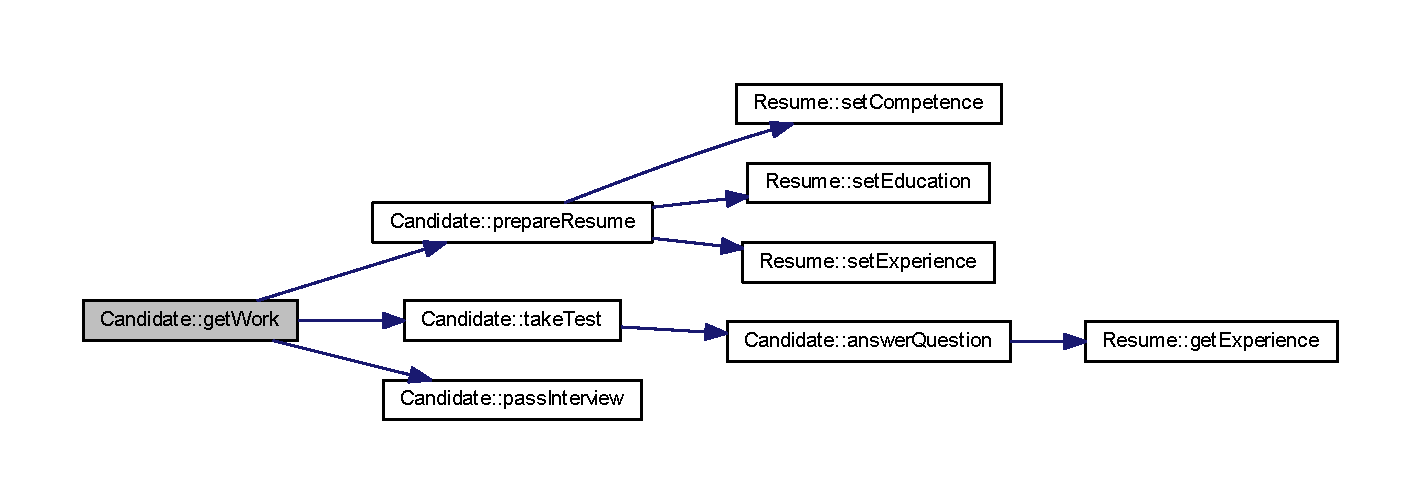
\includegraphics[width=350pt]{class_candidate_a50e84cbce900de9863aefb0f5f4a6f68_cgraph}
\end{center}
\end{figure}
Here is the caller graph for this function\+:
\nopagebreak
\begin{figure}[H]
\begin{center}
\leavevmode
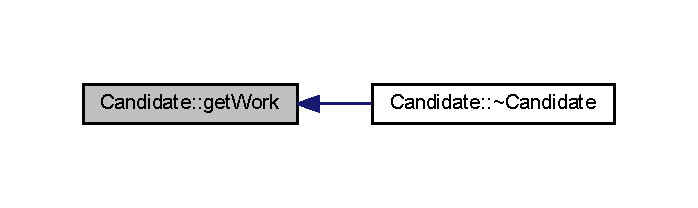
\includegraphics[width=335pt]{class_candidate_a50e84cbce900de9863aefb0f5f4a6f68_icgraph}
\end{center}
\end{figure}
\hypertarget{class_candidate_aa6971bae134029ced1180e77bc3662ae}{}\label{class_candidate_aa6971bae134029ced1180e77bc3662ae} 
\index{Candidate@{Candidate}!get\+Wor\+Level@{get\+Wor\+Level}}
\index{get\+Wor\+Level@{get\+Wor\+Level}!Candidate@{Candidate}}
\subsubsection{\texorpdfstring{get\+Wor\+Level()}{getWorLevel()}}
{\footnotesize\ttfamily int Candidate\+::get\+Wor\+Level (\begin{DoxyParamCaption}\item[{void}]{ }\end{DoxyParamCaption}) const\hspace{0.3cm}{\ttfamily [inline]}}

\hypertarget{class_candidate_a8bfcd5a62801d4b6df95cf2ba29cf89d}{}\label{class_candidate_a8bfcd5a62801d4b6df95cf2ba29cf89d} 
\index{Candidate@{Candidate}!operator"!@{operator"!}}
\index{operator"!@{operator"!}!Candidate@{Candidate}}
\subsubsection{\texorpdfstring{operator"!()}{operator!()}}
{\footnotesize\ttfamily bool Candidate\+::operator! (\begin{DoxyParamCaption}{ }\end{DoxyParamCaption}) const\hspace{0.3cm}{\ttfamily [inline]}}

\hypertarget{class_candidate_ace55597a36842de9f9a44abf59be4eb2}{}\label{class_candidate_ace55597a36842de9f9a44abf59be4eb2} 
\index{Candidate@{Candidate}!pass\+Interview@{pass\+Interview}}
\index{pass\+Interview@{pass\+Interview}!Candidate@{Candidate}}
\subsubsection{\texorpdfstring{pass\+Interview()}{passInterview()}}
{\footnotesize\ttfamily void Candidate\+::pass\+Interview (\begin{DoxyParamCaption}\item[{void}]{ }\end{DoxyParamCaption})}

Here is the caller graph for this function\+:
\nopagebreak
\begin{figure}[H]
\begin{center}
\leavevmode
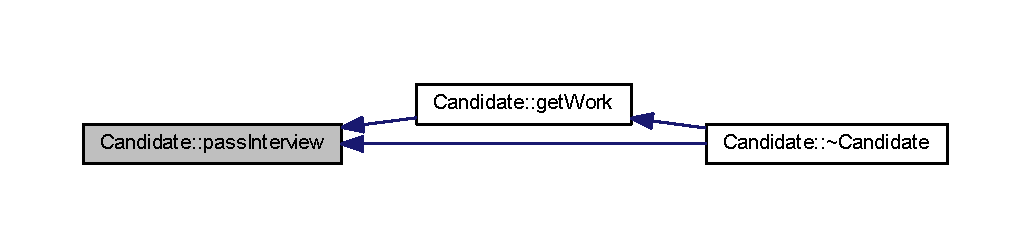
\includegraphics[width=350pt]{class_candidate_ace55597a36842de9f9a44abf59be4eb2_icgraph}
\end{center}
\end{figure}
\hypertarget{class_candidate_afee91575da03a495aad2f45f84ae341c}{}\label{class_candidate_afee91575da03a495aad2f45f84ae341c} 
\index{Candidate@{Candidate}!prepare\+Resume@{prepare\+Resume}}
\index{prepare\+Resume@{prepare\+Resume}!Candidate@{Candidate}}
\subsubsection{\texorpdfstring{prepare\+Resume()}{prepareResume()}}
{\footnotesize\ttfamily void Candidate\+::prepare\+Resume (\begin{DoxyParamCaption}\item[{void}]{ }\end{DoxyParamCaption})}

Here is the call graph for this function\+:
\nopagebreak
\begin{figure}[H]
\begin{center}
\leavevmode
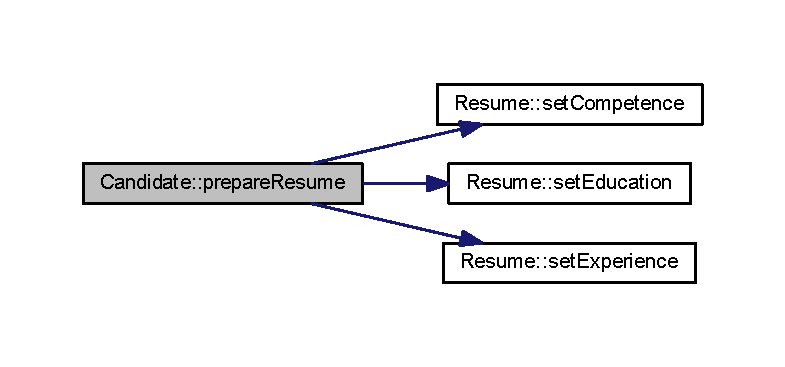
\includegraphics[width=350pt]{class_candidate_afee91575da03a495aad2f45f84ae341c_cgraph}
\end{center}
\end{figure}
Here is the caller graph for this function\+:
\nopagebreak
\begin{figure}[H]
\begin{center}
\leavevmode
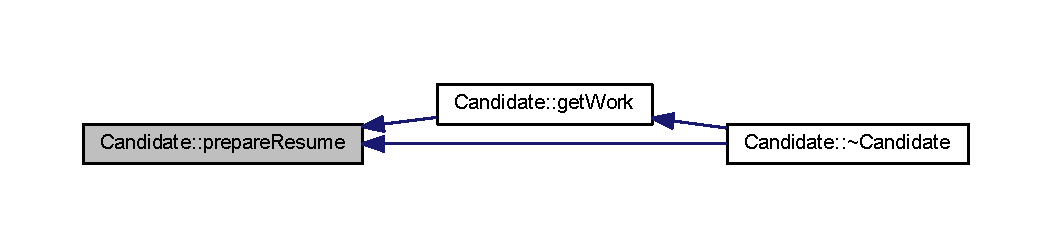
\includegraphics[width=350pt]{class_candidate_afee91575da03a495aad2f45f84ae341c_icgraph}
\end{center}
\end{figure}
\hypertarget{class_candidate_a936a7347b368ef38d994d4aecf4cee0c}{}\label{class_candidate_a936a7347b368ef38d994d4aecf4cee0c} 
\index{Candidate@{Candidate}!set\+Com\+Level@{set\+Com\+Level}}
\index{set\+Com\+Level@{set\+Com\+Level}!Candidate@{Candidate}}
\subsubsection{\texorpdfstring{set\+Com\+Level()}{setComLevel()}}
{\footnotesize\ttfamily void Candidate\+::set\+Com\+Level (\begin{DoxyParamCaption}\item[{int}]{c }\end{DoxyParamCaption})\hspace{0.3cm}{\ttfamily [inline]}}

\hypertarget{class_candidate_a1fcf329a8244281d0ab8dd4100fc2c41}{}\label{class_candidate_a1fcf329a8244281d0ab8dd4100fc2c41} 
\index{Candidate@{Candidate}!set\+State@{set\+State}}
\index{set\+State@{set\+State}!Candidate@{Candidate}}
\subsubsection{\texorpdfstring{set\+State()}{setState()}}
{\footnotesize\ttfamily void Candidate\+::set\+State (\begin{DoxyParamCaption}\item[{std\+::string}]{st }\end{DoxyParamCaption})\hspace{0.3cm}{\ttfamily [inline]}}

\hypertarget{class_candidate_ac500f9465747b144c7807b26987c2a3e}{}\label{class_candidate_ac500f9465747b144c7807b26987c2a3e} 
\index{Candidate@{Candidate}!set\+Work@{set\+Work}}
\index{set\+Work@{set\+Work}!Candidate@{Candidate}}
\subsubsection{\texorpdfstring{set\+Work()}{setWork()}}
{\footnotesize\ttfamily void Candidate\+::set\+Work (\begin{DoxyParamCaption}\item[{bool}]{w }\end{DoxyParamCaption})\hspace{0.3cm}{\ttfamily [inline]}}

\hypertarget{class_candidate_ab526dc6819fcfb14821a7ba68c543d34}{}\label{class_candidate_ab526dc6819fcfb14821a7ba68c543d34} 
\index{Candidate@{Candidate}!set\+Wor\+Level@{set\+Wor\+Level}}
\index{set\+Wor\+Level@{set\+Wor\+Level}!Candidate@{Candidate}}
\subsubsection{\texorpdfstring{set\+Wor\+Level()}{setWorLevel()}}
{\footnotesize\ttfamily void Candidate\+::set\+Wor\+Level (\begin{DoxyParamCaption}\item[{int}]{w }\end{DoxyParamCaption})\hspace{0.3cm}{\ttfamily [inline]}}

\hypertarget{class_candidate_ab30f3859931c02d8cf69acb49a80c12e}{}\label{class_candidate_ab30f3859931c02d8cf69acb49a80c12e} 
\index{Candidate@{Candidate}!take\+Test@{take\+Test}}
\index{take\+Test@{take\+Test}!Candidate@{Candidate}}
\subsubsection{\texorpdfstring{take\+Test()}{takeTest()}}
{\footnotesize\ttfamily std\+::vector$<$ std\+::string $>$ Candidate\+::take\+Test (\begin{DoxyParamCaption}\item[{std\+::vector$<$ std\+::string $>$}]{quetions }\end{DoxyParamCaption})}

Here is the call graph for this function\+:
\nopagebreak
\begin{figure}[H]
\begin{center}
\leavevmode
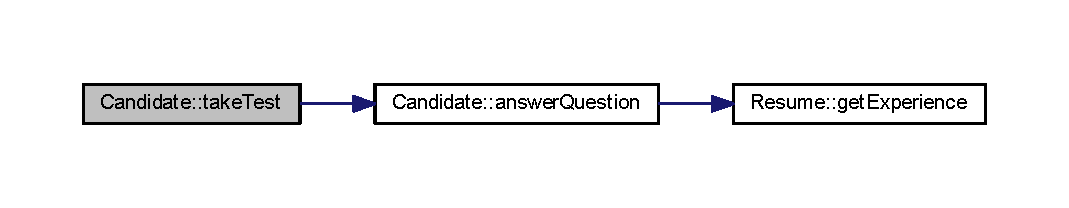
\includegraphics[width=350pt]{class_candidate_ab30f3859931c02d8cf69acb49a80c12e_cgraph}
\end{center}
\end{figure}
Here is the caller graph for this function\+:
\nopagebreak
\begin{figure}[H]
\begin{center}
\leavevmode
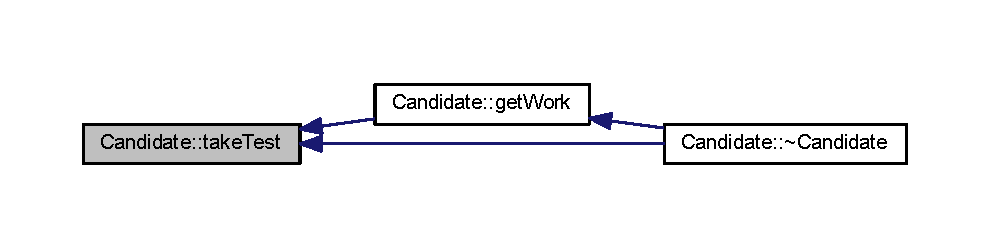
\includegraphics[width=350pt]{class_candidate_ab30f3859931c02d8cf69acb49a80c12e_icgraph}
\end{center}
\end{figure}


\subsection{Friends And Related Function Documentation}
\hypertarget{class_candidate_ae89bdf092b73462b5a958aae6dbd35f0}{}\label{class_candidate_ae89bdf092b73462b5a958aae6dbd35f0} 
\index{Candidate@{Candidate}!operator$<$$<$@{operator$<$$<$}}
\index{operator$<$$<$@{operator$<$$<$}!Candidate@{Candidate}}
\subsubsection{\texorpdfstring{operator$<$$<$}{operator<<}}
{\footnotesize\ttfamily std\+::ostream\& operator$<$$<$ (\begin{DoxyParamCaption}\item[{std\+::ostream \&}]{stream,  }\item[{\hyperlink{class_candidate}{Candidate}}]{candidate }\end{DoxyParamCaption})\hspace{0.3cm}{\ttfamily [friend]}}



\subsection{Member Data Documentation}
\hypertarget{class_candidate_a143f4a4644276e9a1914e12c4be8b986}{}\label{class_candidate_a143f4a4644276e9a1914e12c4be8b986} 
\index{Candidate@{Candidate}!commutability\+Level@{commutability\+Level}}
\index{commutability\+Level@{commutability\+Level}!Candidate@{Candidate}}
\subsubsection{\texorpdfstring{commutability\+Level}{commutabilityLevel}}
{\footnotesize\ttfamily int Candidate\+::commutability\+Level\hspace{0.3cm}{\ttfamily [private]}}

\hypertarget{class_candidate_ab3c913ca21b7c5239b48e551483bb808}{}\label{class_candidate_ab3c913ca21b7c5239b48e551483bb808} 
\index{Candidate@{Candidate}!name@{name}}
\index{name@{name}!Candidate@{Candidate}}
\subsubsection{\texorpdfstring{name}{name}}
{\footnotesize\ttfamily const std\+::string Candidate\+::name\hspace{0.3cm}{\ttfamily [private]}}

\hypertarget{class_candidate_aa377897c9a9bdf566f7f1074f37d9ff1}{}\label{class_candidate_aa377897c9a9bdf566f7f1074f37d9ff1} 
\index{Candidate@{Candidate}!resume@{resume}}
\index{resume@{resume}!Candidate@{Candidate}}
\subsubsection{\texorpdfstring{resume}{resume}}
{\footnotesize\ttfamily \hyperlink{class_resume}{Resume} Candidate\+::resume}

\hypertarget{class_candidate_a521dc0a66f6b111e5c70d64f6ecfbca5}{}\label{class_candidate_a521dc0a66f6b111e5c70d64f6ecfbca5} 
\index{Candidate@{Candidate}!state@{state}}
\index{state@{state}!Candidate@{Candidate}}
\subsubsection{\texorpdfstring{state}{state}}
{\footnotesize\ttfamily std\+::string Candidate\+::state\hspace{0.3cm}{\ttfamily [private]}}

\hypertarget{class_candidate_ab0a3583b677b47424e2da3f267a8036a}{}\label{class_candidate_ab0a3583b677b47424e2da3f267a8036a} 
\index{Candidate@{Candidate}!work@{work}}
\index{work@{work}!Candidate@{Candidate}}
\subsubsection{\texorpdfstring{work}{work}}
{\footnotesize\ttfamily bool Candidate\+::work\hspace{0.3cm}{\ttfamily [private]}}

\hypertarget{class_candidate_a5c05cc634ba4472a0897d2e669f37963}{}\label{class_candidate_a5c05cc634ba4472a0897d2e669f37963} 
\index{Candidate@{Candidate}!worrying\+Level@{worrying\+Level}}
\index{worrying\+Level@{worrying\+Level}!Candidate@{Candidate}}
\subsubsection{\texorpdfstring{worrying\+Level}{worryingLevel}}
{\footnotesize\ttfamily int Candidate\+::worrying\+Level\hspace{0.3cm}{\ttfamily [private]}}



The documentation for this class was generated from the following files\+:\begin{DoxyCompactItemize}
\item 
\hyperlink{_candidate_8h}{Candidate.\+h}\item 
\hyperlink{_candidate_8cpp}{Candidate.\+cpp}\end{DoxyCompactItemize}

\hypertarget{class_error}{}\section{Error Class Reference}
\label{class_error}\index{Error@{Error}}


{\ttfamily \#include $<$Error.\+h$>$}



Collaboration diagram for Error\+:
\nopagebreak
\begin{figure}[H]
\begin{center}
\leavevmode
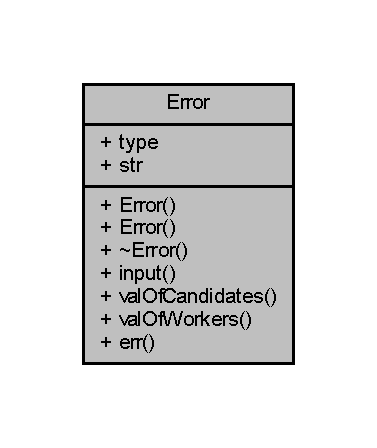
\includegraphics[width=181pt]{class_error__coll__graph}
\end{center}
\end{figure}
\subsection*{Public Member Functions}
\begin{DoxyCompactItemize}
\item 
\hyperlink{class_error_aca339d00ad8481fb4c184f0ece42698b}{Error} ()
\item 
\hyperlink{class_error_a9e6a79d4d774de29af7a7ea7fe3f8c7b}{Error} (int t, std\+::string $\ast$\hyperlink{class_error_adef2e029304986e6210e7f81f0dca074}{str})
\item 
\hyperlink{class_error_a1a45d42a3a035d510333cdfeb36a0e93}{$\sim$\+Error} ()
\item 
void \hyperlink{class_error_a9f20c7656a23e4f4cf1fa600ced37421}{input} (std\+::string $\ast$)
\item 
void \hyperlink{class_error_a35ab6ad1cad16467c4817cdc8e3ebaea}{val\+Of\+Candidates} ()
\item 
void \hyperlink{class_error_a5d7c6b97cda36f85a426dd2032c242d3}{val\+Of\+Workers} ()
\item 
void \hyperlink{class_error_a047207c59d0f2bedd19256e011abb80e}{err} (std\+::string $\ast$)
\end{DoxyCompactItemize}
\subsection*{Public Attributes}
\begin{DoxyCompactItemize}
\item 
int \hyperlink{class_error_a87ec3b472513bcf651c0facbd9926c7c}{type}
\item 
std\+::string $\ast$ \hyperlink{class_error_adef2e029304986e6210e7f81f0dca074}{str}
\end{DoxyCompactItemize}


\subsection{Constructor \& Destructor Documentation}
\hypertarget{class_error_aca339d00ad8481fb4c184f0ece42698b}{}\label{class_error_aca339d00ad8481fb4c184f0ece42698b} 
\index{Error@{Error}!Error@{Error}}
\index{Error@{Error}!Error@{Error}}
\subsubsection{\texorpdfstring{Error()}{Error()}\hspace{0.1cm}{\footnotesize\ttfamily [1/2]}}
{\footnotesize\ttfamily Error\+::\+Error (\begin{DoxyParamCaption}{ }\end{DoxyParamCaption})\hspace{0.3cm}{\ttfamily [inline]}}

\hypertarget{class_error_a9e6a79d4d774de29af7a7ea7fe3f8c7b}{}\label{class_error_a9e6a79d4d774de29af7a7ea7fe3f8c7b} 
\index{Error@{Error}!Error@{Error}}
\index{Error@{Error}!Error@{Error}}
\subsubsection{\texorpdfstring{Error()}{Error()}\hspace{0.1cm}{\footnotesize\ttfamily [2/2]}}
{\footnotesize\ttfamily Error\+::\+Error (\begin{DoxyParamCaption}\item[{int}]{t,  }\item[{std\+::string $\ast$}]{str }\end{DoxyParamCaption})\hspace{0.3cm}{\ttfamily [inline]}}

\hypertarget{class_error_a1a45d42a3a035d510333cdfeb36a0e93}{}\label{class_error_a1a45d42a3a035d510333cdfeb36a0e93} 
\index{Error@{Error}!````~Error@{$\sim$\+Error}}
\index{````~Error@{$\sim$\+Error}!Error@{Error}}
\subsubsection{\texorpdfstring{$\sim$\+Error()}{~Error()}}
{\footnotesize\ttfamily Error\+::$\sim$\+Error (\begin{DoxyParamCaption}{ }\end{DoxyParamCaption})\hspace{0.3cm}{\ttfamily [inline]}}

Here is the call graph for this function\+:
\nopagebreak
\begin{figure}[H]
\begin{center}
\leavevmode
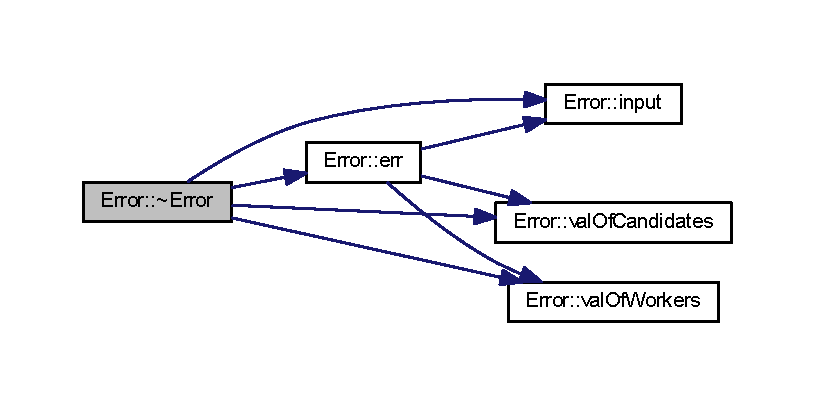
\includegraphics[width=350pt]{class_error_a1a45d42a3a035d510333cdfeb36a0e93_cgraph}
\end{center}
\end{figure}


\subsection{Member Function Documentation}
\hypertarget{class_error_a047207c59d0f2bedd19256e011abb80e}{}\label{class_error_a047207c59d0f2bedd19256e011abb80e} 
\index{Error@{Error}!err@{err}}
\index{err@{err}!Error@{Error}}
\subsubsection{\texorpdfstring{err()}{err()}}
{\footnotesize\ttfamily void Error\+::err (\begin{DoxyParamCaption}\item[{std\+::string $\ast$}]{str }\end{DoxyParamCaption})}

Here is the call graph for this function\+:
\nopagebreak
\begin{figure}[H]
\begin{center}
\leavevmode
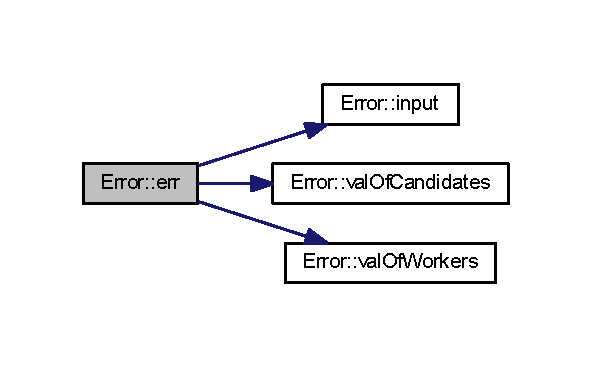
\includegraphics[width=284pt]{class_error_a047207c59d0f2bedd19256e011abb80e_cgraph}
\end{center}
\end{figure}
Here is the caller graph for this function\+:
\nopagebreak
\begin{figure}[H]
\begin{center}
\leavevmode
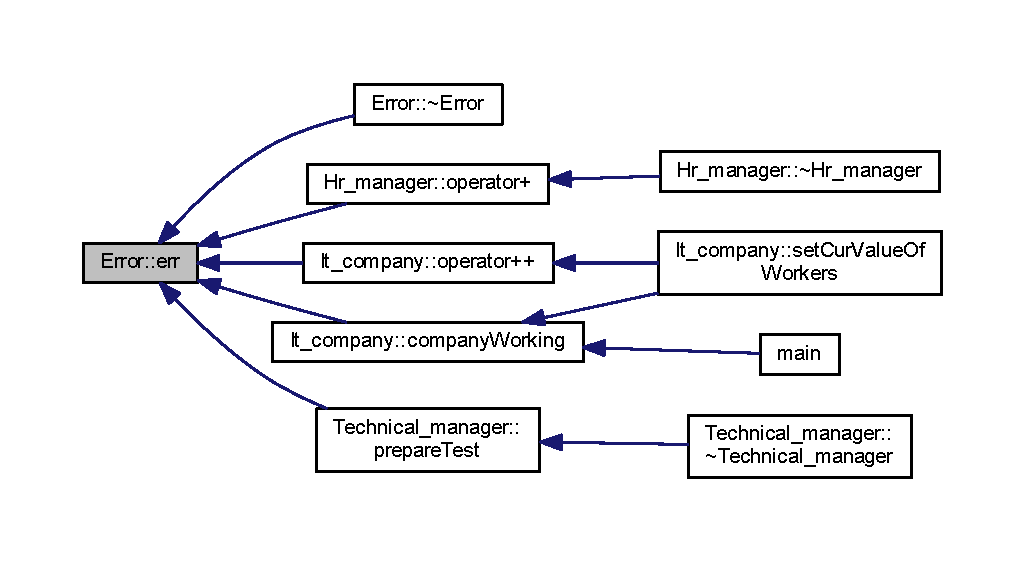
\includegraphics[width=350pt]{class_error_a047207c59d0f2bedd19256e011abb80e_icgraph}
\end{center}
\end{figure}
\hypertarget{class_error_a9f20c7656a23e4f4cf1fa600ced37421}{}\label{class_error_a9f20c7656a23e4f4cf1fa600ced37421} 
\index{Error@{Error}!input@{input}}
\index{input@{input}!Error@{Error}}
\subsubsection{\texorpdfstring{input()}{input()}}
{\footnotesize\ttfamily void Error\+::input (\begin{DoxyParamCaption}\item[{std\+::string $\ast$}]{str }\end{DoxyParamCaption})}

Here is the caller graph for this function\+:
\nopagebreak
\begin{figure}[H]
\begin{center}
\leavevmode
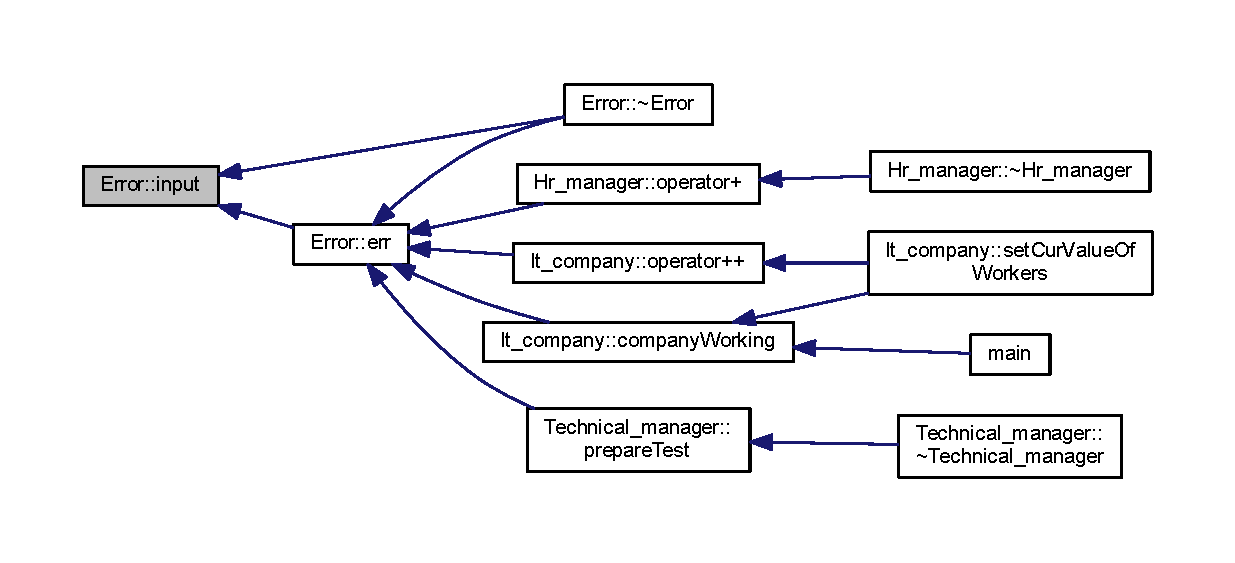
\includegraphics[width=350pt]{class_error_a9f20c7656a23e4f4cf1fa600ced37421_icgraph}
\end{center}
\end{figure}
\hypertarget{class_error_a35ab6ad1cad16467c4817cdc8e3ebaea}{}\label{class_error_a35ab6ad1cad16467c4817cdc8e3ebaea} 
\index{Error@{Error}!val\+Of\+Candidates@{val\+Of\+Candidates}}
\index{val\+Of\+Candidates@{val\+Of\+Candidates}!Error@{Error}}
\subsubsection{\texorpdfstring{val\+Of\+Candidates()}{valOfCandidates()}}
{\footnotesize\ttfamily void Error\+::val\+Of\+Candidates (\begin{DoxyParamCaption}{ }\end{DoxyParamCaption})}

Here is the caller graph for this function\+:
\nopagebreak
\begin{figure}[H]
\begin{center}
\leavevmode
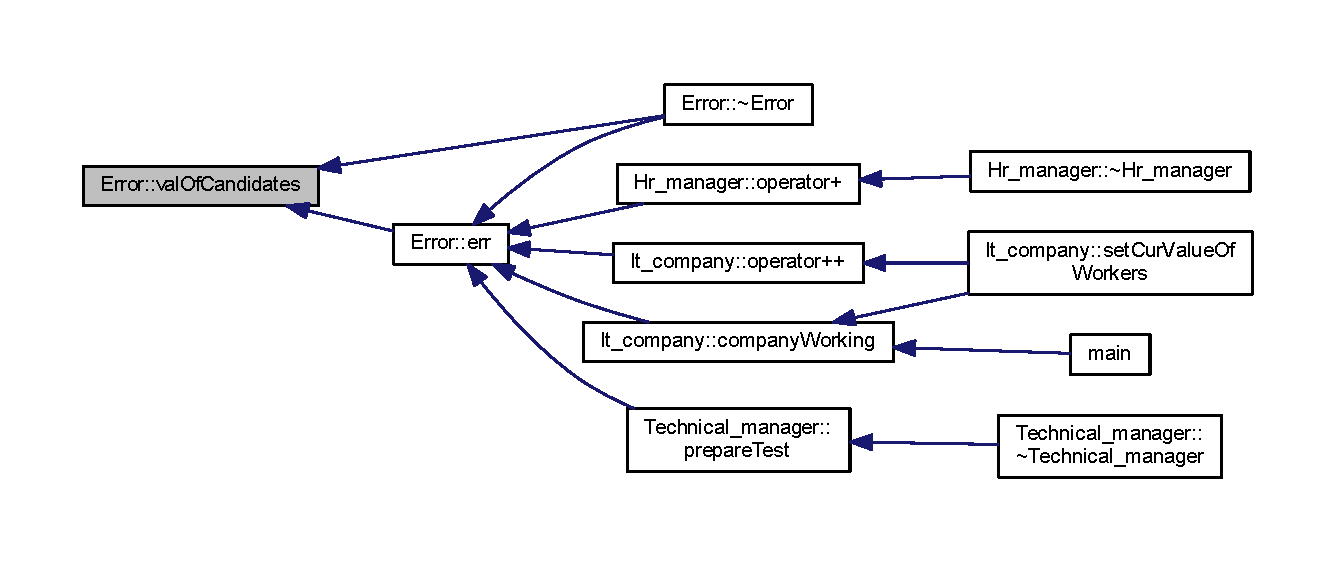
\includegraphics[width=350pt]{class_error_a35ab6ad1cad16467c4817cdc8e3ebaea_icgraph}
\end{center}
\end{figure}
\hypertarget{class_error_a5d7c6b97cda36f85a426dd2032c242d3}{}\label{class_error_a5d7c6b97cda36f85a426dd2032c242d3} 
\index{Error@{Error}!val\+Of\+Workers@{val\+Of\+Workers}}
\index{val\+Of\+Workers@{val\+Of\+Workers}!Error@{Error}}
\subsubsection{\texorpdfstring{val\+Of\+Workers()}{valOfWorkers()}}
{\footnotesize\ttfamily void Error\+::val\+Of\+Workers (\begin{DoxyParamCaption}{ }\end{DoxyParamCaption})}

Here is the caller graph for this function\+:
\nopagebreak
\begin{figure}[H]
\begin{center}
\leavevmode
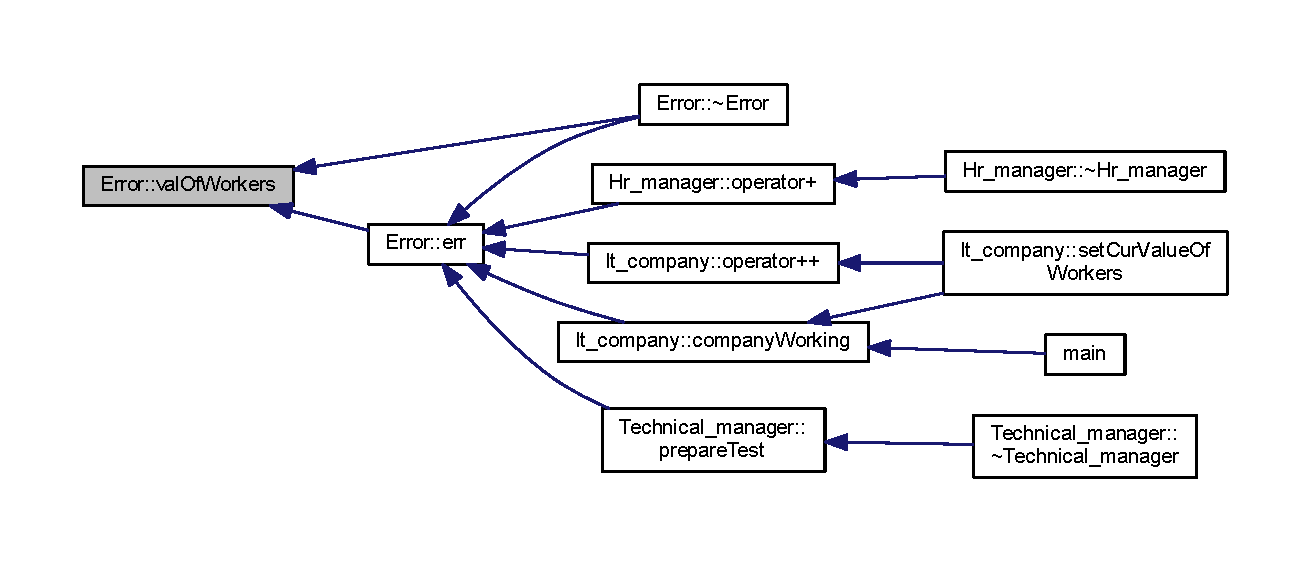
\includegraphics[width=350pt]{class_error_a5d7c6b97cda36f85a426dd2032c242d3_icgraph}
\end{center}
\end{figure}


\subsection{Member Data Documentation}
\hypertarget{class_error_adef2e029304986e6210e7f81f0dca074}{}\label{class_error_adef2e029304986e6210e7f81f0dca074} 
\index{Error@{Error}!str@{str}}
\index{str@{str}!Error@{Error}}
\subsubsection{\texorpdfstring{str}{str}}
{\footnotesize\ttfamily std\+::string$\ast$ Error\+::str}

\hypertarget{class_error_a87ec3b472513bcf651c0facbd9926c7c}{}\label{class_error_a87ec3b472513bcf651c0facbd9926c7c} 
\index{Error@{Error}!type@{type}}
\index{type@{type}!Error@{Error}}
\subsubsection{\texorpdfstring{type}{type}}
{\footnotesize\ttfamily int Error\+::type}



The documentation for this class was generated from the following files\+:\begin{DoxyCompactItemize}
\item 
\hyperlink{_error_8h}{Error.\+h}\item 
\hyperlink{_error_8cpp}{Error.\+cpp}\end{DoxyCompactItemize}

\hypertarget{class_hr__manager}{}\section{Hr\+\_\+manager Class Reference}
\label{class_hr__manager}\index{Hr\+\_\+manager@{Hr\+\_\+manager}}


{\ttfamily \#include $<$Hr\+\_\+manager.\+h$>$}



Inheritance diagram for Hr\+\_\+manager\+:
\nopagebreak
\begin{figure}[H]
\begin{center}
\leavevmode
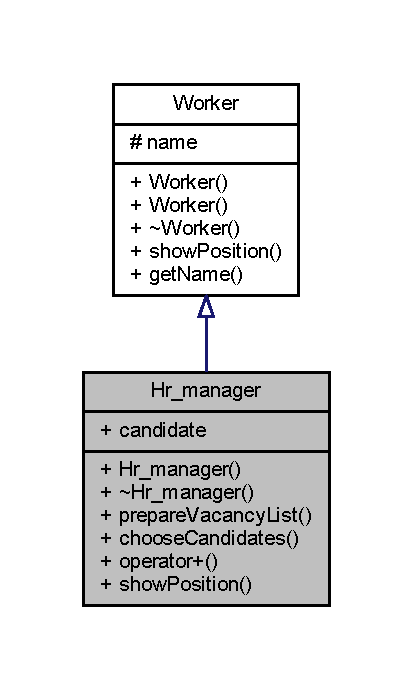
\includegraphics[width=198pt]{class_hr__manager__inherit__graph}
\end{center}
\end{figure}


Collaboration diagram for Hr\+\_\+manager\+:
\nopagebreak
\begin{figure}[H]
\begin{center}
\leavevmode
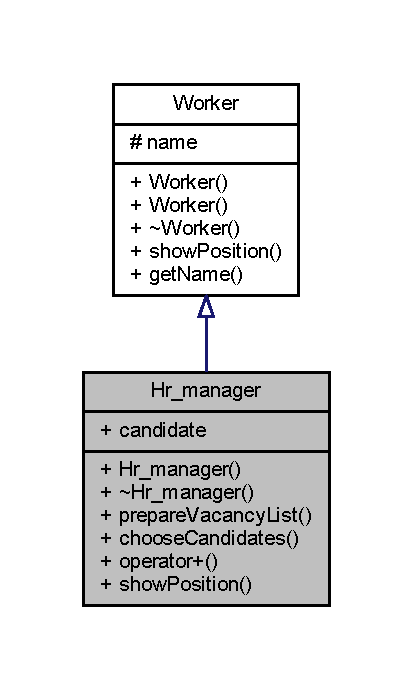
\includegraphics[width=198pt]{class_hr__manager__coll__graph}
\end{center}
\end{figure}
\subsection*{Public Member Functions}
\begin{DoxyCompactItemize}
\item 
\hyperlink{class_hr__manager_a887008e77b1f49947fc52ace7b36212b}{Hr\+\_\+manager} ()
\item 
\hyperlink{class_hr__manager_a6713d753a80cf4346da53d52876e751f}{$\sim$\+Hr\+\_\+manager} ()
\item 
std\+::vector$<$ std\+::string $>$ \hyperlink{class_hr__manager_a579ebdb8579aace02b9c2d2f29051c77}{prepare\+Vacancy\+List} (int max, int cur)
\item 
void \hyperlink{class_hr__manager_ad172002747343f207758c2ea76d6e480}{choose\+Candidates} (std\+::vector$<$ std\+::string $>$ list)
\item 
\hyperlink{class_hr__manager}{Hr\+\_\+manager} \hyperlink{class_hr__manager_a3315b88815233ab95cd924280086d8a9}{operator+} (\hyperlink{class_candidate}{Candidate} \&right)
\item 
void \hyperlink{class_hr__manager_a760e884af11ec93a1dbf3769cdf34adf}{show\+Position} ()
\end{DoxyCompactItemize}
\subsection*{Public Attributes}
\begin{DoxyCompactItemize}
\item 
std\+::vector$<$ \hyperlink{class_candidate}{Candidate} $\ast$ $>$ \hyperlink{class_hr__manager_a4f136a7a1ad3c57b8463b3e627a5c5f5}{candidate}
\end{DoxyCompactItemize}
\subsection*{Friends}
\begin{DoxyCompactItemize}
\item 
std\+::ostream \& \hyperlink{class_hr__manager_a954d2b0eb5d6bd979593a3d4018f52c5}{operator$<$$<$} (std\+::ostream \&stream, \hyperlink{class_hr__manager}{Hr\+\_\+manager} hrmanager)
\end{DoxyCompactItemize}
\subsection*{Additional Inherited Members}


\subsection{Constructor \& Destructor Documentation}
\hypertarget{class_hr__manager_a887008e77b1f49947fc52ace7b36212b}{}\label{class_hr__manager_a887008e77b1f49947fc52ace7b36212b} 
\index{Hr\+\_\+manager@{Hr\+\_\+manager}!Hr\+\_\+manager@{Hr\+\_\+manager}}
\index{Hr\+\_\+manager@{Hr\+\_\+manager}!Hr\+\_\+manager@{Hr\+\_\+manager}}
\subsubsection{\texorpdfstring{Hr\+\_\+manager()}{Hr\_manager()}}
{\footnotesize\ttfamily Hr\+\_\+manager\+::\+Hr\+\_\+manager (\begin{DoxyParamCaption}{ }\end{DoxyParamCaption})\hspace{0.3cm}{\ttfamily [inline]}}

\hypertarget{class_hr__manager_a6713d753a80cf4346da53d52876e751f}{}\label{class_hr__manager_a6713d753a80cf4346da53d52876e751f} 
\index{Hr\+\_\+manager@{Hr\+\_\+manager}!````~Hr\+\_\+manager@{$\sim$\+Hr\+\_\+manager}}
\index{````~Hr\+\_\+manager@{$\sim$\+Hr\+\_\+manager}!Hr\+\_\+manager@{Hr\+\_\+manager}}
\subsubsection{\texorpdfstring{$\sim$\+Hr\+\_\+manager()}{~Hr\_manager()}}
{\footnotesize\ttfamily Hr\+\_\+manager\+::$\sim$\+Hr\+\_\+manager (\begin{DoxyParamCaption}{ }\end{DoxyParamCaption})\hspace{0.3cm}{\ttfamily [inline]}}

Here is the call graph for this function\+:
\nopagebreak
\begin{figure}[H]
\begin{center}
\leavevmode
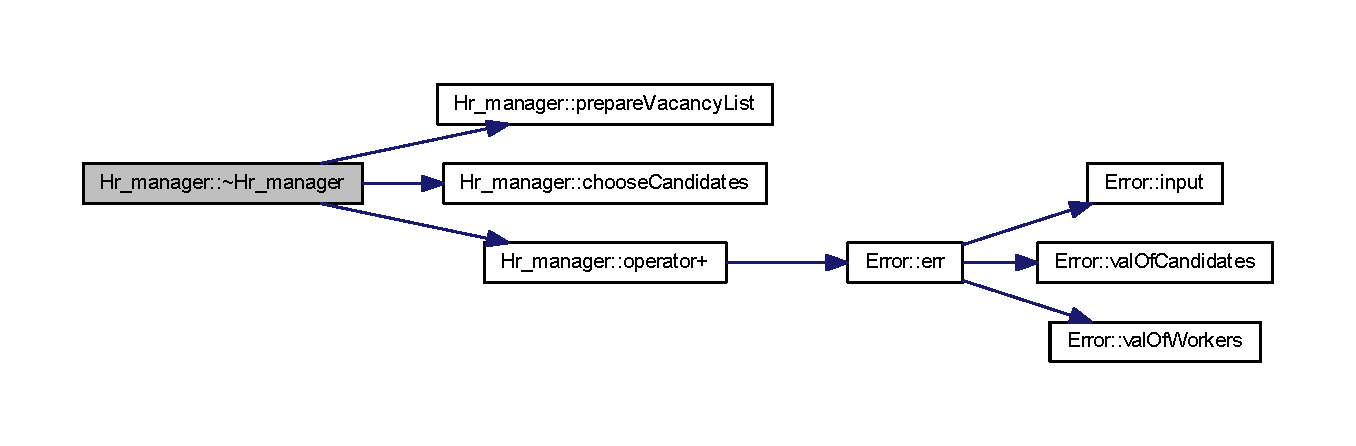
\includegraphics[width=350pt]{class_hr__manager_a6713d753a80cf4346da53d52876e751f_cgraph}
\end{center}
\end{figure}


\subsection{Member Function Documentation}
\hypertarget{class_hr__manager_ad172002747343f207758c2ea76d6e480}{}\label{class_hr__manager_ad172002747343f207758c2ea76d6e480} 
\index{Hr\+\_\+manager@{Hr\+\_\+manager}!choose\+Candidates@{choose\+Candidates}}
\index{choose\+Candidates@{choose\+Candidates}!Hr\+\_\+manager@{Hr\+\_\+manager}}
\subsubsection{\texorpdfstring{choose\+Candidates()}{chooseCandidates()}}
{\footnotesize\ttfamily void Hr\+\_\+manager\+::choose\+Candidates (\begin{DoxyParamCaption}\item[{std\+::vector$<$ std\+::string $>$}]{list }\end{DoxyParamCaption})}

Here is the caller graph for this function\+:
\nopagebreak
\begin{figure}[H]
\begin{center}
\leavevmode
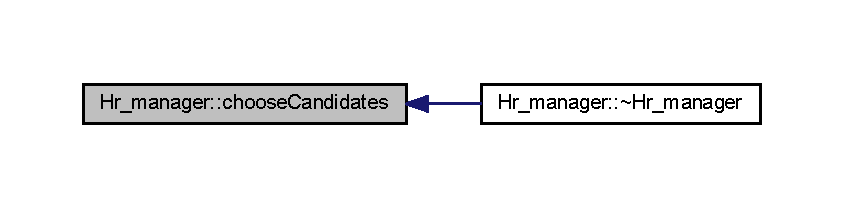
\includegraphics[width=350pt]{class_hr__manager_ad172002747343f207758c2ea76d6e480_icgraph}
\end{center}
\end{figure}
\hypertarget{class_hr__manager_a3315b88815233ab95cd924280086d8a9}{}\label{class_hr__manager_a3315b88815233ab95cd924280086d8a9} 
\index{Hr\+\_\+manager@{Hr\+\_\+manager}!operator+@{operator+}}
\index{operator+@{operator+}!Hr\+\_\+manager@{Hr\+\_\+manager}}
\subsubsection{\texorpdfstring{operator+()}{operator+()}}
{\footnotesize\ttfamily \hyperlink{class_hr__manager}{Hr\+\_\+manager} Hr\+\_\+manager\+::operator+ (\begin{DoxyParamCaption}\item[{\hyperlink{class_candidate}{Candidate} \&}]{right }\end{DoxyParamCaption})}

Here is the call graph for this function\+:
\nopagebreak
\begin{figure}[H]
\begin{center}
\leavevmode
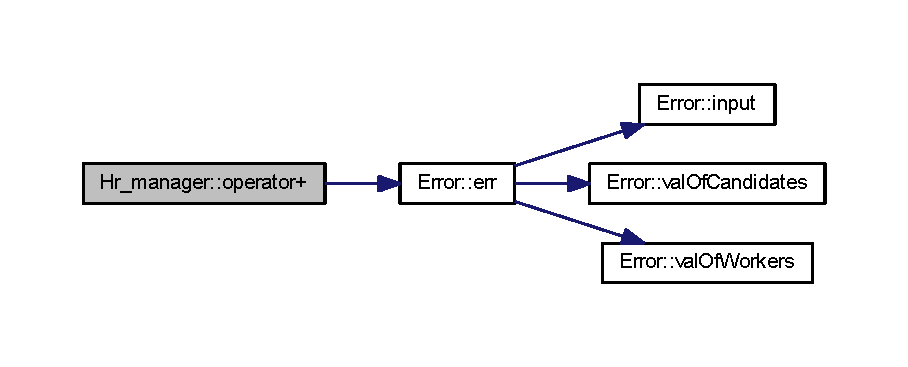
\includegraphics[width=350pt]{class_hr__manager_a3315b88815233ab95cd924280086d8a9_cgraph}
\end{center}
\end{figure}
Here is the caller graph for this function\+:
\nopagebreak
\begin{figure}[H]
\begin{center}
\leavevmode
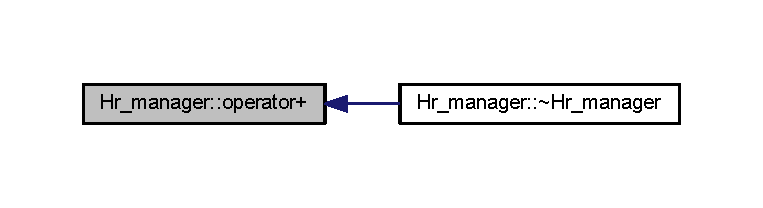
\includegraphics[width=350pt]{class_hr__manager_a3315b88815233ab95cd924280086d8a9_icgraph}
\end{center}
\end{figure}
\hypertarget{class_hr__manager_a579ebdb8579aace02b9c2d2f29051c77}{}\label{class_hr__manager_a579ebdb8579aace02b9c2d2f29051c77} 
\index{Hr\+\_\+manager@{Hr\+\_\+manager}!prepare\+Vacancy\+List@{prepare\+Vacancy\+List}}
\index{prepare\+Vacancy\+List@{prepare\+Vacancy\+List}!Hr\+\_\+manager@{Hr\+\_\+manager}}
\subsubsection{\texorpdfstring{prepare\+Vacancy\+List()}{prepareVacancyList()}}
{\footnotesize\ttfamily std\+::vector$<$ std\+::string $>$ Hr\+\_\+manager\+::prepare\+Vacancy\+List (\begin{DoxyParamCaption}\item[{int}]{max,  }\item[{int}]{cur }\end{DoxyParamCaption})}

Here is the caller graph for this function\+:
\nopagebreak
\begin{figure}[H]
\begin{center}
\leavevmode
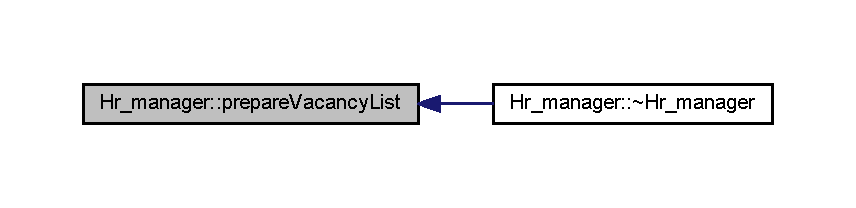
\includegraphics[width=350pt]{class_hr__manager_a579ebdb8579aace02b9c2d2f29051c77_icgraph}
\end{center}
\end{figure}
\hypertarget{class_hr__manager_a760e884af11ec93a1dbf3769cdf34adf}{}\label{class_hr__manager_a760e884af11ec93a1dbf3769cdf34adf} 
\index{Hr\+\_\+manager@{Hr\+\_\+manager}!show\+Position@{show\+Position}}
\index{show\+Position@{show\+Position}!Hr\+\_\+manager@{Hr\+\_\+manager}}
\subsubsection{\texorpdfstring{show\+Position()}{showPosition()}}
{\footnotesize\ttfamily void Hr\+\_\+manager\+::show\+Position (\begin{DoxyParamCaption}{ }\end{DoxyParamCaption})\hspace{0.3cm}{\ttfamily [inline]}, {\ttfamily [virtual]}}



Reimplemented from \hyperlink{class_worker_aaba3653d2ee34cb8834e8d631989090f}{Worker}.



\subsection{Friends And Related Function Documentation}
\hypertarget{class_hr__manager_a954d2b0eb5d6bd979593a3d4018f52c5}{}\label{class_hr__manager_a954d2b0eb5d6bd979593a3d4018f52c5} 
\index{Hr\+\_\+manager@{Hr\+\_\+manager}!operator$<$$<$@{operator$<$$<$}}
\index{operator$<$$<$@{operator$<$$<$}!Hr\+\_\+manager@{Hr\+\_\+manager}}
\subsubsection{\texorpdfstring{operator$<$$<$}{operator<<}}
{\footnotesize\ttfamily std\+::ostream\& operator$<$$<$ (\begin{DoxyParamCaption}\item[{std\+::ostream \&}]{stream,  }\item[{\hyperlink{class_hr__manager}{Hr\+\_\+manager}}]{hrmanager }\end{DoxyParamCaption})\hspace{0.3cm}{\ttfamily [friend]}}



\subsection{Member Data Documentation}
\hypertarget{class_hr__manager_a4f136a7a1ad3c57b8463b3e627a5c5f5}{}\label{class_hr__manager_a4f136a7a1ad3c57b8463b3e627a5c5f5} 
\index{Hr\+\_\+manager@{Hr\+\_\+manager}!candidate@{candidate}}
\index{candidate@{candidate}!Hr\+\_\+manager@{Hr\+\_\+manager}}
\subsubsection{\texorpdfstring{candidate}{candidate}}
{\footnotesize\ttfamily std\+::vector$<$\hyperlink{class_candidate}{Candidate}$\ast$$>$ Hr\+\_\+manager\+::candidate}



The documentation for this class was generated from the following files\+:\begin{DoxyCompactItemize}
\item 
\hyperlink{_hr__manager_8h}{Hr\+\_\+manager.\+h}\item 
\hyperlink{_hr__manager_8cpp}{Hr\+\_\+manager.\+cpp}\end{DoxyCompactItemize}

\hypertarget{class_interview}{}\section{Interview Class Reference}
\label{class_interview}\index{Interview@{Interview}}


{\ttfamily \#include $<$Interview.\+h$>$}



Collaboration diagram for Interview\+:
\nopagebreak
\begin{figure}[H]
\begin{center}
\leavevmode
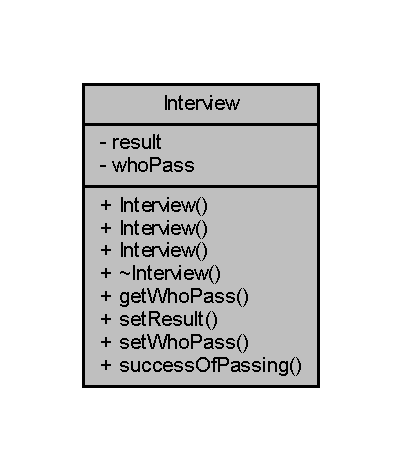
\includegraphics[width=193pt]{class_interview__coll__graph}
\end{center}
\end{figure}
\subsection*{Public Member Functions}
\begin{DoxyCompactItemize}
\item 
\hyperlink{class_interview_a18c238c7fd5e7a118b0cd41f35f93360}{Interview} ()
\item 
\hyperlink{class_interview_aedb4e2b612dd1c811957eeba48e7cff2}{Interview} (bool \hyperlink{class_interview_aa456226f23acfdb23a6c94eab33e3cbb}{result})
\item 
\hyperlink{class_interview_a5910c3f8fd63842d118ffde49bce514b}{Interview} (\hyperlink{class_interview}{Interview} \&s\+Interview)
\item 
\hyperlink{class_interview_a5d38984d9695b62a2e4aabcf5295810c}{$\sim$\+Interview} ()
\item 
std\+::string \hyperlink{class_interview_adef4bd6cdccfc2a3e610ee2ef2489dcd}{get\+Who\+Pass} (void)
\item 
void \hyperlink{class_interview_abbd0885e4e3823bb65951cc0bb647d6b}{set\+Result} (bool r)
\item 
void \hyperlink{class_interview_ae7b385238b18a719812f41ea96040c3e}{set\+Who\+Pass} (std\+::string name)
\item 
bool \hyperlink{class_interview_a20d7ee5c6fd7c030857b21c39b1d1e1b}{success\+Of\+Passing} (void)
\end{DoxyCompactItemize}
\subsection*{Private Attributes}
\begin{DoxyCompactItemize}
\item 
bool \hyperlink{class_interview_aa456226f23acfdb23a6c94eab33e3cbb}{result}
\item 
std\+::string \hyperlink{class_interview_a8621e9f225dce314abaf77b7854649f6}{who\+Pass}
\end{DoxyCompactItemize}
\subsection*{Friends}
\begin{DoxyCompactItemize}
\item 
std\+::ostream \& \hyperlink{class_interview_aa32d4e45baf6b6c73433889c6988079f}{operator$<$$<$} (std\+::ostream \&stream, \hyperlink{class_interview}{Interview} interview)
\end{DoxyCompactItemize}


\subsection{Constructor \& Destructor Documentation}
\hypertarget{class_interview_a18c238c7fd5e7a118b0cd41f35f93360}{}\label{class_interview_a18c238c7fd5e7a118b0cd41f35f93360} 
\index{Interview@{Interview}!Interview@{Interview}}
\index{Interview@{Interview}!Interview@{Interview}}
\subsubsection{\texorpdfstring{Interview()}{Interview()}\hspace{0.1cm}{\footnotesize\ttfamily [1/3]}}
{\footnotesize\ttfamily Interview\+::\+Interview (\begin{DoxyParamCaption}{ }\end{DoxyParamCaption})\hspace{0.3cm}{\ttfamily [inline]}}

\hypertarget{class_interview_aedb4e2b612dd1c811957eeba48e7cff2}{}\label{class_interview_aedb4e2b612dd1c811957eeba48e7cff2} 
\index{Interview@{Interview}!Interview@{Interview}}
\index{Interview@{Interview}!Interview@{Interview}}
\subsubsection{\texorpdfstring{Interview()}{Interview()}\hspace{0.1cm}{\footnotesize\ttfamily [2/3]}}
{\footnotesize\ttfamily Interview\+::\+Interview (\begin{DoxyParamCaption}\item[{bool}]{result }\end{DoxyParamCaption})\hspace{0.3cm}{\ttfamily [inline]}}

\hypertarget{class_interview_a5910c3f8fd63842d118ffde49bce514b}{}\label{class_interview_a5910c3f8fd63842d118ffde49bce514b} 
\index{Interview@{Interview}!Interview@{Interview}}
\index{Interview@{Interview}!Interview@{Interview}}
\subsubsection{\texorpdfstring{Interview()}{Interview()}\hspace{0.1cm}{\footnotesize\ttfamily [3/3]}}
{\footnotesize\ttfamily Interview\+::\+Interview (\begin{DoxyParamCaption}\item[{\hyperlink{class_interview}{Interview} \&}]{s\+Interview }\end{DoxyParamCaption})\hspace{0.3cm}{\ttfamily [inline]}}

\hypertarget{class_interview_a5d38984d9695b62a2e4aabcf5295810c}{}\label{class_interview_a5d38984d9695b62a2e4aabcf5295810c} 
\index{Interview@{Interview}!````~Interview@{$\sim$\+Interview}}
\index{````~Interview@{$\sim$\+Interview}!Interview@{Interview}}
\subsubsection{\texorpdfstring{$\sim$\+Interview()}{~Interview()}}
{\footnotesize\ttfamily Interview\+::$\sim$\+Interview (\begin{DoxyParamCaption}{ }\end{DoxyParamCaption})\hspace{0.3cm}{\ttfamily [inline]}}



\subsection{Member Function Documentation}
\hypertarget{class_interview_adef4bd6cdccfc2a3e610ee2ef2489dcd}{}\label{class_interview_adef4bd6cdccfc2a3e610ee2ef2489dcd} 
\index{Interview@{Interview}!get\+Who\+Pass@{get\+Who\+Pass}}
\index{get\+Who\+Pass@{get\+Who\+Pass}!Interview@{Interview}}
\subsubsection{\texorpdfstring{get\+Who\+Pass()}{getWhoPass()}}
{\footnotesize\ttfamily std\+::string Interview\+::get\+Who\+Pass (\begin{DoxyParamCaption}\item[{void}]{ }\end{DoxyParamCaption})\hspace{0.3cm}{\ttfamily [inline]}}

\hypertarget{class_interview_abbd0885e4e3823bb65951cc0bb647d6b}{}\label{class_interview_abbd0885e4e3823bb65951cc0bb647d6b} 
\index{Interview@{Interview}!set\+Result@{set\+Result}}
\index{set\+Result@{set\+Result}!Interview@{Interview}}
\subsubsection{\texorpdfstring{set\+Result()}{setResult()}}
{\footnotesize\ttfamily void Interview\+::set\+Result (\begin{DoxyParamCaption}\item[{bool}]{r }\end{DoxyParamCaption})\hspace{0.3cm}{\ttfamily [inline]}}

\hypertarget{class_interview_ae7b385238b18a719812f41ea96040c3e}{}\label{class_interview_ae7b385238b18a719812f41ea96040c3e} 
\index{Interview@{Interview}!set\+Who\+Pass@{set\+Who\+Pass}}
\index{set\+Who\+Pass@{set\+Who\+Pass}!Interview@{Interview}}
\subsubsection{\texorpdfstring{set\+Who\+Pass()}{setWhoPass()}}
{\footnotesize\ttfamily void Interview\+::set\+Who\+Pass (\begin{DoxyParamCaption}\item[{std\+::string}]{name }\end{DoxyParamCaption})\hspace{0.3cm}{\ttfamily [inline]}}

\hypertarget{class_interview_a20d7ee5c6fd7c030857b21c39b1d1e1b}{}\label{class_interview_a20d7ee5c6fd7c030857b21c39b1d1e1b} 
\index{Interview@{Interview}!success\+Of\+Passing@{success\+Of\+Passing}}
\index{success\+Of\+Passing@{success\+Of\+Passing}!Interview@{Interview}}
\subsubsection{\texorpdfstring{success\+Of\+Passing()}{successOfPassing()}}
{\footnotesize\ttfamily bool Interview\+::success\+Of\+Passing (\begin{DoxyParamCaption}\item[{void}]{ }\end{DoxyParamCaption})\hspace{0.3cm}{\ttfamily [inline]}}



\subsection{Friends And Related Function Documentation}
\hypertarget{class_interview_aa32d4e45baf6b6c73433889c6988079f}{}\label{class_interview_aa32d4e45baf6b6c73433889c6988079f} 
\index{Interview@{Interview}!operator$<$$<$@{operator$<$$<$}}
\index{operator$<$$<$@{operator$<$$<$}!Interview@{Interview}}
\subsubsection{\texorpdfstring{operator$<$$<$}{operator<<}}
{\footnotesize\ttfamily std\+::ostream\& operator$<$$<$ (\begin{DoxyParamCaption}\item[{std\+::ostream \&}]{stream,  }\item[{\hyperlink{class_interview}{Interview}}]{interview }\end{DoxyParamCaption})\hspace{0.3cm}{\ttfamily [friend]}}



\subsection{Member Data Documentation}
\hypertarget{class_interview_aa456226f23acfdb23a6c94eab33e3cbb}{}\label{class_interview_aa456226f23acfdb23a6c94eab33e3cbb} 
\index{Interview@{Interview}!result@{result}}
\index{result@{result}!Interview@{Interview}}
\subsubsection{\texorpdfstring{result}{result}}
{\footnotesize\ttfamily bool Interview\+::result\hspace{0.3cm}{\ttfamily [private]}}

\hypertarget{class_interview_a8621e9f225dce314abaf77b7854649f6}{}\label{class_interview_a8621e9f225dce314abaf77b7854649f6} 
\index{Interview@{Interview}!who\+Pass@{who\+Pass}}
\index{who\+Pass@{who\+Pass}!Interview@{Interview}}
\subsubsection{\texorpdfstring{who\+Pass}{whoPass}}
{\footnotesize\ttfamily std\+::string Interview\+::who\+Pass\hspace{0.3cm}{\ttfamily [private]}}



The documentation for this class was generated from the following file\+:\begin{DoxyCompactItemize}
\item 
\hyperlink{_interview_8h}{Interview.\+h}\end{DoxyCompactItemize}

\hypertarget{class_it__company}{}\section{It\+\_\+company Class Reference}
\label{class_it__company}\index{It\+\_\+company@{It\+\_\+company}}


{\ttfamily \#include $<$It\+\_\+company.\+h$>$}



Collaboration diagram for It\+\_\+company\+:
\nopagebreak
\begin{figure}[H]
\begin{center}
\leavevmode
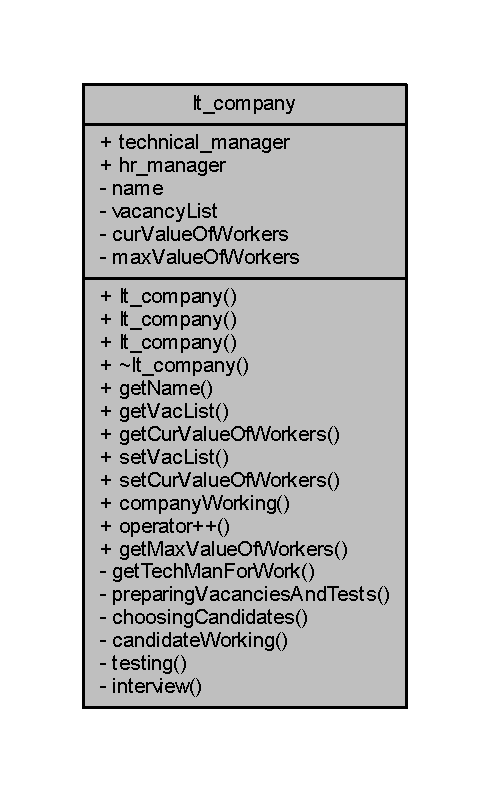
\includegraphics[width=235pt]{class_it__company__coll__graph}
\end{center}
\end{figure}
\subsection*{Public Member Functions}
\begin{DoxyCompactItemize}
\item 
\hyperlink{class_it__company_a586ce8103147bcb474965fbe92b029ae}{It\+\_\+company} ()
\item 
\hyperlink{class_it__company_aef3374e7fe0caae3e395e18418200112}{It\+\_\+company} (std\+::string \hyperlink{class_it__company_a99894304639dab6b416f697dc7e81d52}{name}, std\+::vector$<$ std\+::string $>$ \hyperlink{main_8cpp_a5ea078e5bfa9aefe80362a0a1a33edce}{vacancies}, int \hyperlink{class_it__company_ac48dbef2db2cad83837c89efdc69b9c9}{cur\+Value\+Of\+Workers})
\item 
\hyperlink{class_it__company_adbd662e9e7bc67642283301274a9326b}{It\+\_\+company} (\hyperlink{class_it__company}{It\+\_\+company} \&s\+It\+\_\+company)
\item 
\hyperlink{class_it__company_abea4fe4b9e6229c4b7e84881cf124975}{$\sim$\+It\+\_\+company} ()
\item 
std\+::string \hyperlink{class_it__company_a83fff670c4a7271486f9632db1bf4d77}{get\+Name} (void) const
\item 
std\+::vector$<$ std\+::string $>$ \hyperlink{class_it__company_a292596bb863a09f2983cb955979a8bb9}{get\+Vac\+List} (void) const
\item 
int \hyperlink{class_it__company_aadb84a911a10ad83f6e9a84558a1d4df}{get\+Cur\+Value\+Of\+Workers} (void) const
\item 
void \hyperlink{class_it__company_a079be9a566c94860e31acdb0c2953536}{set\+Vac\+List} (std\+::vector$<$ std\+::string $>$ vl)
\item 
void \hyperlink{class_it__company_ae06d651e9611d19f02bc1c7f29f2e988}{set\+Cur\+Value\+Of\+Workers} (int cur)
\item 
void \hyperlink{class_it__company_a57d8e8056fb6753cef0a6acd80a801dd}{company\+Working} ()
\item 
\hyperlink{class_it__company}{It\+\_\+company} \& \hyperlink{class_it__company_ae83add85a00be1e24cdce48aa72678de}{operator++} ()
\end{DoxyCompactItemize}
\subsection*{Static Public Member Functions}
\begin{DoxyCompactItemize}
\item 
static const int \hyperlink{class_it__company_a11e4104cfd2c51f89f9d10b290c8eaaa}{get\+Max\+Value\+Of\+Workers} (void)
\end{DoxyCompactItemize}
\subsection*{Public Attributes}
\begin{DoxyCompactItemize}
\item 
std\+::vector$<$ \hyperlink{class_technical__manager}{Technical\+\_\+manager} $>$ \hyperlink{class_it__company_af2285094fb07bcf0a9f3a4c1d8a407d3}{technical\+\_\+manager}
\item 
std\+::vector$<$ \hyperlink{class_hr__manager}{Hr\+\_\+manager} $>$ \hyperlink{class_it__company_ae0e3f81754b1433c6dfb5ebe96f620d1}{hr\+\_\+manager}
\end{DoxyCompactItemize}
\subsection*{Private Member Functions}
\begin{DoxyCompactItemize}
\item 
\hyperlink{class_technical__manager}{Technical\+\_\+manager} $\ast$ \hyperlink{class_it__company_aa0b755bdb8d21b72bc42403b90b62898}{get\+Tech\+Man\+For\+Work} (void)
\item 
void \hyperlink{class_it__company_ab5f464351646bc6458640391f5eab298}{preparing\+Vacancies\+And\+Tests} ()
\item 
void \hyperlink{class_it__company_aead10e44d7215787e8e532e2e0463d0d}{choosing\+Candidates} ()
\item 
void \hyperlink{class_it__company_aaca00d2170e5b58ec725a35afb0f4b59}{candidate\+Working} (int time, std\+::vector$<$ std\+::vector$<$ std\+::string $>$$>$ \&all\+Answers, std\+::multimap$<$ int, int $>$ \&cand\+Index)
\item 
void \hyperlink{class_it__company_a2c7a94d7f82fb700c0d1f369423ad45f}{testing} (std\+::vector$<$ std\+::vector$<$ std\+::string $>$$>$ \&all\+Answers, std\+::multimap$<$ int, int $>$ \&cand\+Index)
\item 
void \hyperlink{class_it__company_a0d05d1b25d00b221bbb66e57332dea08}{interview} ()
\end{DoxyCompactItemize}
\subsection*{Private Attributes}
\begin{DoxyCompactItemize}
\item 
const std\+::string \hyperlink{class_it__company_a99894304639dab6b416f697dc7e81d52}{name}
\item 
std\+::vector$<$ std\+::string $>$ \hyperlink{class_it__company_a06d700346a5bcd94c1f265f3bb65143f}{vacancy\+List}
\item 
int \hyperlink{class_it__company_ac48dbef2db2cad83837c89efdc69b9c9}{cur\+Value\+Of\+Workers}
\end{DoxyCompactItemize}
\subsection*{Static Private Attributes}
\begin{DoxyCompactItemize}
\item 
static const int \hyperlink{class_it__company_ac71fd3642622747e9e543b5a193ba525}{max\+Value\+Of\+Workers} = 3
\end{DoxyCompactItemize}
\subsection*{Friends}
\begin{DoxyCompactItemize}
\item 
std\+::ostream \& \hyperlink{class_it__company_a962e1dda6d2c3075501e63a8d62693f7}{operator$<$$<$} (std\+::ostream \&stream, \hyperlink{class_it__company}{It\+\_\+company} itcompany)
\end{DoxyCompactItemize}


\subsection{Constructor \& Destructor Documentation}
\hypertarget{class_it__company_a586ce8103147bcb474965fbe92b029ae}{}\label{class_it__company_a586ce8103147bcb474965fbe92b029ae} 
\index{It\+\_\+company@{It\+\_\+company}!It\+\_\+company@{It\+\_\+company}}
\index{It\+\_\+company@{It\+\_\+company}!It\+\_\+company@{It\+\_\+company}}
\subsubsection{\texorpdfstring{It\+\_\+company()}{It\_company()}\hspace{0.1cm}{\footnotesize\ttfamily [1/3]}}
{\footnotesize\ttfamily It\+\_\+company\+::\+It\+\_\+company (\begin{DoxyParamCaption}{ }\end{DoxyParamCaption})\hspace{0.3cm}{\ttfamily [inline]}}

\hypertarget{class_it__company_aef3374e7fe0caae3e395e18418200112}{}\label{class_it__company_aef3374e7fe0caae3e395e18418200112} 
\index{It\+\_\+company@{It\+\_\+company}!It\+\_\+company@{It\+\_\+company}}
\index{It\+\_\+company@{It\+\_\+company}!It\+\_\+company@{It\+\_\+company}}
\subsubsection{\texorpdfstring{It\+\_\+company()}{It\_company()}\hspace{0.1cm}{\footnotesize\ttfamily [2/3]}}
{\footnotesize\ttfamily It\+\_\+company\+::\+It\+\_\+company (\begin{DoxyParamCaption}\item[{std\+::string}]{name,  }\item[{std\+::vector$<$ std\+::string $>$}]{vacancies,  }\item[{int}]{cur\+Value\+Of\+Workers }\end{DoxyParamCaption})\hspace{0.3cm}{\ttfamily [inline]}}

\hypertarget{class_it__company_adbd662e9e7bc67642283301274a9326b}{}\label{class_it__company_adbd662e9e7bc67642283301274a9326b} 
\index{It\+\_\+company@{It\+\_\+company}!It\+\_\+company@{It\+\_\+company}}
\index{It\+\_\+company@{It\+\_\+company}!It\+\_\+company@{It\+\_\+company}}
\subsubsection{\texorpdfstring{It\+\_\+company()}{It\_company()}\hspace{0.1cm}{\footnotesize\ttfamily [3/3]}}
{\footnotesize\ttfamily It\+\_\+company\+::\+It\+\_\+company (\begin{DoxyParamCaption}\item[{\hyperlink{class_it__company}{It\+\_\+company} \&}]{s\+It\+\_\+company }\end{DoxyParamCaption})\hspace{0.3cm}{\ttfamily [inline]}}

\hypertarget{class_it__company_abea4fe4b9e6229c4b7e84881cf124975}{}\label{class_it__company_abea4fe4b9e6229c4b7e84881cf124975} 
\index{It\+\_\+company@{It\+\_\+company}!````~It\+\_\+company@{$\sim$\+It\+\_\+company}}
\index{````~It\+\_\+company@{$\sim$\+It\+\_\+company}!It\+\_\+company@{It\+\_\+company}}
\subsubsection{\texorpdfstring{$\sim$\+It\+\_\+company()}{~It\_company()}}
{\footnotesize\ttfamily It\+\_\+company\+::$\sim$\+It\+\_\+company (\begin{DoxyParamCaption}{ }\end{DoxyParamCaption})\hspace{0.3cm}{\ttfamily [inline]}}



\subsection{Member Function Documentation}
\hypertarget{class_it__company_aaca00d2170e5b58ec725a35afb0f4b59}{}\label{class_it__company_aaca00d2170e5b58ec725a35afb0f4b59} 
\index{It\+\_\+company@{It\+\_\+company}!candidate\+Working@{candidate\+Working}}
\index{candidate\+Working@{candidate\+Working}!It\+\_\+company@{It\+\_\+company}}
\subsubsection{\texorpdfstring{candidate\+Working()}{candidateWorking()}}
{\footnotesize\ttfamily void It\+\_\+company\+::candidate\+Working (\begin{DoxyParamCaption}\item[{int}]{time,  }\item[{std\+::vector$<$ std\+::vector$<$ std\+::string $>$$>$ \&}]{all\+Answers,  }\item[{std\+::multimap$<$ int, int $>$ \&}]{cand\+Index }\end{DoxyParamCaption})\hspace{0.3cm}{\ttfamily [private]}}

Here is the call graph for this function\+:
\nopagebreak
\begin{figure}[H]
\begin{center}
\leavevmode
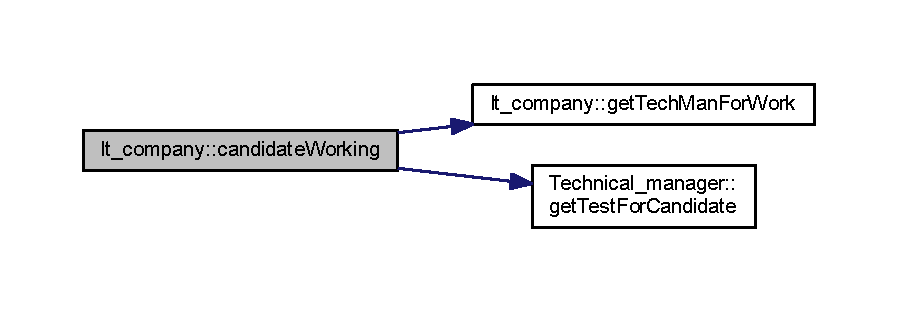
\includegraphics[width=350pt]{class_it__company_aaca00d2170e5b58ec725a35afb0f4b59_cgraph}
\end{center}
\end{figure}
Here is the caller graph for this function\+:
\nopagebreak
\begin{figure}[H]
\begin{center}
\leavevmode
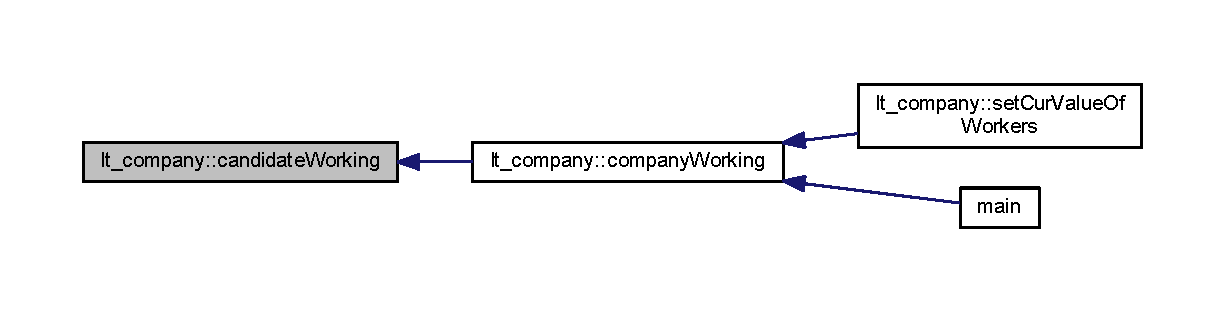
\includegraphics[width=350pt]{class_it__company_aaca00d2170e5b58ec725a35afb0f4b59_icgraph}
\end{center}
\end{figure}
\hypertarget{class_it__company_aead10e44d7215787e8e532e2e0463d0d}{}\label{class_it__company_aead10e44d7215787e8e532e2e0463d0d} 
\index{It\+\_\+company@{It\+\_\+company}!choosing\+Candidates@{choosing\+Candidates}}
\index{choosing\+Candidates@{choosing\+Candidates}!It\+\_\+company@{It\+\_\+company}}
\subsubsection{\texorpdfstring{choosing\+Candidates()}{choosingCandidates()}}
{\footnotesize\ttfamily void It\+\_\+company\+::choosing\+Candidates (\begin{DoxyParamCaption}{ }\end{DoxyParamCaption})\hspace{0.3cm}{\ttfamily [private]}}

Here is the caller graph for this function\+:
\nopagebreak
\begin{figure}[H]
\begin{center}
\leavevmode
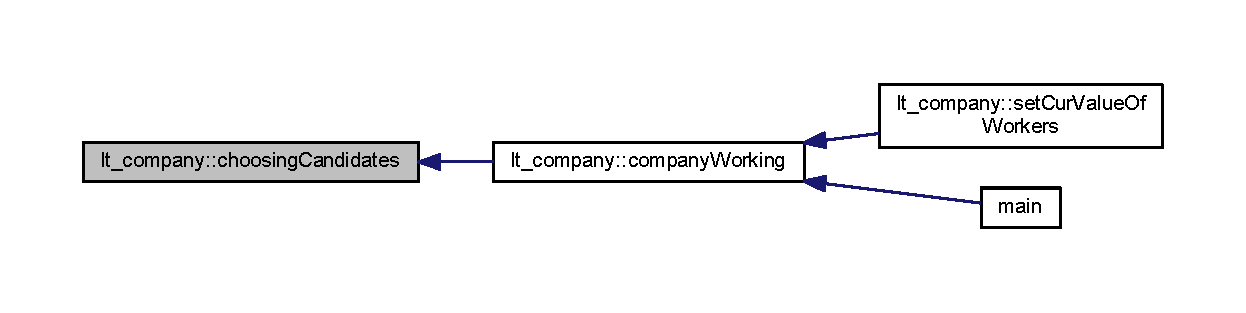
\includegraphics[width=350pt]{class_it__company_aead10e44d7215787e8e532e2e0463d0d_icgraph}
\end{center}
\end{figure}
\hypertarget{class_it__company_a57d8e8056fb6753cef0a6acd80a801dd}{}\label{class_it__company_a57d8e8056fb6753cef0a6acd80a801dd} 
\index{It\+\_\+company@{It\+\_\+company}!company\+Working@{company\+Working}}
\index{company\+Working@{company\+Working}!It\+\_\+company@{It\+\_\+company}}
\subsubsection{\texorpdfstring{company\+Working()}{companyWorking()}}
{\footnotesize\ttfamily void It\+\_\+company\+::company\+Working (\begin{DoxyParamCaption}{ }\end{DoxyParamCaption})}

Here is the call graph for this function\+:
\nopagebreak
\begin{figure}[H]
\begin{center}
\leavevmode
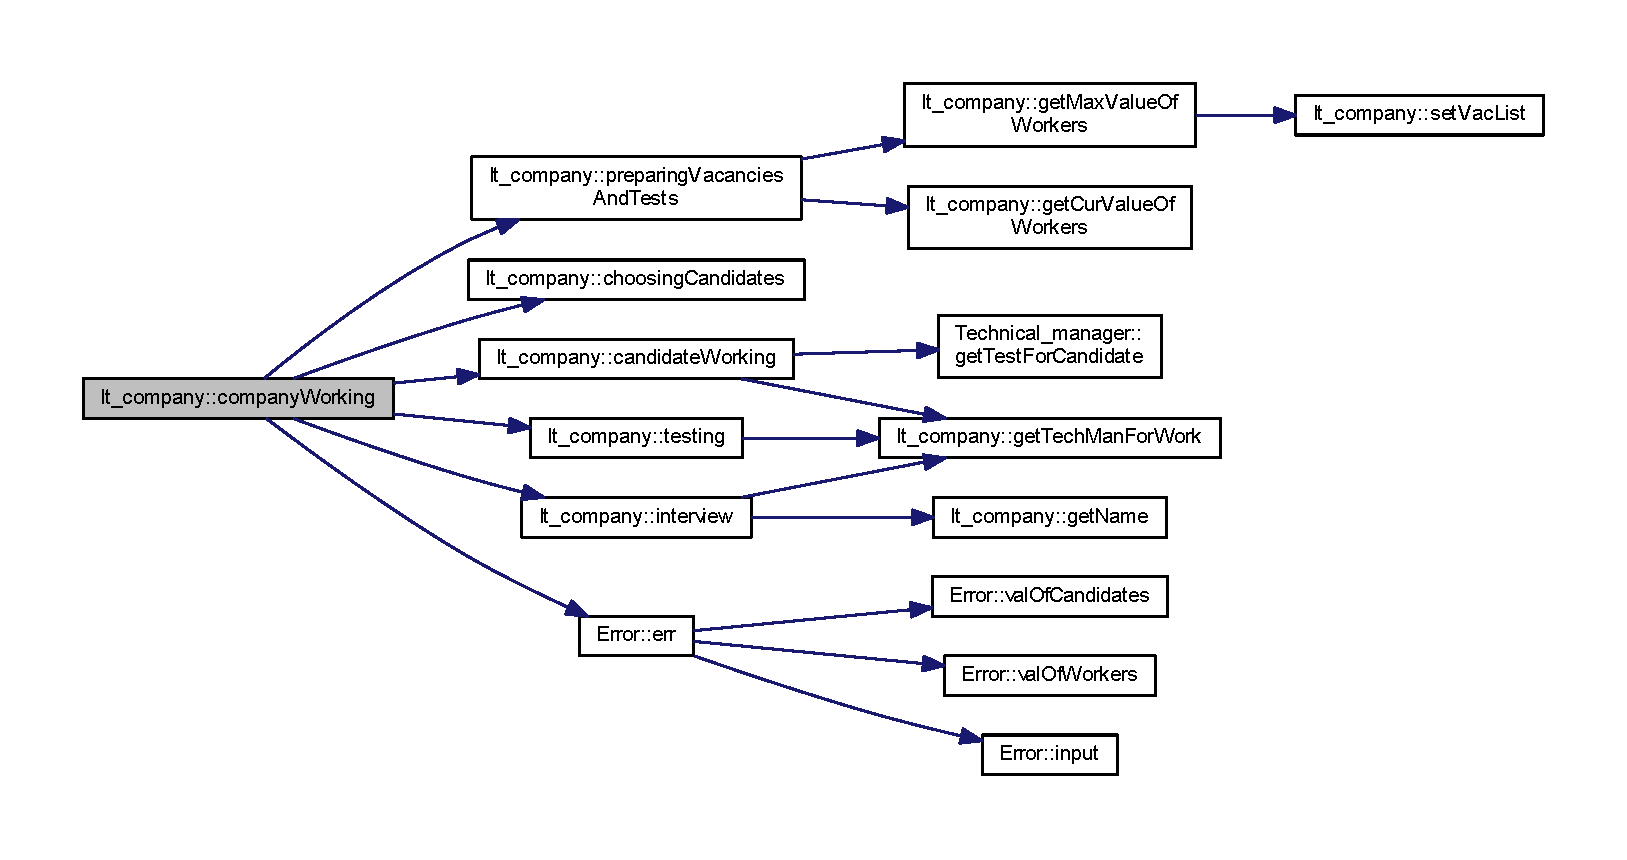
\includegraphics[width=350pt]{class_it__company_a57d8e8056fb6753cef0a6acd80a801dd_cgraph}
\end{center}
\end{figure}
Here is the caller graph for this function\+:
\nopagebreak
\begin{figure}[H]
\begin{center}
\leavevmode
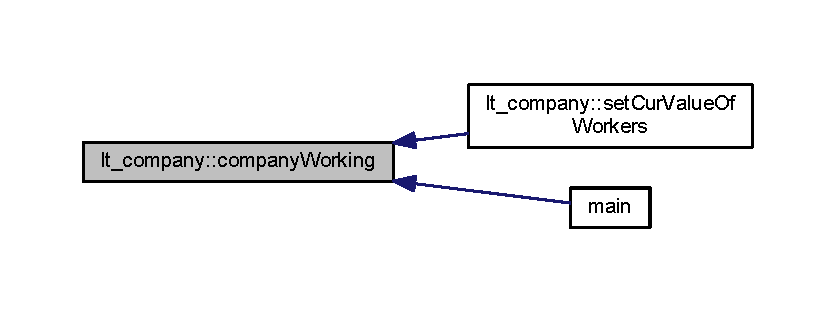
\includegraphics[width=350pt]{class_it__company_a57d8e8056fb6753cef0a6acd80a801dd_icgraph}
\end{center}
\end{figure}
\hypertarget{class_it__company_aadb84a911a10ad83f6e9a84558a1d4df}{}\label{class_it__company_aadb84a911a10ad83f6e9a84558a1d4df} 
\index{It\+\_\+company@{It\+\_\+company}!get\+Cur\+Value\+Of\+Workers@{get\+Cur\+Value\+Of\+Workers}}
\index{get\+Cur\+Value\+Of\+Workers@{get\+Cur\+Value\+Of\+Workers}!It\+\_\+company@{It\+\_\+company}}
\subsubsection{\texorpdfstring{get\+Cur\+Value\+Of\+Workers()}{getCurValueOfWorkers()}}
{\footnotesize\ttfamily int It\+\_\+company\+::get\+Cur\+Value\+Of\+Workers (\begin{DoxyParamCaption}\item[{void}]{ }\end{DoxyParamCaption}) const\hspace{0.3cm}{\ttfamily [inline]}}

Here is the caller graph for this function\+:
\nopagebreak
\begin{figure}[H]
\begin{center}
\leavevmode
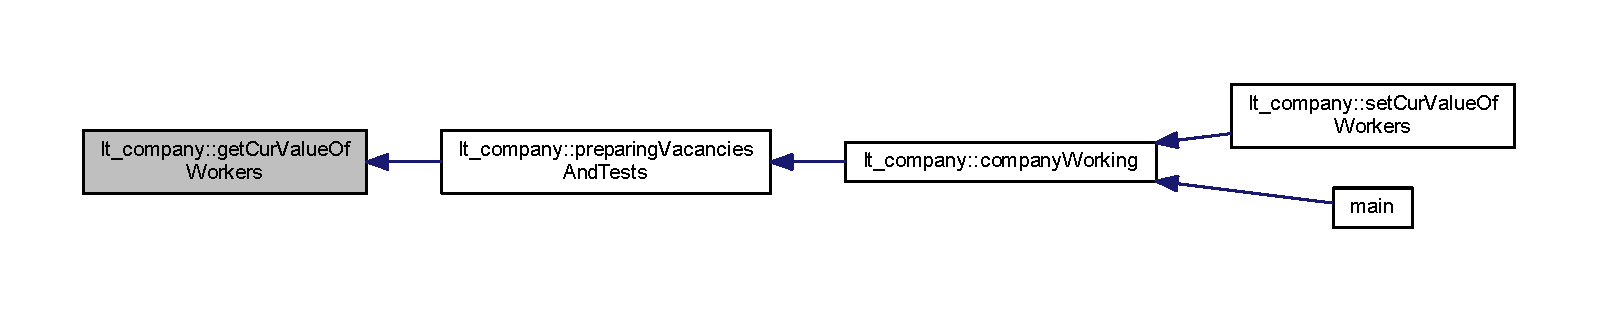
\includegraphics[width=350pt]{class_it__company_aadb84a911a10ad83f6e9a84558a1d4df_icgraph}
\end{center}
\end{figure}
\hypertarget{class_it__company_a11e4104cfd2c51f89f9d10b290c8eaaa}{}\label{class_it__company_a11e4104cfd2c51f89f9d10b290c8eaaa} 
\index{It\+\_\+company@{It\+\_\+company}!get\+Max\+Value\+Of\+Workers@{get\+Max\+Value\+Of\+Workers}}
\index{get\+Max\+Value\+Of\+Workers@{get\+Max\+Value\+Of\+Workers}!It\+\_\+company@{It\+\_\+company}}
\subsubsection{\texorpdfstring{get\+Max\+Value\+Of\+Workers()}{getMaxValueOfWorkers()}}
{\footnotesize\ttfamily static const int It\+\_\+company\+::get\+Max\+Value\+Of\+Workers (\begin{DoxyParamCaption}\item[{void}]{ }\end{DoxyParamCaption})\hspace{0.3cm}{\ttfamily [inline]}, {\ttfamily [static]}}

Here is the call graph for this function\+:
\nopagebreak
\begin{figure}[H]
\begin{center}
\leavevmode
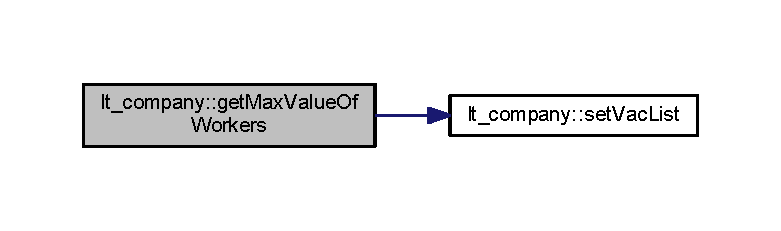
\includegraphics[width=350pt]{class_it__company_a11e4104cfd2c51f89f9d10b290c8eaaa_cgraph}
\end{center}
\end{figure}
Here is the caller graph for this function\+:
\nopagebreak
\begin{figure}[H]
\begin{center}
\leavevmode
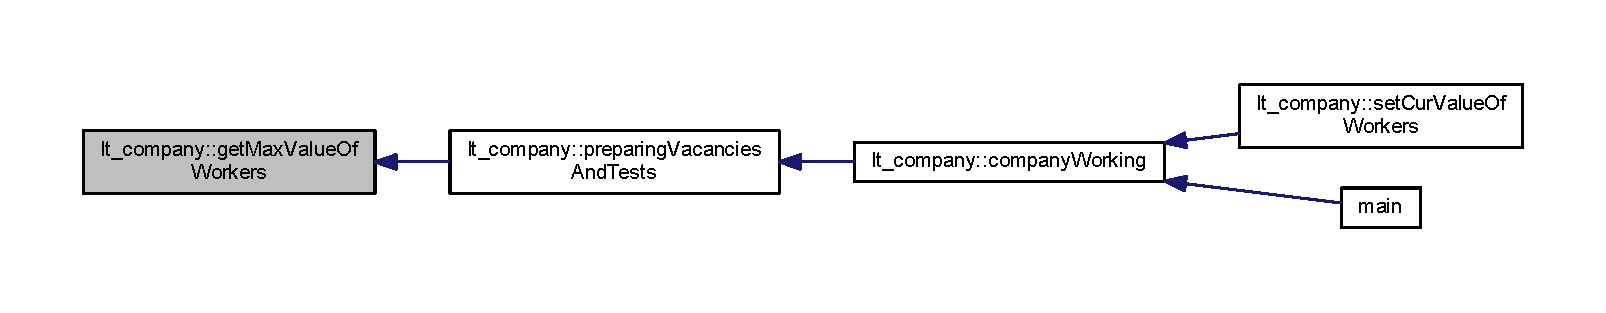
\includegraphics[width=350pt]{class_it__company_a11e4104cfd2c51f89f9d10b290c8eaaa_icgraph}
\end{center}
\end{figure}
\hypertarget{class_it__company_a83fff670c4a7271486f9632db1bf4d77}{}\label{class_it__company_a83fff670c4a7271486f9632db1bf4d77} 
\index{It\+\_\+company@{It\+\_\+company}!get\+Name@{get\+Name}}
\index{get\+Name@{get\+Name}!It\+\_\+company@{It\+\_\+company}}
\subsubsection{\texorpdfstring{get\+Name()}{getName()}}
{\footnotesize\ttfamily std\+::string It\+\_\+company\+::get\+Name (\begin{DoxyParamCaption}\item[{void}]{ }\end{DoxyParamCaption}) const\hspace{0.3cm}{\ttfamily [inline]}}

Here is the caller graph for this function\+:
\nopagebreak
\begin{figure}[H]
\begin{center}
\leavevmode
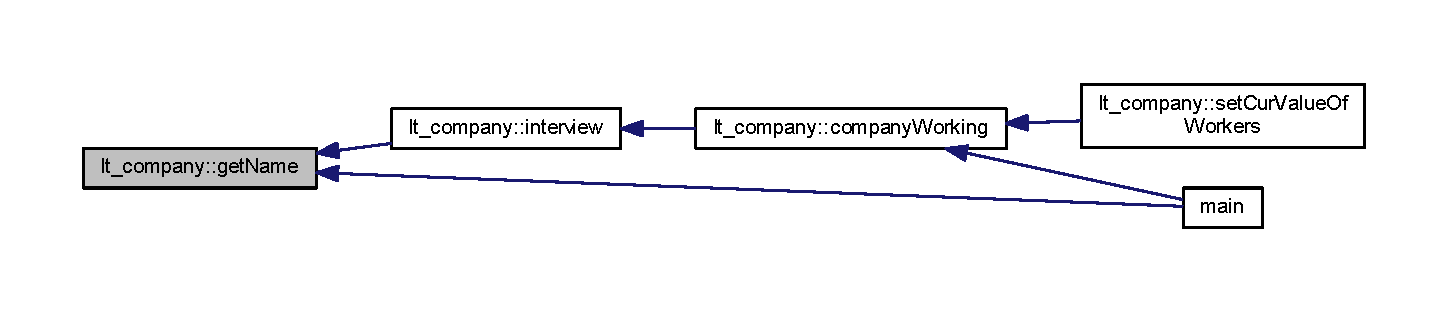
\includegraphics[width=350pt]{class_it__company_a83fff670c4a7271486f9632db1bf4d77_icgraph}
\end{center}
\end{figure}
\hypertarget{class_it__company_aa0b755bdb8d21b72bc42403b90b62898}{}\label{class_it__company_aa0b755bdb8d21b72bc42403b90b62898} 
\index{It\+\_\+company@{It\+\_\+company}!get\+Tech\+Man\+For\+Work@{get\+Tech\+Man\+For\+Work}}
\index{get\+Tech\+Man\+For\+Work@{get\+Tech\+Man\+For\+Work}!It\+\_\+company@{It\+\_\+company}}
\subsubsection{\texorpdfstring{get\+Tech\+Man\+For\+Work()}{getTechManForWork()}}
{\footnotesize\ttfamily \hyperlink{class_technical__manager}{Technical\+\_\+manager} $\ast$ It\+\_\+company\+::get\+Tech\+Man\+For\+Work (\begin{DoxyParamCaption}\item[{void}]{ }\end{DoxyParamCaption})\hspace{0.3cm}{\ttfamily [private]}}

Here is the caller graph for this function\+:
\nopagebreak
\begin{figure}[H]
\begin{center}
\leavevmode
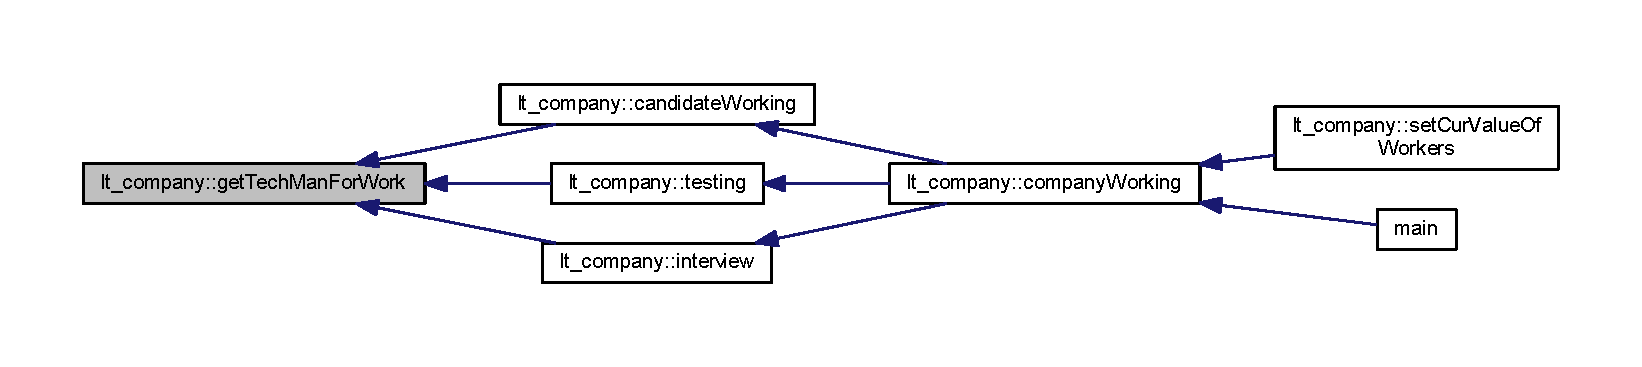
\includegraphics[width=350pt]{class_it__company_aa0b755bdb8d21b72bc42403b90b62898_icgraph}
\end{center}
\end{figure}
\hypertarget{class_it__company_a292596bb863a09f2983cb955979a8bb9}{}\label{class_it__company_a292596bb863a09f2983cb955979a8bb9} 
\index{It\+\_\+company@{It\+\_\+company}!get\+Vac\+List@{get\+Vac\+List}}
\index{get\+Vac\+List@{get\+Vac\+List}!It\+\_\+company@{It\+\_\+company}}
\subsubsection{\texorpdfstring{get\+Vac\+List()}{getVacList()}}
{\footnotesize\ttfamily std\+::vector$<$std\+::string$>$ It\+\_\+company\+::get\+Vac\+List (\begin{DoxyParamCaption}\item[{void}]{ }\end{DoxyParamCaption}) const\hspace{0.3cm}{\ttfamily [inline]}}

\hypertarget{class_it__company_a0d05d1b25d00b221bbb66e57332dea08}{}\label{class_it__company_a0d05d1b25d00b221bbb66e57332dea08} 
\index{It\+\_\+company@{It\+\_\+company}!interview@{interview}}
\index{interview@{interview}!It\+\_\+company@{It\+\_\+company}}
\subsubsection{\texorpdfstring{interview()}{interview()}}
{\footnotesize\ttfamily void It\+\_\+company\+::interview (\begin{DoxyParamCaption}{ }\end{DoxyParamCaption})\hspace{0.3cm}{\ttfamily [private]}}

Here is the call graph for this function\+:
\nopagebreak
\begin{figure}[H]
\begin{center}
\leavevmode
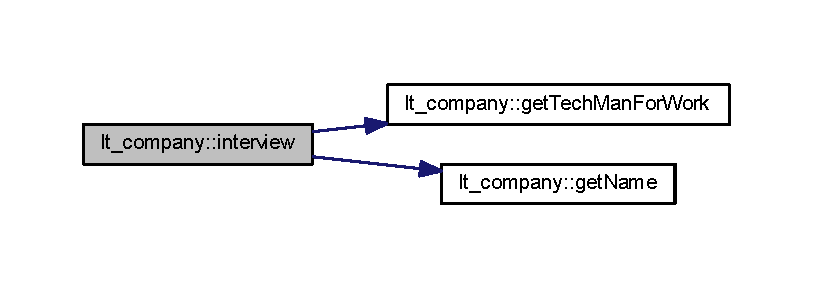
\includegraphics[width=350pt]{class_it__company_a0d05d1b25d00b221bbb66e57332dea08_cgraph}
\end{center}
\end{figure}
Here is the caller graph for this function\+:
\nopagebreak
\begin{figure}[H]
\begin{center}
\leavevmode
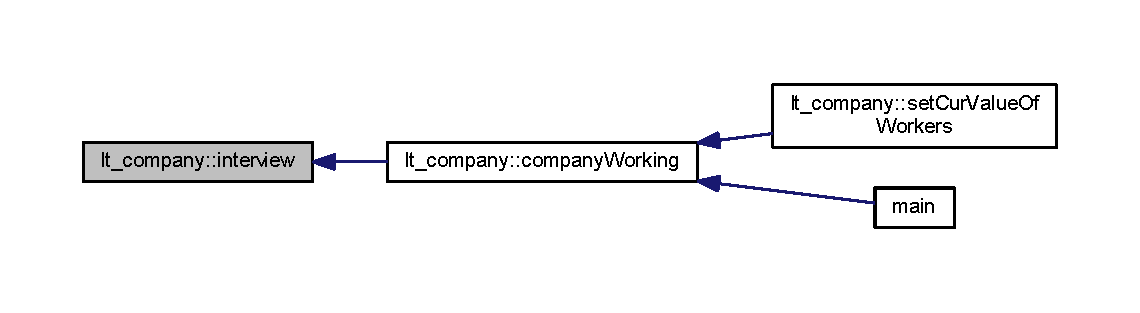
\includegraphics[width=350pt]{class_it__company_a0d05d1b25d00b221bbb66e57332dea08_icgraph}
\end{center}
\end{figure}
\hypertarget{class_it__company_ae83add85a00be1e24cdce48aa72678de}{}\label{class_it__company_ae83add85a00be1e24cdce48aa72678de} 
\index{It\+\_\+company@{It\+\_\+company}!operator++@{operator++}}
\index{operator++@{operator++}!It\+\_\+company@{It\+\_\+company}}
\subsubsection{\texorpdfstring{operator++()}{operator++()}}
{\footnotesize\ttfamily \hyperlink{class_it__company}{It\+\_\+company} \& It\+\_\+company\+::operator++ (\begin{DoxyParamCaption}{ }\end{DoxyParamCaption})}

Here is the call graph for this function\+:
\nopagebreak
\begin{figure}[H]
\begin{center}
\leavevmode
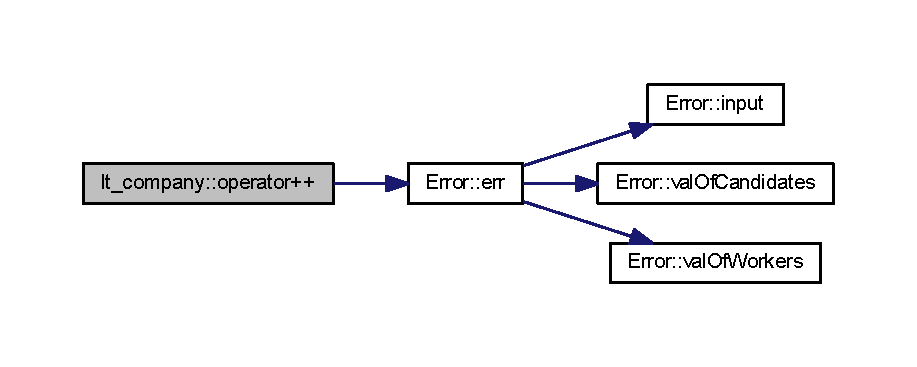
\includegraphics[width=350pt]{class_it__company_ae83add85a00be1e24cdce48aa72678de_cgraph}
\end{center}
\end{figure}
Here is the caller graph for this function\+:
\nopagebreak
\begin{figure}[H]
\begin{center}
\leavevmode
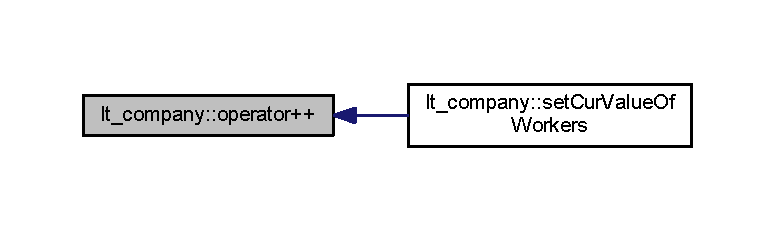
\includegraphics[width=350pt]{class_it__company_ae83add85a00be1e24cdce48aa72678de_icgraph}
\end{center}
\end{figure}
\hypertarget{class_it__company_ab5f464351646bc6458640391f5eab298}{}\label{class_it__company_ab5f464351646bc6458640391f5eab298} 
\index{It\+\_\+company@{It\+\_\+company}!preparing\+Vacancies\+And\+Tests@{preparing\+Vacancies\+And\+Tests}}
\index{preparing\+Vacancies\+And\+Tests@{preparing\+Vacancies\+And\+Tests}!It\+\_\+company@{It\+\_\+company}}
\subsubsection{\texorpdfstring{preparing\+Vacancies\+And\+Tests()}{preparingVacanciesAndTests()}}
{\footnotesize\ttfamily void It\+\_\+company\+::preparing\+Vacancies\+And\+Tests (\begin{DoxyParamCaption}{ }\end{DoxyParamCaption})\hspace{0.3cm}{\ttfamily [private]}}

Here is the call graph for this function\+:
\nopagebreak
\begin{figure}[H]
\begin{center}
\leavevmode
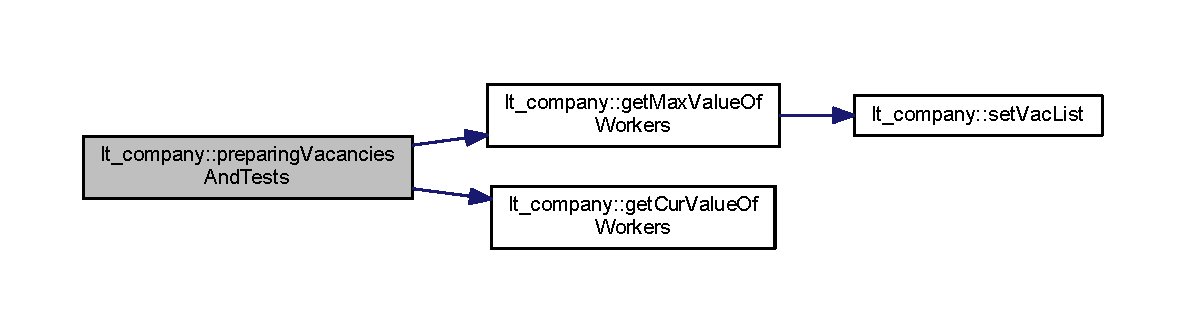
\includegraphics[width=350pt]{class_it__company_ab5f464351646bc6458640391f5eab298_cgraph}
\end{center}
\end{figure}
Here is the caller graph for this function\+:
\nopagebreak
\begin{figure}[H]
\begin{center}
\leavevmode
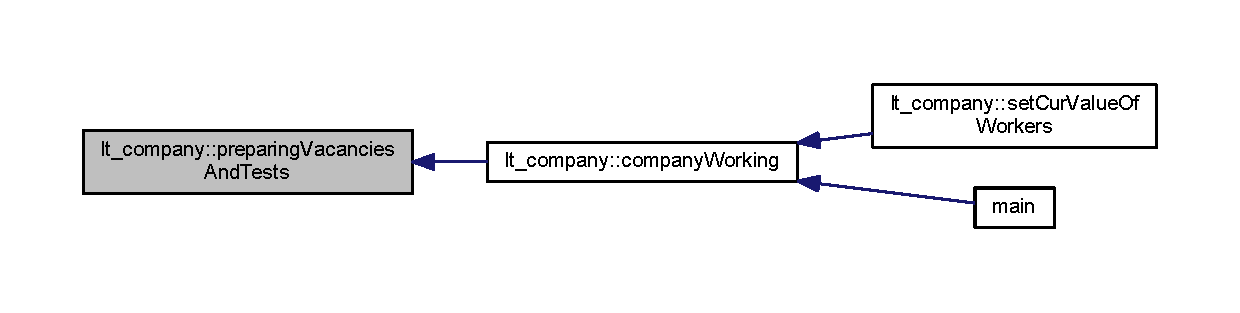
\includegraphics[width=350pt]{class_it__company_ab5f464351646bc6458640391f5eab298_icgraph}
\end{center}
\end{figure}
\hypertarget{class_it__company_ae06d651e9611d19f02bc1c7f29f2e988}{}\label{class_it__company_ae06d651e9611d19f02bc1c7f29f2e988} 
\index{It\+\_\+company@{It\+\_\+company}!set\+Cur\+Value\+Of\+Workers@{set\+Cur\+Value\+Of\+Workers}}
\index{set\+Cur\+Value\+Of\+Workers@{set\+Cur\+Value\+Of\+Workers}!It\+\_\+company@{It\+\_\+company}}
\subsubsection{\texorpdfstring{set\+Cur\+Value\+Of\+Workers()}{setCurValueOfWorkers()}}
{\footnotesize\ttfamily void It\+\_\+company\+::set\+Cur\+Value\+Of\+Workers (\begin{DoxyParamCaption}\item[{int}]{cur }\end{DoxyParamCaption})\hspace{0.3cm}{\ttfamily [inline]}}

Here is the call graph for this function\+:
\nopagebreak
\begin{figure}[H]
\begin{center}
\leavevmode
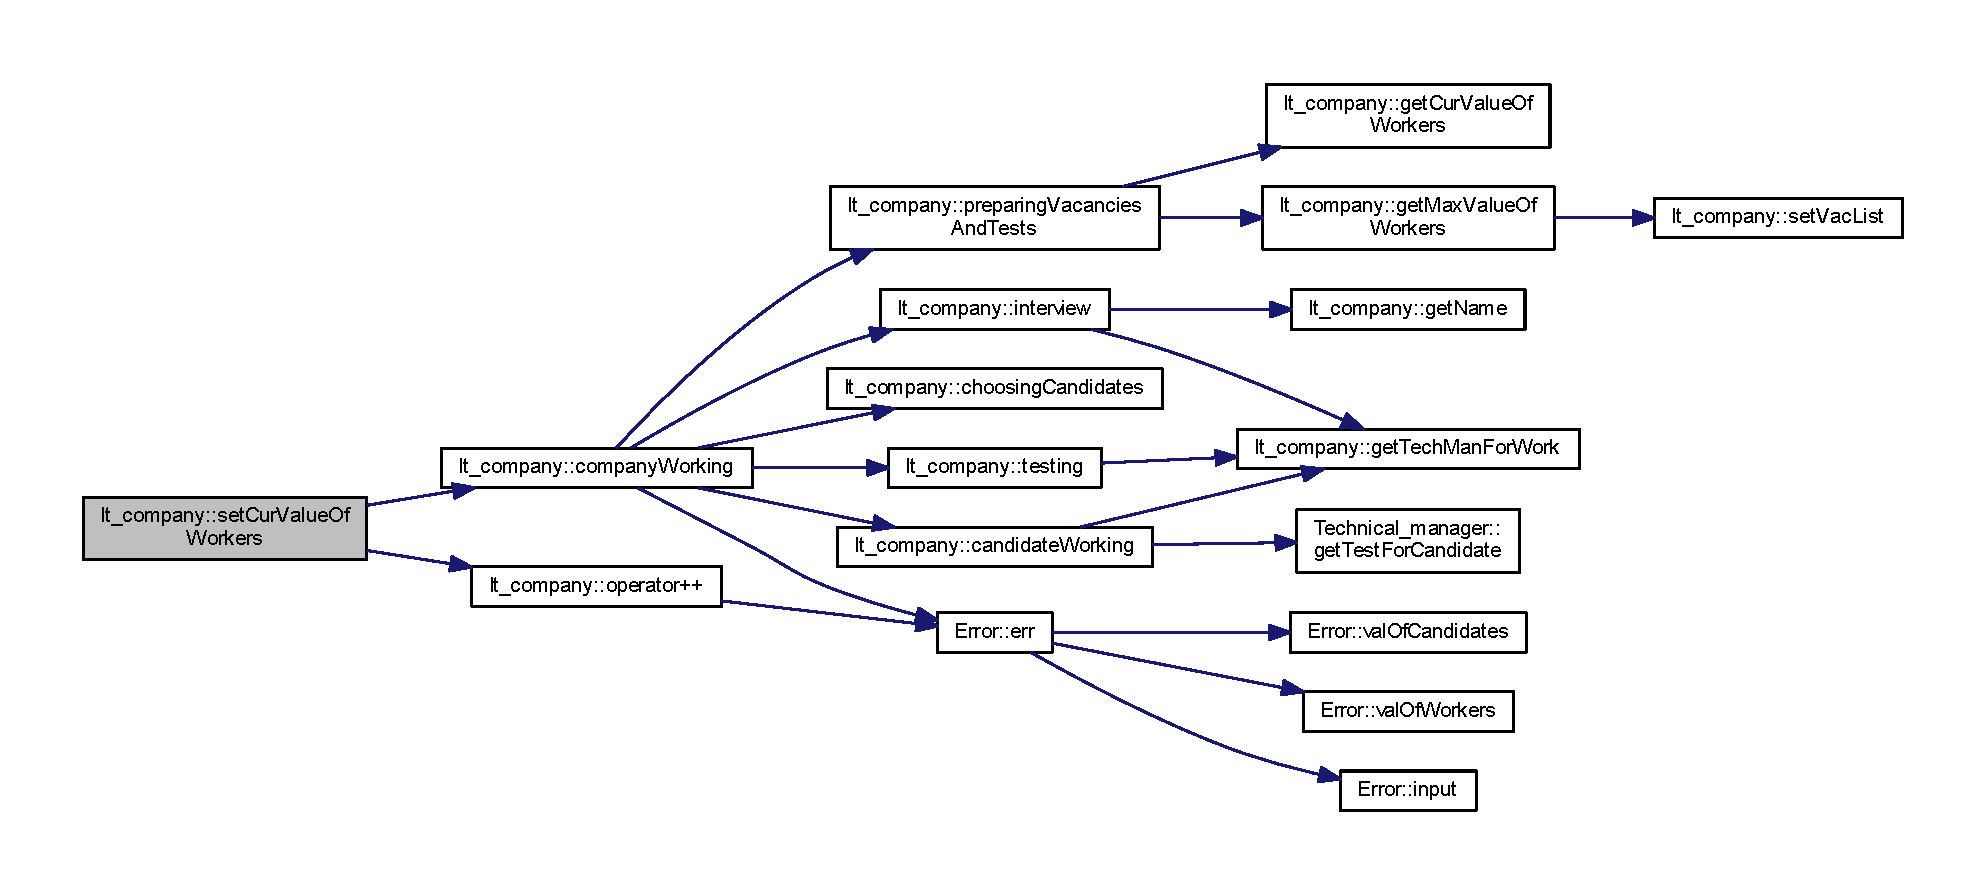
\includegraphics[width=350pt]{class_it__company_ae06d651e9611d19f02bc1c7f29f2e988_cgraph}
\end{center}
\end{figure}
\hypertarget{class_it__company_a079be9a566c94860e31acdb0c2953536}{}\label{class_it__company_a079be9a566c94860e31acdb0c2953536} 
\index{It\+\_\+company@{It\+\_\+company}!set\+Vac\+List@{set\+Vac\+List}}
\index{set\+Vac\+List@{set\+Vac\+List}!It\+\_\+company@{It\+\_\+company}}
\subsubsection{\texorpdfstring{set\+Vac\+List()}{setVacList()}}
{\footnotesize\ttfamily void It\+\_\+company\+::set\+Vac\+List (\begin{DoxyParamCaption}\item[{std\+::vector$<$ std\+::string $>$}]{vl }\end{DoxyParamCaption})}

Here is the caller graph for this function\+:
\nopagebreak
\begin{figure}[H]
\begin{center}
\leavevmode
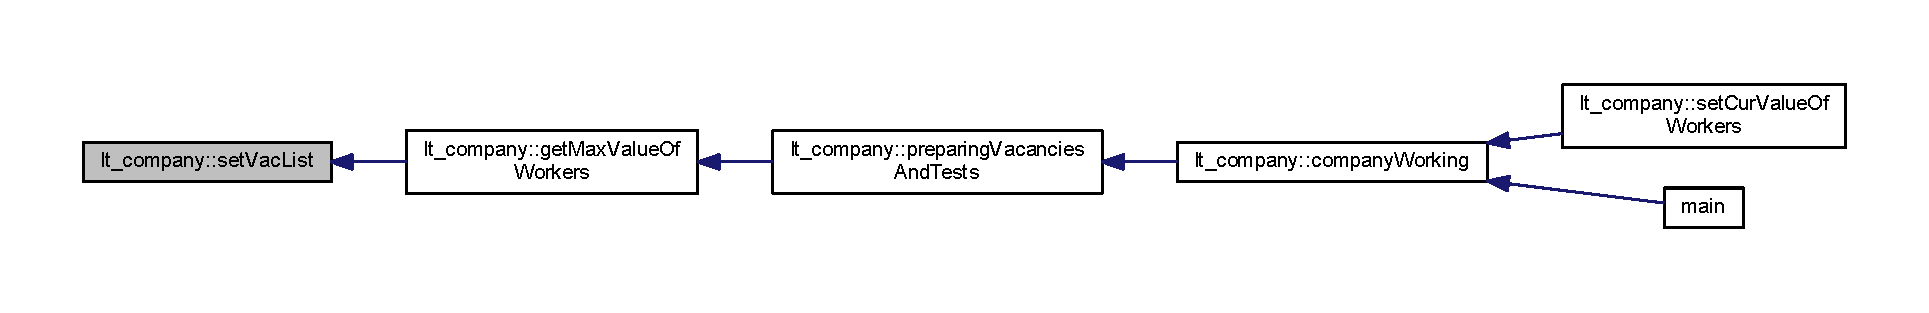
\includegraphics[width=350pt]{class_it__company_a079be9a566c94860e31acdb0c2953536_icgraph}
\end{center}
\end{figure}
\hypertarget{class_it__company_a2c7a94d7f82fb700c0d1f369423ad45f}{}\label{class_it__company_a2c7a94d7f82fb700c0d1f369423ad45f} 
\index{It\+\_\+company@{It\+\_\+company}!testing@{testing}}
\index{testing@{testing}!It\+\_\+company@{It\+\_\+company}}
\subsubsection{\texorpdfstring{testing()}{testing()}}
{\footnotesize\ttfamily void It\+\_\+company\+::testing (\begin{DoxyParamCaption}\item[{std\+::vector$<$ std\+::vector$<$ std\+::string $>$$>$ \&}]{all\+Answers,  }\item[{std\+::multimap$<$ int, int $>$ \&}]{cand\+Index }\end{DoxyParamCaption})\hspace{0.3cm}{\ttfamily [private]}}

Here is the call graph for this function\+:
\nopagebreak
\begin{figure}[H]
\begin{center}
\leavevmode
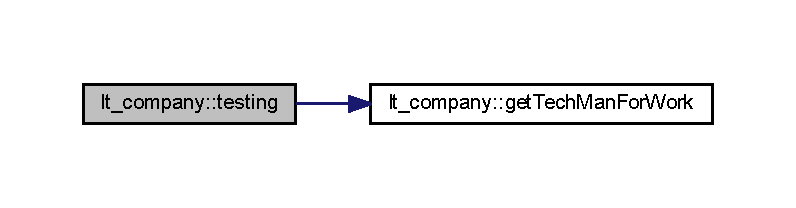
\includegraphics[width=350pt]{class_it__company_a2c7a94d7f82fb700c0d1f369423ad45f_cgraph}
\end{center}
\end{figure}
Here is the caller graph for this function\+:
\nopagebreak
\begin{figure}[H]
\begin{center}
\leavevmode
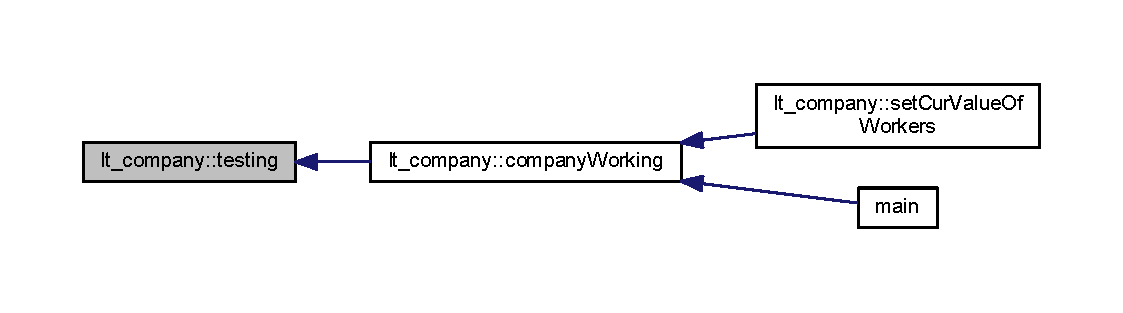
\includegraphics[width=350pt]{class_it__company_a2c7a94d7f82fb700c0d1f369423ad45f_icgraph}
\end{center}
\end{figure}


\subsection{Friends And Related Function Documentation}
\hypertarget{class_it__company_a962e1dda6d2c3075501e63a8d62693f7}{}\label{class_it__company_a962e1dda6d2c3075501e63a8d62693f7} 
\index{It\+\_\+company@{It\+\_\+company}!operator$<$$<$@{operator$<$$<$}}
\index{operator$<$$<$@{operator$<$$<$}!It\+\_\+company@{It\+\_\+company}}
\subsubsection{\texorpdfstring{operator$<$$<$}{operator<<}}
{\footnotesize\ttfamily std\+::ostream\& operator$<$$<$ (\begin{DoxyParamCaption}\item[{std\+::ostream \&}]{stream,  }\item[{\hyperlink{class_it__company}{It\+\_\+company}}]{itcompany }\end{DoxyParamCaption})\hspace{0.3cm}{\ttfamily [friend]}}



\subsection{Member Data Documentation}
\hypertarget{class_it__company_ac48dbef2db2cad83837c89efdc69b9c9}{}\label{class_it__company_ac48dbef2db2cad83837c89efdc69b9c9} 
\index{It\+\_\+company@{It\+\_\+company}!cur\+Value\+Of\+Workers@{cur\+Value\+Of\+Workers}}
\index{cur\+Value\+Of\+Workers@{cur\+Value\+Of\+Workers}!It\+\_\+company@{It\+\_\+company}}
\subsubsection{\texorpdfstring{cur\+Value\+Of\+Workers}{curValueOfWorkers}}
{\footnotesize\ttfamily int It\+\_\+company\+::cur\+Value\+Of\+Workers\hspace{0.3cm}{\ttfamily [private]}}

\hypertarget{class_it__company_ae0e3f81754b1433c6dfb5ebe96f620d1}{}\label{class_it__company_ae0e3f81754b1433c6dfb5ebe96f620d1} 
\index{It\+\_\+company@{It\+\_\+company}!hr\+\_\+manager@{hr\+\_\+manager}}
\index{hr\+\_\+manager@{hr\+\_\+manager}!It\+\_\+company@{It\+\_\+company}}
\subsubsection{\texorpdfstring{hr\+\_\+manager}{hr\_manager}}
{\footnotesize\ttfamily std\+::vector$<$\hyperlink{class_hr__manager}{Hr\+\_\+manager}$>$ It\+\_\+company\+::hr\+\_\+manager}

\hypertarget{class_it__company_ac71fd3642622747e9e543b5a193ba525}{}\label{class_it__company_ac71fd3642622747e9e543b5a193ba525} 
\index{It\+\_\+company@{It\+\_\+company}!max\+Value\+Of\+Workers@{max\+Value\+Of\+Workers}}
\index{max\+Value\+Of\+Workers@{max\+Value\+Of\+Workers}!It\+\_\+company@{It\+\_\+company}}
\subsubsection{\texorpdfstring{max\+Value\+Of\+Workers}{maxValueOfWorkers}}
{\footnotesize\ttfamily const int It\+\_\+company\+::max\+Value\+Of\+Workers = 3\hspace{0.3cm}{\ttfamily [static]}, {\ttfamily [private]}}

\hypertarget{class_it__company_a99894304639dab6b416f697dc7e81d52}{}\label{class_it__company_a99894304639dab6b416f697dc7e81d52} 
\index{It\+\_\+company@{It\+\_\+company}!name@{name}}
\index{name@{name}!It\+\_\+company@{It\+\_\+company}}
\subsubsection{\texorpdfstring{name}{name}}
{\footnotesize\ttfamily const std\+::string It\+\_\+company\+::name\hspace{0.3cm}{\ttfamily [private]}}

\hypertarget{class_it__company_af2285094fb07bcf0a9f3a4c1d8a407d3}{}\label{class_it__company_af2285094fb07bcf0a9f3a4c1d8a407d3} 
\index{It\+\_\+company@{It\+\_\+company}!technical\+\_\+manager@{technical\+\_\+manager}}
\index{technical\+\_\+manager@{technical\+\_\+manager}!It\+\_\+company@{It\+\_\+company}}
\subsubsection{\texorpdfstring{technical\+\_\+manager}{technical\_manager}}
{\footnotesize\ttfamily std\+::vector$<$\hyperlink{class_technical__manager}{Technical\+\_\+manager}$>$ It\+\_\+company\+::technical\+\_\+manager}

\hypertarget{class_it__company_a06d700346a5bcd94c1f265f3bb65143f}{}\label{class_it__company_a06d700346a5bcd94c1f265f3bb65143f} 
\index{It\+\_\+company@{It\+\_\+company}!vacancy\+List@{vacancy\+List}}
\index{vacancy\+List@{vacancy\+List}!It\+\_\+company@{It\+\_\+company}}
\subsubsection{\texorpdfstring{vacancy\+List}{vacancyList}}
{\footnotesize\ttfamily std\+::vector$<$std\+::string$>$ It\+\_\+company\+::vacancy\+List\hspace{0.3cm}{\ttfamily [private]}}



The documentation for this class was generated from the following files\+:\begin{DoxyCompactItemize}
\item 
\hyperlink{_it__company_8h}{It\+\_\+company.\+h}\item 
\hyperlink{_it__company_8cpp}{It\+\_\+company.\+cpp}\end{DoxyCompactItemize}

\hypertarget{class_resume}{}\section{Resume Class Reference}
\label{class_resume}\index{Resume@{Resume}}


{\ttfamily \#include $<$Resume.\+h$>$}



Collaboration diagram for Resume\+:
\nopagebreak
\begin{figure}[H]
\begin{center}
\leavevmode
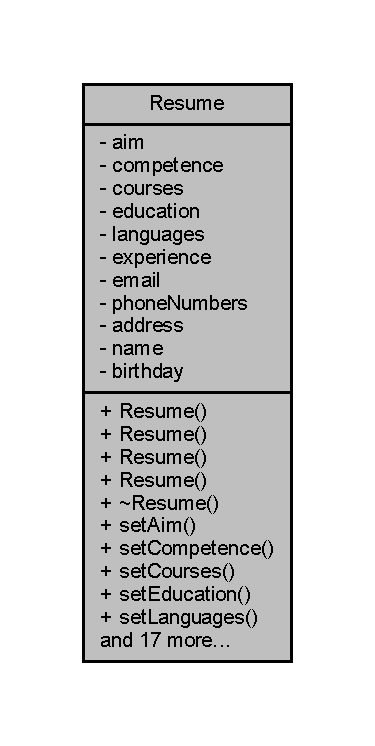
\includegraphics[width=180pt]{class_resume__coll__graph}
\end{center}
\end{figure}
\subsection*{Public Member Functions}
\begin{DoxyCompactItemize}
\item 
\hyperlink{class_resume_a71d23f61d7eb1560a918f6b3bf65fdc5}{Resume} ()
\item 
\hyperlink{class_resume_a92600ef21027117b53ab9d3fdb6705f5}{Resume} (std\+::string \hyperlink{class_resume_ace4b574b42cdc210ed457987c045410a}{aim}, std\+::string comp, std\+::vector$<$ std\+::string $>$ \hyperlink{class_resume_afae66c6c6d6c04b721dce001d25e2d35}{courses}, std\+::string educ, std\+::vector$<$ std\+::string $>$ lang, int exp, std\+::string \hyperlink{class_resume_a376e6779f0f414aec00ca78c36dd1c2a}{email}, std\+::vector$<$ int $>$ phone, std\+::string \hyperlink{class_resume_a31098a2b61a35edbf3c6a525235e5976}{address}, std\+::string \hyperlink{class_resume_ae99dd9e5aa53753a02b105478a76214a}{name}, std\+::string birth)
\item 
\hyperlink{class_resume_a6fc2de3d11d4650dd7720c344386c8a2}{Resume} (\hyperlink{class_resume}{Resume} \&s\+Resume)
\item 
\hyperlink{class_resume_a0da0b86ce16756cdfe0cc34afa77e975}{Resume} (std\+::string str)
\item 
\hyperlink{class_resume_a86b302420dc26041de719f14ce6e6621}{$\sim$\+Resume} ()
\item 
void \hyperlink{class_resume_a48d6e397c93b741a2fe96ba83f36c40f}{set\+Aim} (std\+::string a)
\item 
void \hyperlink{class_resume_adce5a6624de56751c72f8fe2989da5c9}{set\+Competence} (std\+::string c)
\item 
void \hyperlink{class_resume_a2a80b2496ae5bfbf456f4fe6170b9a21}{set\+Courses} (std\+::vector$<$ std\+::string $>$ c)
\item 
void \hyperlink{class_resume_a9a76b4b2d010ce5259b9be3ff9fca2b6}{set\+Education} (std\+::string e)
\item 
void \hyperlink{class_resume_ae51fc034e53ba1118f3d49b3bd0b1e0f}{set\+Languages} (std\+::vector$<$ std\+::string $>$ l)
\item 
void \hyperlink{class_resume_a3742ddd777e93ad124560cec7da409fa}{set\+Experience} (int exp)
\item 
void \hyperlink{class_resume_a35e1a0db9143d3fcdce851c2156b9060}{set\+Email} (std\+::string mail)
\item 
void \hyperlink{class_resume_a97ea87081895f4319f72aec9a3f4fd1c}{set\+Phones} (std\+::vector$<$ int $>$ p)
\item 
void \hyperlink{class_resume_a03adc6528b2ed6302008a249109005a8}{set\+Address} (std\+::string ad)
\item 
void \hyperlink{class_resume_a47a244bcf3498360be01b98c8773c847}{set\+Name} (std\+::string n)
\item 
void \hyperlink{class_resume_abc51f92eaaab42d9973693424147a421}{set\+Birthday} (std\+::string b)
\item 
std\+::string \hyperlink{class_resume_a65f42d7448ffe5ecdbc33663ad9339e0}{get\+Aim} (void) const
\item 
std\+::string \hyperlink{class_resume_afd0ba86a30b73693a6eda28c9ecf7860}{get\+Competence} (void) const
\item 
std\+::vector$<$ std\+::string $>$ \hyperlink{class_resume_ac4c445be5628971ce45ab02213e6769f}{get\+Courses} (void) const
\item 
std\+::string \hyperlink{class_resume_af57d4658748a7e718d546594bfd74450}{get\+Education} (void) const
\item 
std\+::vector$<$ std\+::string $>$ \hyperlink{class_resume_a48cfbd4c9c8a100deb4656b7f83402cc}{get\+Languages} (void) const
\item 
int \hyperlink{class_resume_ad8abe2f52e3a5b4f730c87ab297ea99a}{get\+Experience} (void) const
\item 
std\+::string \hyperlink{class_resume_af38cb080447a7c96b20026999fd330ee}{get\+Email} (void) const
\item 
std\+::vector$<$ int $>$ \hyperlink{class_resume_a3ca8f1b8a98de8dfe7ac3897f2577ca2}{get\+Phones} (void) const
\item 
std\+::string \hyperlink{class_resume_af11a5f3bfadd89987d4603190647a89d}{get\+Address} (void) const
\item 
std\+::string \hyperlink{class_resume_a7e20376daab81badef8a7edfa1f422d8}{get\+Name} (void) const
\item 
std\+::string \hyperlink{class_resume_a68cfeeffdaa6cb63701593b2c086d274}{get\+Birthday} (void) const
\end{DoxyCompactItemize}
\subsection*{Private Attributes}
\begin{DoxyCompactItemize}
\item 
std\+::string \hyperlink{class_resume_ace4b574b42cdc210ed457987c045410a}{aim}
\item 
std\+::string \hyperlink{class_resume_ac537d9f0cdc7dd3cb87f9d32d7653d22}{competence}
\item 
std\+::vector$<$ std\+::string $>$ \hyperlink{class_resume_afae66c6c6d6c04b721dce001d25e2d35}{courses}
\item 
std\+::string \hyperlink{class_resume_a60f48cd7a2bb8a9dc44ab62bf8b55231}{education}
\item 
std\+::vector$<$ std\+::string $>$ \hyperlink{class_resume_a4035be2ef3fb8fbdaf60ea05ef0868c3}{languages}
\item 
int \hyperlink{class_resume_af49c8b6d88d53bc168c7abd595b3faf9}{experience}
\item 
std\+::string \hyperlink{class_resume_a376e6779f0f414aec00ca78c36dd1c2a}{email}
\item 
std\+::vector$<$ int $>$ \hyperlink{class_resume_a82cc5431107459a181378b8ce3fbbb0d}{phone\+Numbers}
\item 
std\+::string \hyperlink{class_resume_a31098a2b61a35edbf3c6a525235e5976}{address}
\item 
std\+::string \hyperlink{class_resume_ae99dd9e5aa53753a02b105478a76214a}{name}
\item 
std\+::string \hyperlink{class_resume_a0cfd6d3cfb1a1ce4409e24efb00c9eb1}{birthday}
\end{DoxyCompactItemize}
\subsection*{Friends}
\begin{DoxyCompactItemize}
\item 
std\+::ostream \& \hyperlink{class_resume_a4802836099b1fa0441f74d081cd39cf2}{operator$<$$<$} (std\+::ostream \&stream, \hyperlink{class_resume}{Resume} resume)
\item 
std\+::ostream \& \hyperlink{class_resume_a3e74504543874fb381d00e0e9444d85f}{operator$>$$>$} (std\+::ostream \&stream, \hyperlink{class_resume}{Resume} resume)
\end{DoxyCompactItemize}


\subsection{Constructor \& Destructor Documentation}
\hypertarget{class_resume_a71d23f61d7eb1560a918f6b3bf65fdc5}{}\label{class_resume_a71d23f61d7eb1560a918f6b3bf65fdc5} 
\index{Resume@{Resume}!Resume@{Resume}}
\index{Resume@{Resume}!Resume@{Resume}}
\subsubsection{\texorpdfstring{Resume()}{Resume()}\hspace{0.1cm}{\footnotesize\ttfamily [1/4]}}
{\footnotesize\ttfamily Resume\+::\+Resume (\begin{DoxyParamCaption}{ }\end{DoxyParamCaption})}

\hypertarget{class_resume_a92600ef21027117b53ab9d3fdb6705f5}{}\label{class_resume_a92600ef21027117b53ab9d3fdb6705f5} 
\index{Resume@{Resume}!Resume@{Resume}}
\index{Resume@{Resume}!Resume@{Resume}}
\subsubsection{\texorpdfstring{Resume()}{Resume()}\hspace{0.1cm}{\footnotesize\ttfamily [2/4]}}
{\footnotesize\ttfamily Resume\+::\+Resume (\begin{DoxyParamCaption}\item[{std\+::string}]{aim,  }\item[{std\+::string}]{comp,  }\item[{std\+::vector$<$ std\+::string $>$}]{courses,  }\item[{std\+::string}]{educ,  }\item[{std\+::vector$<$ std\+::string $>$}]{lang,  }\item[{int}]{exp,  }\item[{std\+::string}]{email,  }\item[{std\+::vector$<$ int $>$}]{phone,  }\item[{std\+::string}]{address,  }\item[{std\+::string}]{name,  }\item[{std\+::string}]{birth }\end{DoxyParamCaption})}

\hypertarget{class_resume_a6fc2de3d11d4650dd7720c344386c8a2}{}\label{class_resume_a6fc2de3d11d4650dd7720c344386c8a2} 
\index{Resume@{Resume}!Resume@{Resume}}
\index{Resume@{Resume}!Resume@{Resume}}
\subsubsection{\texorpdfstring{Resume()}{Resume()}\hspace{0.1cm}{\footnotesize\ttfamily [3/4]}}
{\footnotesize\ttfamily Resume\+::\+Resume (\begin{DoxyParamCaption}\item[{\hyperlink{class_resume}{Resume} \&}]{s\+Resume }\end{DoxyParamCaption})}

\hypertarget{class_resume_a0da0b86ce16756cdfe0cc34afa77e975}{}\label{class_resume_a0da0b86ce16756cdfe0cc34afa77e975} 
\index{Resume@{Resume}!Resume@{Resume}}
\index{Resume@{Resume}!Resume@{Resume}}
\subsubsection{\texorpdfstring{Resume()}{Resume()}\hspace{0.1cm}{\footnotesize\ttfamily [4/4]}}
{\footnotesize\ttfamily Resume\+::\+Resume (\begin{DoxyParamCaption}\item[{std\+::string}]{str }\end{DoxyParamCaption})}

\hypertarget{class_resume_a86b302420dc26041de719f14ce6e6621}{}\label{class_resume_a86b302420dc26041de719f14ce6e6621} 
\index{Resume@{Resume}!````~Resume@{$\sim$\+Resume}}
\index{````~Resume@{$\sim$\+Resume}!Resume@{Resume}}
\subsubsection{\texorpdfstring{$\sim$\+Resume()}{~Resume()}}
{\footnotesize\ttfamily Resume\+::$\sim$\+Resume (\begin{DoxyParamCaption}{ }\end{DoxyParamCaption})\hspace{0.3cm}{\ttfamily [inline]}}

Here is the call graph for this function\+:
\nopagebreak
\begin{figure}[H]
\begin{center}
\leavevmode
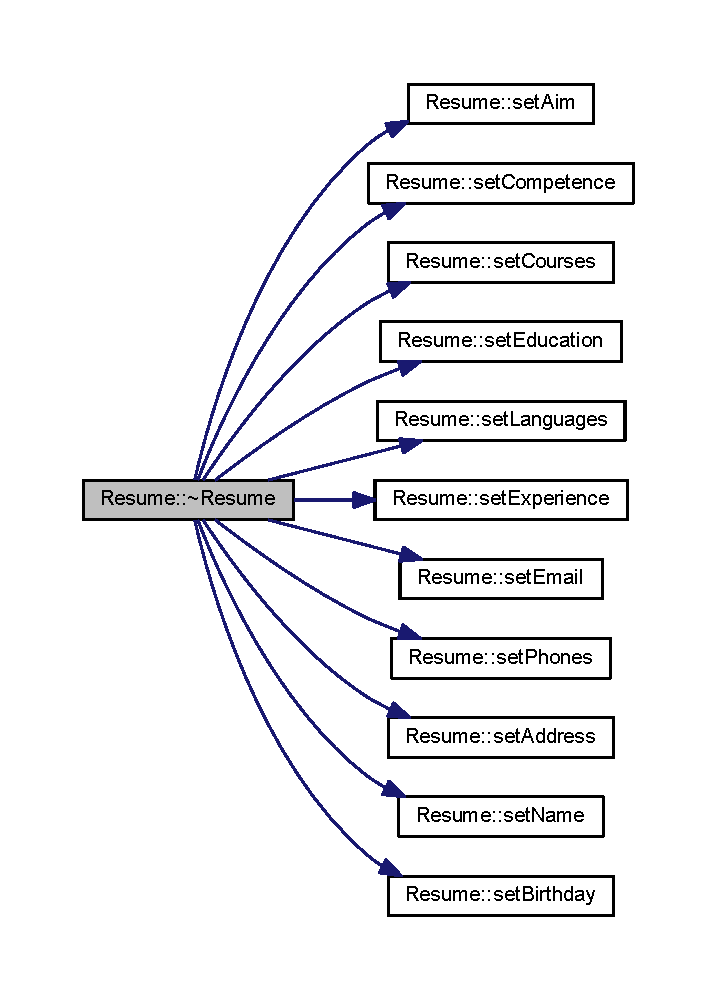
\includegraphics[width=344pt]{class_resume_a86b302420dc26041de719f14ce6e6621_cgraph}
\end{center}
\end{figure}


\subsection{Member Function Documentation}
\hypertarget{class_resume_af11a5f3bfadd89987d4603190647a89d}{}\label{class_resume_af11a5f3bfadd89987d4603190647a89d} 
\index{Resume@{Resume}!get\+Address@{get\+Address}}
\index{get\+Address@{get\+Address}!Resume@{Resume}}
\subsubsection{\texorpdfstring{get\+Address()}{getAddress()}}
{\footnotesize\ttfamily std\+::string Resume\+::get\+Address (\begin{DoxyParamCaption}\item[{void}]{ }\end{DoxyParamCaption}) const\hspace{0.3cm}{\ttfamily [inline]}}

\hypertarget{class_resume_a65f42d7448ffe5ecdbc33663ad9339e0}{}\label{class_resume_a65f42d7448ffe5ecdbc33663ad9339e0} 
\index{Resume@{Resume}!get\+Aim@{get\+Aim}}
\index{get\+Aim@{get\+Aim}!Resume@{Resume}}
\subsubsection{\texorpdfstring{get\+Aim()}{getAim()}}
{\footnotesize\ttfamily std\+::string Resume\+::get\+Aim (\begin{DoxyParamCaption}\item[{void}]{ }\end{DoxyParamCaption}) const\hspace{0.3cm}{\ttfamily [inline]}}

\hypertarget{class_resume_a68cfeeffdaa6cb63701593b2c086d274}{}\label{class_resume_a68cfeeffdaa6cb63701593b2c086d274} 
\index{Resume@{Resume}!get\+Birthday@{get\+Birthday}}
\index{get\+Birthday@{get\+Birthday}!Resume@{Resume}}
\subsubsection{\texorpdfstring{get\+Birthday()}{getBirthday()}}
{\footnotesize\ttfamily std\+::string Resume\+::get\+Birthday (\begin{DoxyParamCaption}\item[{void}]{ }\end{DoxyParamCaption}) const\hspace{0.3cm}{\ttfamily [inline]}}

\hypertarget{class_resume_afd0ba86a30b73693a6eda28c9ecf7860}{}\label{class_resume_afd0ba86a30b73693a6eda28c9ecf7860} 
\index{Resume@{Resume}!get\+Competence@{get\+Competence}}
\index{get\+Competence@{get\+Competence}!Resume@{Resume}}
\subsubsection{\texorpdfstring{get\+Competence()}{getCompetence()}}
{\footnotesize\ttfamily std\+::string Resume\+::get\+Competence (\begin{DoxyParamCaption}\item[{void}]{ }\end{DoxyParamCaption}) const\hspace{0.3cm}{\ttfamily [inline]}}

\hypertarget{class_resume_ac4c445be5628971ce45ab02213e6769f}{}\label{class_resume_ac4c445be5628971ce45ab02213e6769f} 
\index{Resume@{Resume}!get\+Courses@{get\+Courses}}
\index{get\+Courses@{get\+Courses}!Resume@{Resume}}
\subsubsection{\texorpdfstring{get\+Courses()}{getCourses()}}
{\footnotesize\ttfamily std\+::vector$<$std\+::string$>$ Resume\+::get\+Courses (\begin{DoxyParamCaption}\item[{void}]{ }\end{DoxyParamCaption}) const\hspace{0.3cm}{\ttfamily [inline]}}

\hypertarget{class_resume_af57d4658748a7e718d546594bfd74450}{}\label{class_resume_af57d4658748a7e718d546594bfd74450} 
\index{Resume@{Resume}!get\+Education@{get\+Education}}
\index{get\+Education@{get\+Education}!Resume@{Resume}}
\subsubsection{\texorpdfstring{get\+Education()}{getEducation()}}
{\footnotesize\ttfamily std\+::string Resume\+::get\+Education (\begin{DoxyParamCaption}\item[{void}]{ }\end{DoxyParamCaption}) const\hspace{0.3cm}{\ttfamily [inline]}}

\hypertarget{class_resume_af38cb080447a7c96b20026999fd330ee}{}\label{class_resume_af38cb080447a7c96b20026999fd330ee} 
\index{Resume@{Resume}!get\+Email@{get\+Email}}
\index{get\+Email@{get\+Email}!Resume@{Resume}}
\subsubsection{\texorpdfstring{get\+Email()}{getEmail()}}
{\footnotesize\ttfamily std\+::string Resume\+::get\+Email (\begin{DoxyParamCaption}\item[{void}]{ }\end{DoxyParamCaption}) const\hspace{0.3cm}{\ttfamily [inline]}}

\hypertarget{class_resume_ad8abe2f52e3a5b4f730c87ab297ea99a}{}\label{class_resume_ad8abe2f52e3a5b4f730c87ab297ea99a} 
\index{Resume@{Resume}!get\+Experience@{get\+Experience}}
\index{get\+Experience@{get\+Experience}!Resume@{Resume}}
\subsubsection{\texorpdfstring{get\+Experience()}{getExperience()}}
{\footnotesize\ttfamily int Resume\+::get\+Experience (\begin{DoxyParamCaption}\item[{void}]{ }\end{DoxyParamCaption}) const\hspace{0.3cm}{\ttfamily [inline]}}

Here is the caller graph for this function\+:
\nopagebreak
\begin{figure}[H]
\begin{center}
\leavevmode
\includegraphics[width=350pt]{class_resume_ad8abe2f52e3a5b4f730c87ab297ea99a_icgraph}
\end{center}
\end{figure}
\hypertarget{class_resume_a48cfbd4c9c8a100deb4656b7f83402cc}{}\label{class_resume_a48cfbd4c9c8a100deb4656b7f83402cc} 
\index{Resume@{Resume}!get\+Languages@{get\+Languages}}
\index{get\+Languages@{get\+Languages}!Resume@{Resume}}
\subsubsection{\texorpdfstring{get\+Languages()}{getLanguages()}}
{\footnotesize\ttfamily std\+::vector$<$std\+::string$>$ Resume\+::get\+Languages (\begin{DoxyParamCaption}\item[{void}]{ }\end{DoxyParamCaption}) const\hspace{0.3cm}{\ttfamily [inline]}}

\hypertarget{class_resume_a7e20376daab81badef8a7edfa1f422d8}{}\label{class_resume_a7e20376daab81badef8a7edfa1f422d8} 
\index{Resume@{Resume}!get\+Name@{get\+Name}}
\index{get\+Name@{get\+Name}!Resume@{Resume}}
\subsubsection{\texorpdfstring{get\+Name()}{getName()}}
{\footnotesize\ttfamily std\+::string Resume\+::get\+Name (\begin{DoxyParamCaption}\item[{void}]{ }\end{DoxyParamCaption}) const\hspace{0.3cm}{\ttfamily [inline]}}

\hypertarget{class_resume_a3ca8f1b8a98de8dfe7ac3897f2577ca2}{}\label{class_resume_a3ca8f1b8a98de8dfe7ac3897f2577ca2} 
\index{Resume@{Resume}!get\+Phones@{get\+Phones}}
\index{get\+Phones@{get\+Phones}!Resume@{Resume}}
\subsubsection{\texorpdfstring{get\+Phones()}{getPhones()}}
{\footnotesize\ttfamily std\+::vector$<$int$>$ Resume\+::get\+Phones (\begin{DoxyParamCaption}\item[{void}]{ }\end{DoxyParamCaption}) const\hspace{0.3cm}{\ttfamily [inline]}}

\hypertarget{class_resume_a03adc6528b2ed6302008a249109005a8}{}\label{class_resume_a03adc6528b2ed6302008a249109005a8} 
\index{Resume@{Resume}!set\+Address@{set\+Address}}
\index{set\+Address@{set\+Address}!Resume@{Resume}}
\subsubsection{\texorpdfstring{set\+Address()}{setAddress()}}
{\footnotesize\ttfamily void Resume\+::set\+Address (\begin{DoxyParamCaption}\item[{std\+::string}]{ad }\end{DoxyParamCaption})}

Here is the caller graph for this function\+:
\nopagebreak
\begin{figure}[H]
\begin{center}
\leavevmode
\includegraphics[width=325pt]{class_resume_a03adc6528b2ed6302008a249109005a8_icgraph}
\end{center}
\end{figure}
\hypertarget{class_resume_a48d6e397c93b741a2fe96ba83f36c40f}{}\label{class_resume_a48d6e397c93b741a2fe96ba83f36c40f} 
\index{Resume@{Resume}!set\+Aim@{set\+Aim}}
\index{set\+Aim@{set\+Aim}!Resume@{Resume}}
\subsubsection{\texorpdfstring{set\+Aim()}{setAim()}}
{\footnotesize\ttfamily void Resume\+::set\+Aim (\begin{DoxyParamCaption}\item[{std\+::string}]{a }\end{DoxyParamCaption})}

Here is the caller graph for this function\+:
\nopagebreak
\begin{figure}[H]
\begin{center}
\leavevmode
\includegraphics[width=306pt]{class_resume_a48d6e397c93b741a2fe96ba83f36c40f_icgraph}
\end{center}
\end{figure}
\hypertarget{class_resume_abc51f92eaaab42d9973693424147a421}{}\label{class_resume_abc51f92eaaab42d9973693424147a421} 
\index{Resume@{Resume}!set\+Birthday@{set\+Birthday}}
\index{set\+Birthday@{set\+Birthday}!Resume@{Resume}}
\subsubsection{\texorpdfstring{set\+Birthday()}{setBirthday()}}
{\footnotesize\ttfamily void Resume\+::set\+Birthday (\begin{DoxyParamCaption}\item[{std\+::string}]{b }\end{DoxyParamCaption})}

Here is the caller graph for this function\+:
\nopagebreak
\begin{figure}[H]
\begin{center}
\leavevmode
\includegraphics[width=325pt]{class_resume_abc51f92eaaab42d9973693424147a421_icgraph}
\end{center}
\end{figure}
\hypertarget{class_resume_adce5a6624de56751c72f8fe2989da5c9}{}\label{class_resume_adce5a6624de56751c72f8fe2989da5c9} 
\index{Resume@{Resume}!set\+Competence@{set\+Competence}}
\index{set\+Competence@{set\+Competence}!Resume@{Resume}}
\subsubsection{\texorpdfstring{set\+Competence()}{setCompetence()}}
{\footnotesize\ttfamily void Resume\+::set\+Competence (\begin{DoxyParamCaption}\item[{std\+::string}]{c }\end{DoxyParamCaption})}

Here is the caller graph for this function\+:
\nopagebreak
\begin{figure}[H]
\begin{center}
\leavevmode
\includegraphics[width=350pt]{class_resume_adce5a6624de56751c72f8fe2989da5c9_icgraph}
\end{center}
\end{figure}
\hypertarget{class_resume_a2a80b2496ae5bfbf456f4fe6170b9a21}{}\label{class_resume_a2a80b2496ae5bfbf456f4fe6170b9a21} 
\index{Resume@{Resume}!set\+Courses@{set\+Courses}}
\index{set\+Courses@{set\+Courses}!Resume@{Resume}}
\subsubsection{\texorpdfstring{set\+Courses()}{setCourses()}}
{\footnotesize\ttfamily void Resume\+::set\+Courses (\begin{DoxyParamCaption}\item[{std\+::vector$<$ std\+::string $>$}]{c }\end{DoxyParamCaption})}

Here is the caller graph for this function\+:
\nopagebreak
\begin{figure}[H]
\begin{center}
\leavevmode
\includegraphics[width=325pt]{class_resume_a2a80b2496ae5bfbf456f4fe6170b9a21_icgraph}
\end{center}
\end{figure}
\hypertarget{class_resume_a9a76b4b2d010ce5259b9be3ff9fca2b6}{}\label{class_resume_a9a76b4b2d010ce5259b9be3ff9fca2b6} 
\index{Resume@{Resume}!set\+Education@{set\+Education}}
\index{set\+Education@{set\+Education}!Resume@{Resume}}
\subsubsection{\texorpdfstring{set\+Education()}{setEducation()}}
{\footnotesize\ttfamily void Resume\+::set\+Education (\begin{DoxyParamCaption}\item[{std\+::string}]{e }\end{DoxyParamCaption})}

Here is the caller graph for this function\+:
\nopagebreak
\begin{figure}[H]
\begin{center}
\leavevmode
\includegraphics[width=350pt]{class_resume_a9a76b4b2d010ce5259b9be3ff9fca2b6_icgraph}
\end{center}
\end{figure}
\hypertarget{class_resume_a35e1a0db9143d3fcdce851c2156b9060}{}\label{class_resume_a35e1a0db9143d3fcdce851c2156b9060} 
\index{Resume@{Resume}!set\+Email@{set\+Email}}
\index{set\+Email@{set\+Email}!Resume@{Resume}}
\subsubsection{\texorpdfstring{set\+Email()}{setEmail()}}
{\footnotesize\ttfamily void Resume\+::set\+Email (\begin{DoxyParamCaption}\item[{std\+::string}]{mail }\end{DoxyParamCaption})}

Here is the caller graph for this function\+:
\nopagebreak
\begin{figure}[H]
\begin{center}
\leavevmode
\includegraphics[width=314pt]{class_resume_a35e1a0db9143d3fcdce851c2156b9060_icgraph}
\end{center}
\end{figure}
\hypertarget{class_resume_a3742ddd777e93ad124560cec7da409fa}{}\label{class_resume_a3742ddd777e93ad124560cec7da409fa} 
\index{Resume@{Resume}!set\+Experience@{set\+Experience}}
\index{set\+Experience@{set\+Experience}!Resume@{Resume}}
\subsubsection{\texorpdfstring{set\+Experience()}{setExperience()}}
{\footnotesize\ttfamily void Resume\+::set\+Experience (\begin{DoxyParamCaption}\item[{int}]{exp }\end{DoxyParamCaption})}

Here is the caller graph for this function\+:
\nopagebreak
\begin{figure}[H]
\begin{center}
\leavevmode
\includegraphics[width=350pt]{class_resume_a3742ddd777e93ad124560cec7da409fa_icgraph}
\end{center}
\end{figure}
\hypertarget{class_resume_ae51fc034e53ba1118f3d49b3bd0b1e0f}{}\label{class_resume_ae51fc034e53ba1118f3d49b3bd0b1e0f} 
\index{Resume@{Resume}!set\+Languages@{set\+Languages}}
\index{set\+Languages@{set\+Languages}!Resume@{Resume}}
\subsubsection{\texorpdfstring{set\+Languages()}{setLanguages()}}
{\footnotesize\ttfamily void Resume\+::set\+Languages (\begin{DoxyParamCaption}\item[{std\+::vector$<$ std\+::string $>$}]{l }\end{DoxyParamCaption})}

Here is the caller graph for this function\+:
\nopagebreak
\begin{figure}[H]
\begin{center}
\leavevmode
\includegraphics[width=336pt]{class_resume_ae51fc034e53ba1118f3d49b3bd0b1e0f_icgraph}
\end{center}
\end{figure}
\hypertarget{class_resume_a47a244bcf3498360be01b98c8773c847}{}\label{class_resume_a47a244bcf3498360be01b98c8773c847} 
\index{Resume@{Resume}!set\+Name@{set\+Name}}
\index{set\+Name@{set\+Name}!Resume@{Resume}}
\subsubsection{\texorpdfstring{set\+Name()}{setName()}}
{\footnotesize\ttfamily void Resume\+::set\+Name (\begin{DoxyParamCaption}\item[{std\+::string}]{n }\end{DoxyParamCaption})}

Here is the caller graph for this function\+:
\nopagebreak
\begin{figure}[H]
\begin{center}
\leavevmode
\includegraphics[width=315pt]{class_resume_a47a244bcf3498360be01b98c8773c847_icgraph}
\end{center}
\end{figure}
\hypertarget{class_resume_a97ea87081895f4319f72aec9a3f4fd1c}{}\label{class_resume_a97ea87081895f4319f72aec9a3f4fd1c} 
\index{Resume@{Resume}!set\+Phones@{set\+Phones}}
\index{set\+Phones@{set\+Phones}!Resume@{Resume}}
\subsubsection{\texorpdfstring{set\+Phones()}{setPhones()}}
{\footnotesize\ttfamily void Resume\+::set\+Phones (\begin{DoxyParamCaption}\item[{std\+::vector$<$ int $>$}]{p }\end{DoxyParamCaption})}

Here is the caller graph for this function\+:
\nopagebreak
\begin{figure}[H]
\begin{center}
\leavevmode
\includegraphics[width=322pt]{class_resume_a97ea87081895f4319f72aec9a3f4fd1c_icgraph}
\end{center}
\end{figure}


\subsection{Friends And Related Function Documentation}
\hypertarget{class_resume_a4802836099b1fa0441f74d081cd39cf2}{}\label{class_resume_a4802836099b1fa0441f74d081cd39cf2} 
\index{Resume@{Resume}!operator$<$$<$@{operator$<$$<$}}
\index{operator$<$$<$@{operator$<$$<$}!Resume@{Resume}}
\subsubsection{\texorpdfstring{operator$<$$<$}{operator<<}}
{\footnotesize\ttfamily std\+::ostream\& operator$<$$<$ (\begin{DoxyParamCaption}\item[{std\+::ostream \&}]{stream,  }\item[{\hyperlink{class_resume}{Resume}}]{resume }\end{DoxyParamCaption})\hspace{0.3cm}{\ttfamily [friend]}}

\hypertarget{class_resume_a3e74504543874fb381d00e0e9444d85f}{}\label{class_resume_a3e74504543874fb381d00e0e9444d85f} 
\index{Resume@{Resume}!operator$>$$>$@{operator$>$$>$}}
\index{operator$>$$>$@{operator$>$$>$}!Resume@{Resume}}
\subsubsection{\texorpdfstring{operator$>$$>$}{operator>>}}
{\footnotesize\ttfamily std\+::ostream\& operator$>$$>$ (\begin{DoxyParamCaption}\item[{std\+::ostream \&}]{stream,  }\item[{\hyperlink{class_resume}{Resume}}]{resume }\end{DoxyParamCaption})\hspace{0.3cm}{\ttfamily [friend]}}



\subsection{Member Data Documentation}
\hypertarget{class_resume_a31098a2b61a35edbf3c6a525235e5976}{}\label{class_resume_a31098a2b61a35edbf3c6a525235e5976} 
\index{Resume@{Resume}!address@{address}}
\index{address@{address}!Resume@{Resume}}
\subsubsection{\texorpdfstring{address}{address}}
{\footnotesize\ttfamily std\+::string Resume\+::address\hspace{0.3cm}{\ttfamily [private]}}

\hypertarget{class_resume_ace4b574b42cdc210ed457987c045410a}{}\label{class_resume_ace4b574b42cdc210ed457987c045410a} 
\index{Resume@{Resume}!aim@{aim}}
\index{aim@{aim}!Resume@{Resume}}
\subsubsection{\texorpdfstring{aim}{aim}}
{\footnotesize\ttfamily std\+::string Resume\+::aim\hspace{0.3cm}{\ttfamily [private]}}

\hypertarget{class_resume_a0cfd6d3cfb1a1ce4409e24efb00c9eb1}{}\label{class_resume_a0cfd6d3cfb1a1ce4409e24efb00c9eb1} 
\index{Resume@{Resume}!birthday@{birthday}}
\index{birthday@{birthday}!Resume@{Resume}}
\subsubsection{\texorpdfstring{birthday}{birthday}}
{\footnotesize\ttfamily std\+::string Resume\+::birthday\hspace{0.3cm}{\ttfamily [private]}}

\hypertarget{class_resume_ac537d9f0cdc7dd3cb87f9d32d7653d22}{}\label{class_resume_ac537d9f0cdc7dd3cb87f9d32d7653d22} 
\index{Resume@{Resume}!competence@{competence}}
\index{competence@{competence}!Resume@{Resume}}
\subsubsection{\texorpdfstring{competence}{competence}}
{\footnotesize\ttfamily std\+::string Resume\+::competence\hspace{0.3cm}{\ttfamily [private]}}

\hypertarget{class_resume_afae66c6c6d6c04b721dce001d25e2d35}{}\label{class_resume_afae66c6c6d6c04b721dce001d25e2d35} 
\index{Resume@{Resume}!courses@{courses}}
\index{courses@{courses}!Resume@{Resume}}
\subsubsection{\texorpdfstring{courses}{courses}}
{\footnotesize\ttfamily std\+::vector$<$std\+::string$>$ Resume\+::courses\hspace{0.3cm}{\ttfamily [private]}}

\hypertarget{class_resume_a60f48cd7a2bb8a9dc44ab62bf8b55231}{}\label{class_resume_a60f48cd7a2bb8a9dc44ab62bf8b55231} 
\index{Resume@{Resume}!education@{education}}
\index{education@{education}!Resume@{Resume}}
\subsubsection{\texorpdfstring{education}{education}}
{\footnotesize\ttfamily std\+::string Resume\+::education\hspace{0.3cm}{\ttfamily [private]}}

\hypertarget{class_resume_a376e6779f0f414aec00ca78c36dd1c2a}{}\label{class_resume_a376e6779f0f414aec00ca78c36dd1c2a} 
\index{Resume@{Resume}!email@{email}}
\index{email@{email}!Resume@{Resume}}
\subsubsection{\texorpdfstring{email}{email}}
{\footnotesize\ttfamily std\+::string Resume\+::email\hspace{0.3cm}{\ttfamily [private]}}

\hypertarget{class_resume_af49c8b6d88d53bc168c7abd595b3faf9}{}\label{class_resume_af49c8b6d88d53bc168c7abd595b3faf9} 
\index{Resume@{Resume}!experience@{experience}}
\index{experience@{experience}!Resume@{Resume}}
\subsubsection{\texorpdfstring{experience}{experience}}
{\footnotesize\ttfamily int Resume\+::experience\hspace{0.3cm}{\ttfamily [private]}}

\hypertarget{class_resume_a4035be2ef3fb8fbdaf60ea05ef0868c3}{}\label{class_resume_a4035be2ef3fb8fbdaf60ea05ef0868c3} 
\index{Resume@{Resume}!languages@{languages}}
\index{languages@{languages}!Resume@{Resume}}
\subsubsection{\texorpdfstring{languages}{languages}}
{\footnotesize\ttfamily std\+::vector$<$std\+::string$>$ Resume\+::languages\hspace{0.3cm}{\ttfamily [private]}}

\hypertarget{class_resume_ae99dd9e5aa53753a02b105478a76214a}{}\label{class_resume_ae99dd9e5aa53753a02b105478a76214a} 
\index{Resume@{Resume}!name@{name}}
\index{name@{name}!Resume@{Resume}}
\subsubsection{\texorpdfstring{name}{name}}
{\footnotesize\ttfamily std\+::string Resume\+::name\hspace{0.3cm}{\ttfamily [private]}}

\hypertarget{class_resume_a82cc5431107459a181378b8ce3fbbb0d}{}\label{class_resume_a82cc5431107459a181378b8ce3fbbb0d} 
\index{Resume@{Resume}!phone\+Numbers@{phone\+Numbers}}
\index{phone\+Numbers@{phone\+Numbers}!Resume@{Resume}}
\subsubsection{\texorpdfstring{phone\+Numbers}{phoneNumbers}}
{\footnotesize\ttfamily std\+::vector$<$int$>$ Resume\+::phone\+Numbers\hspace{0.3cm}{\ttfamily [private]}}



The documentation for this class was generated from the following files\+:\begin{DoxyCompactItemize}
\item 
\hyperlink{_resume_8h}{Resume.\+h}\item 
\hyperlink{_resume_8cpp}{Resume.\+cpp}\end{DoxyCompactItemize}

\hypertarget{class_technical__manager}{}\section{Technical\+\_\+manager Class Reference}
\label{class_technical__manager}\index{Technical\+\_\+manager@{Technical\+\_\+manager}}


{\ttfamily \#include $<$Technical\+\_\+manager.\+h$>$}



Collaboration diagram for Technical\+\_\+manager\+:
\nopagebreak
\begin{figure}[H]
\begin{center}
\leavevmode
\includegraphics[width=202pt]{class_technical__manager__coll__graph}
\end{center}
\end{figure}
\subsection*{Public Member Functions}
\begin{DoxyCompactItemize}
\item 
\hyperlink{class_technical__manager_a41ead444e3dc90e801f5393da0494c5f}{Technical\+\_\+manager} ()
\item 
\hyperlink{class_technical__manager_a244f241464f3904b738af855d513dc2c}{Technical\+\_\+manager} (std\+::string \hyperlink{class_technical__manager_a614ced849b0c26387b0d2fbb03a9a457}{name}, int r\+Level, int c\+Level)
\item 
\hyperlink{class_technical__manager_a9cc85e5534ba09b7fd7cb5c9de3996af}{Technical\+\_\+manager} (\hyperlink{class_technical__manager}{Technical\+\_\+manager} \&s\+Technical\+\_\+manager)
\item 
\hyperlink{class_technical__manager_a94825f367005fbf7eb9e27cc2550ad3f}{Technical\+\_\+manager} (std\+::string str)
\item 
\hyperlink{class_technical__manager_a661af9604ec1a388e33a20c9497efb71}{$\sim$\+Technical\+\_\+manager} ()
\item 
void \hyperlink{class_technical__manager_aba0df90b5aa9389fd90816fe4652c2ad}{prepare\+Test} (std\+::vector$<$ std\+::string $>$ list)
\item 
std\+::string \hyperlink{class_technical__manager_aff72b09aef2f2b53f9bc6413242deab6}{check\+Test} (std\+::vector$<$ std\+::string $>$ list\+Of\+Answers)
\item 
std\+::string \hyperlink{class_technical__manager_a3e52c05a672894682cf2d4ab69664c1e}{holding\+Interview} (int c\+Level, int w\+Level, std\+::string \hyperlink{class_technical__manager_a614ced849b0c26387b0d2fbb03a9a457}{name})
\item 
\hyperlink{class_test}{Test} $\ast$ \hyperlink{class_technical__manager_acee4360da537c12e758574e58c33481d}{get\+Test\+For\+Candidate} (std\+::string competence)
\item 
std\+::string \hyperlink{class_technical__manager_a716f0b2db9fa5c134d1f6c08e671ef23}{get\+Name} (void) const
\item 
int \hyperlink{class_technical__manager_a301a2d7df8a8762bf416ea16c34ae8a4}{get\+Req\+Level} (void) const
\item 
int \hyperlink{class_technical__manager_ab1f2988a3a583f1f5f4860fb2c2b6a2e}{get\+Com\+Level} (void) const
\item 
std\+::string \hyperlink{class_technical__manager_a908f8c89d84683b1fdd333a5efc64303}{get\+State} (void) const
\item 
void \hyperlink{class_technical__manager_aeec07d833ce7ea6389ccb6ce4a01be6a}{set\+Req\+Level} (int r)
\item 
void \hyperlink{class_technical__manager_a1c88a32f65f12e4302a1cab1cf804957}{set\+Com\+Level} (int c)
\item 
void \hyperlink{class_technical__manager_a2e562aa89e30f8dd64d3d9e907be18a5}{set\+State} (std\+::string s)
\item 
void \hyperlink{class_technical__manager_aab590839882d92cd7c00021500d3fddc}{show\+Position} ()
\end{DoxyCompactItemize}
\subsection*{Public Attributes}
\begin{DoxyCompactItemize}
\item 
std\+::vector$<$ \hyperlink{class_test}{Test} $\ast$ $>$ \hyperlink{class_technical__manager_a4bb774e21944be05309197d10dcba54e}{test}
\item 
std\+::vector$<$ \hyperlink{class_interview}{Interview} $\ast$ $>$ \hyperlink{class_technical__manager_af5aa30bc5574b94fd694d1927446b0ee}{interview}
\end{DoxyCompactItemize}
\subsection*{Private Attributes}
\begin{DoxyCompactItemize}
\item 
const std\+::string \hyperlink{class_technical__manager_a614ced849b0c26387b0d2fbb03a9a457}{name}
\item 
int \hyperlink{class_technical__manager_a86c6df435e9fb69acccbf1a8bdc22088}{requirement\+Level}
\item 
int \hyperlink{class_technical__manager_a42c180cd359d8c8c61d55aaeefeaf768}{commutability\+Level}
\item 
std\+::string \hyperlink{class_technical__manager_a94e93641fd9eb15afba421e2d79ebfce}{state}
\end{DoxyCompactItemize}
\subsection*{Friends}
\begin{DoxyCompactItemize}
\item 
std\+::ostream \& \hyperlink{class_technical__manager_a414b7f00e01c9ea9314ef822f5e6d34d}{operator$<$$<$} (std\+::ostream \&stream, \hyperlink{class_technical__manager}{Technical\+\_\+manager} tmanager)
\end{DoxyCompactItemize}


\subsection{Constructor \& Destructor Documentation}
\hypertarget{class_technical__manager_a41ead444e3dc90e801f5393da0494c5f}{}\label{class_technical__manager_a41ead444e3dc90e801f5393da0494c5f} 
\index{Technical\+\_\+manager@{Technical\+\_\+manager}!Technical\+\_\+manager@{Technical\+\_\+manager}}
\index{Technical\+\_\+manager@{Technical\+\_\+manager}!Technical\+\_\+manager@{Technical\+\_\+manager}}
\subsubsection{\texorpdfstring{Technical\+\_\+manager()}{Technical\_manager()}\hspace{0.1cm}{\footnotesize\ttfamily [1/4]}}
{\footnotesize\ttfamily Technical\+\_\+manager\+::\+Technical\+\_\+manager (\begin{DoxyParamCaption}{ }\end{DoxyParamCaption})}

\hypertarget{class_technical__manager_a244f241464f3904b738af855d513dc2c}{}\label{class_technical__manager_a244f241464f3904b738af855d513dc2c} 
\index{Technical\+\_\+manager@{Technical\+\_\+manager}!Technical\+\_\+manager@{Technical\+\_\+manager}}
\index{Technical\+\_\+manager@{Technical\+\_\+manager}!Technical\+\_\+manager@{Technical\+\_\+manager}}
\subsubsection{\texorpdfstring{Technical\+\_\+manager()}{Technical\_manager()}\hspace{0.1cm}{\footnotesize\ttfamily [2/4]}}
{\footnotesize\ttfamily Technical\+\_\+manager\+::\+Technical\+\_\+manager (\begin{DoxyParamCaption}\item[{std\+::string}]{name,  }\item[{int}]{r\+Level,  }\item[{int}]{c\+Level }\end{DoxyParamCaption})}

\hypertarget{class_technical__manager_a9cc85e5534ba09b7fd7cb5c9de3996af}{}\label{class_technical__manager_a9cc85e5534ba09b7fd7cb5c9de3996af} 
\index{Technical\+\_\+manager@{Technical\+\_\+manager}!Technical\+\_\+manager@{Technical\+\_\+manager}}
\index{Technical\+\_\+manager@{Technical\+\_\+manager}!Technical\+\_\+manager@{Technical\+\_\+manager}}
\subsubsection{\texorpdfstring{Technical\+\_\+manager()}{Technical\_manager()}\hspace{0.1cm}{\footnotesize\ttfamily [3/4]}}
{\footnotesize\ttfamily Technical\+\_\+manager\+::\+Technical\+\_\+manager (\begin{DoxyParamCaption}\item[{\hyperlink{class_technical__manager}{Technical\+\_\+manager} \&}]{s\+Technical\+\_\+manager }\end{DoxyParamCaption})}

\hypertarget{class_technical__manager_a94825f367005fbf7eb9e27cc2550ad3f}{}\label{class_technical__manager_a94825f367005fbf7eb9e27cc2550ad3f} 
\index{Technical\+\_\+manager@{Technical\+\_\+manager}!Technical\+\_\+manager@{Technical\+\_\+manager}}
\index{Technical\+\_\+manager@{Technical\+\_\+manager}!Technical\+\_\+manager@{Technical\+\_\+manager}}
\subsubsection{\texorpdfstring{Technical\+\_\+manager()}{Technical\_manager()}\hspace{0.1cm}{\footnotesize\ttfamily [4/4]}}
{\footnotesize\ttfamily Technical\+\_\+manager\+::\+Technical\+\_\+manager (\begin{DoxyParamCaption}\item[{std\+::string}]{str }\end{DoxyParamCaption})}

\hypertarget{class_technical__manager_a661af9604ec1a388e33a20c9497efb71}{}\label{class_technical__manager_a661af9604ec1a388e33a20c9497efb71} 
\index{Technical\+\_\+manager@{Technical\+\_\+manager}!````~Technical\+\_\+manager@{$\sim$\+Technical\+\_\+manager}}
\index{````~Technical\+\_\+manager@{$\sim$\+Technical\+\_\+manager}!Technical\+\_\+manager@{Technical\+\_\+manager}}
\subsubsection{\texorpdfstring{$\sim$\+Technical\+\_\+manager()}{~Technical\_manager()}}
{\footnotesize\ttfamily Technical\+\_\+manager\+::$\sim$\+Technical\+\_\+manager (\begin{DoxyParamCaption}{ }\end{DoxyParamCaption})\hspace{0.3cm}{\ttfamily [inline]}}

Here is the call graph for this function\+:
\nopagebreak
\begin{figure}[H]
\begin{center}
\leavevmode
\includegraphics[width=350pt]{class_technical__manager_a661af9604ec1a388e33a20c9497efb71_cgraph}
\end{center}
\end{figure}


\subsection{Member Function Documentation}
\hypertarget{class_technical__manager_aff72b09aef2f2b53f9bc6413242deab6}{}\label{class_technical__manager_aff72b09aef2f2b53f9bc6413242deab6} 
\index{Technical\+\_\+manager@{Technical\+\_\+manager}!check\+Test@{check\+Test}}
\index{check\+Test@{check\+Test}!Technical\+\_\+manager@{Technical\+\_\+manager}}
\subsubsection{\texorpdfstring{check\+Test()}{checkTest()}}
{\footnotesize\ttfamily std\+::string Technical\+\_\+manager\+::check\+Test (\begin{DoxyParamCaption}\item[{std\+::vector$<$ std\+::string $>$}]{list\+Of\+Answers }\end{DoxyParamCaption})}

Here is the caller graph for this function\+:
\nopagebreak
\begin{figure}[H]
\begin{center}
\leavevmode
\includegraphics[width=330pt]{class_technical__manager_aff72b09aef2f2b53f9bc6413242deab6_icgraph}
\end{center}
\end{figure}
\hypertarget{class_technical__manager_ab1f2988a3a583f1f5f4860fb2c2b6a2e}{}\label{class_technical__manager_ab1f2988a3a583f1f5f4860fb2c2b6a2e} 
\index{Technical\+\_\+manager@{Technical\+\_\+manager}!get\+Com\+Level@{get\+Com\+Level}}
\index{get\+Com\+Level@{get\+Com\+Level}!Technical\+\_\+manager@{Technical\+\_\+manager}}
\subsubsection{\texorpdfstring{get\+Com\+Level()}{getComLevel()}}
{\footnotesize\ttfamily int Technical\+\_\+manager\+::get\+Com\+Level (\begin{DoxyParamCaption}\item[{void}]{ }\end{DoxyParamCaption}) const\hspace{0.3cm}{\ttfamily [inline]}}

\hypertarget{class_technical__manager_a716f0b2db9fa5c134d1f6c08e671ef23}{}\label{class_technical__manager_a716f0b2db9fa5c134d1f6c08e671ef23} 
\index{Technical\+\_\+manager@{Technical\+\_\+manager}!get\+Name@{get\+Name}}
\index{get\+Name@{get\+Name}!Technical\+\_\+manager@{Technical\+\_\+manager}}
\subsubsection{\texorpdfstring{get\+Name()}{getName()}}
{\footnotesize\ttfamily std\+::string Technical\+\_\+manager\+::get\+Name (\begin{DoxyParamCaption}\item[{void}]{ }\end{DoxyParamCaption}) const\hspace{0.3cm}{\ttfamily [inline]}}

\hypertarget{class_technical__manager_a301a2d7df8a8762bf416ea16c34ae8a4}{}\label{class_technical__manager_a301a2d7df8a8762bf416ea16c34ae8a4} 
\index{Technical\+\_\+manager@{Technical\+\_\+manager}!get\+Req\+Level@{get\+Req\+Level}}
\index{get\+Req\+Level@{get\+Req\+Level}!Technical\+\_\+manager@{Technical\+\_\+manager}}
\subsubsection{\texorpdfstring{get\+Req\+Level()}{getReqLevel()}}
{\footnotesize\ttfamily int Technical\+\_\+manager\+::get\+Req\+Level (\begin{DoxyParamCaption}\item[{void}]{ }\end{DoxyParamCaption}) const\hspace{0.3cm}{\ttfamily [inline]}}

\hypertarget{class_technical__manager_a908f8c89d84683b1fdd333a5efc64303}{}\label{class_technical__manager_a908f8c89d84683b1fdd333a5efc64303} 
\index{Technical\+\_\+manager@{Technical\+\_\+manager}!get\+State@{get\+State}}
\index{get\+State@{get\+State}!Technical\+\_\+manager@{Technical\+\_\+manager}}
\subsubsection{\texorpdfstring{get\+State()}{getState()}}
{\footnotesize\ttfamily std\+::string Technical\+\_\+manager\+::get\+State (\begin{DoxyParamCaption}\item[{void}]{ }\end{DoxyParamCaption}) const\hspace{0.3cm}{\ttfamily [inline]}}

\hypertarget{class_technical__manager_acee4360da537c12e758574e58c33481d}{}\label{class_technical__manager_acee4360da537c12e758574e58c33481d} 
\index{Technical\+\_\+manager@{Technical\+\_\+manager}!get\+Test\+For\+Candidate@{get\+Test\+For\+Candidate}}
\index{get\+Test\+For\+Candidate@{get\+Test\+For\+Candidate}!Technical\+\_\+manager@{Technical\+\_\+manager}}
\subsubsection{\texorpdfstring{get\+Test\+For\+Candidate()}{getTestForCandidate()}}
{\footnotesize\ttfamily \hyperlink{class_test}{Test} $\ast$ Technical\+\_\+manager\+::get\+Test\+For\+Candidate (\begin{DoxyParamCaption}\item[{std\+::string}]{competence }\end{DoxyParamCaption})}

Here is the caller graph for this function\+:
\nopagebreak
\begin{figure}[H]
\begin{center}
\leavevmode
\includegraphics[width=350pt]{class_technical__manager_acee4360da537c12e758574e58c33481d_icgraph}
\end{center}
\end{figure}
\hypertarget{class_technical__manager_a3e52c05a672894682cf2d4ab69664c1e}{}\label{class_technical__manager_a3e52c05a672894682cf2d4ab69664c1e} 
\index{Technical\+\_\+manager@{Technical\+\_\+manager}!holding\+Interview@{holding\+Interview}}
\index{holding\+Interview@{holding\+Interview}!Technical\+\_\+manager@{Technical\+\_\+manager}}
\subsubsection{\texorpdfstring{holding\+Interview()}{holdingInterview()}}
{\footnotesize\ttfamily std\+::string Technical\+\_\+manager\+::holding\+Interview (\begin{DoxyParamCaption}\item[{int}]{c\+Level,  }\item[{int}]{w\+Level,  }\item[{std\+::string}]{name }\end{DoxyParamCaption})}

Here is the caller graph for this function\+:
\nopagebreak
\begin{figure}[H]
\begin{center}
\leavevmode
\includegraphics[width=330pt]{class_technical__manager_a3e52c05a672894682cf2d4ab69664c1e_icgraph}
\end{center}
\end{figure}
\hypertarget{class_technical__manager_aba0df90b5aa9389fd90816fe4652c2ad}{}\label{class_technical__manager_aba0df90b5aa9389fd90816fe4652c2ad} 
\index{Technical\+\_\+manager@{Technical\+\_\+manager}!prepare\+Test@{prepare\+Test}}
\index{prepare\+Test@{prepare\+Test}!Technical\+\_\+manager@{Technical\+\_\+manager}}
\subsubsection{\texorpdfstring{prepare\+Test()}{prepareTest()}}
{\footnotesize\ttfamily void Technical\+\_\+manager\+::prepare\+Test (\begin{DoxyParamCaption}\item[{std\+::vector$<$ std\+::string $>$}]{list }\end{DoxyParamCaption})}

Here is the call graph for this function\+:
\nopagebreak
\begin{figure}[H]
\begin{center}
\leavevmode
\includegraphics[width=350pt]{class_technical__manager_aba0df90b5aa9389fd90816fe4652c2ad_cgraph}
\end{center}
\end{figure}
Here is the caller graph for this function\+:
\nopagebreak
\begin{figure}[H]
\begin{center}
\leavevmode
\includegraphics[width=330pt]{class_technical__manager_aba0df90b5aa9389fd90816fe4652c2ad_icgraph}
\end{center}
\end{figure}
\hypertarget{class_technical__manager_a1c88a32f65f12e4302a1cab1cf804957}{}\label{class_technical__manager_a1c88a32f65f12e4302a1cab1cf804957} 
\index{Technical\+\_\+manager@{Technical\+\_\+manager}!set\+Com\+Level@{set\+Com\+Level}}
\index{set\+Com\+Level@{set\+Com\+Level}!Technical\+\_\+manager@{Technical\+\_\+manager}}
\subsubsection{\texorpdfstring{set\+Com\+Level()}{setComLevel()}}
{\footnotesize\ttfamily void Technical\+\_\+manager\+::set\+Com\+Level (\begin{DoxyParamCaption}\item[{int}]{c }\end{DoxyParamCaption})\hspace{0.3cm}{\ttfamily [inline]}}

\hypertarget{class_technical__manager_aeec07d833ce7ea6389ccb6ce4a01be6a}{}\label{class_technical__manager_aeec07d833ce7ea6389ccb6ce4a01be6a} 
\index{Technical\+\_\+manager@{Technical\+\_\+manager}!set\+Req\+Level@{set\+Req\+Level}}
\index{set\+Req\+Level@{set\+Req\+Level}!Technical\+\_\+manager@{Technical\+\_\+manager}}
\subsubsection{\texorpdfstring{set\+Req\+Level()}{setReqLevel()}}
{\footnotesize\ttfamily void Technical\+\_\+manager\+::set\+Req\+Level (\begin{DoxyParamCaption}\item[{int}]{r }\end{DoxyParamCaption})\hspace{0.3cm}{\ttfamily [inline]}}

\hypertarget{class_technical__manager_a2e562aa89e30f8dd64d3d9e907be18a5}{}\label{class_technical__manager_a2e562aa89e30f8dd64d3d9e907be18a5} 
\index{Technical\+\_\+manager@{Technical\+\_\+manager}!set\+State@{set\+State}}
\index{set\+State@{set\+State}!Technical\+\_\+manager@{Technical\+\_\+manager}}
\subsubsection{\texorpdfstring{set\+State()}{setState()}}
{\footnotesize\ttfamily void Technical\+\_\+manager\+::set\+State (\begin{DoxyParamCaption}\item[{std\+::string}]{s }\end{DoxyParamCaption})\hspace{0.3cm}{\ttfamily [inline]}}

\hypertarget{class_technical__manager_aab590839882d92cd7c00021500d3fddc}{}\label{class_technical__manager_aab590839882d92cd7c00021500d3fddc} 
\index{Technical\+\_\+manager@{Technical\+\_\+manager}!show\+Position@{show\+Position}}
\index{show\+Position@{show\+Position}!Technical\+\_\+manager@{Technical\+\_\+manager}}
\subsubsection{\texorpdfstring{show\+Position()}{showPosition()}}
{\footnotesize\ttfamily void Technical\+\_\+manager\+::show\+Position (\begin{DoxyParamCaption}{ }\end{DoxyParamCaption})\hspace{0.3cm}{\ttfamily [inline]}}



\subsection{Friends And Related Function Documentation}
\hypertarget{class_technical__manager_a414b7f00e01c9ea9314ef822f5e6d34d}{}\label{class_technical__manager_a414b7f00e01c9ea9314ef822f5e6d34d} 
\index{Technical\+\_\+manager@{Technical\+\_\+manager}!operator$<$$<$@{operator$<$$<$}}
\index{operator$<$$<$@{operator$<$$<$}!Technical\+\_\+manager@{Technical\+\_\+manager}}
\subsubsection{\texorpdfstring{operator$<$$<$}{operator<<}}
{\footnotesize\ttfamily std\+::ostream\& operator$<$$<$ (\begin{DoxyParamCaption}\item[{std\+::ostream \&}]{stream,  }\item[{\hyperlink{class_technical__manager}{Technical\+\_\+manager}}]{tmanager }\end{DoxyParamCaption})\hspace{0.3cm}{\ttfamily [friend]}}



\subsection{Member Data Documentation}
\hypertarget{class_technical__manager_a42c180cd359d8c8c61d55aaeefeaf768}{}\label{class_technical__manager_a42c180cd359d8c8c61d55aaeefeaf768} 
\index{Technical\+\_\+manager@{Technical\+\_\+manager}!commutability\+Level@{commutability\+Level}}
\index{commutability\+Level@{commutability\+Level}!Technical\+\_\+manager@{Technical\+\_\+manager}}
\subsubsection{\texorpdfstring{commutability\+Level}{commutabilityLevel}}
{\footnotesize\ttfamily int Technical\+\_\+manager\+::commutability\+Level\hspace{0.3cm}{\ttfamily [private]}}

\hypertarget{class_technical__manager_af5aa30bc5574b94fd694d1927446b0ee}{}\label{class_technical__manager_af5aa30bc5574b94fd694d1927446b0ee} 
\index{Technical\+\_\+manager@{Technical\+\_\+manager}!interview@{interview}}
\index{interview@{interview}!Technical\+\_\+manager@{Technical\+\_\+manager}}
\subsubsection{\texorpdfstring{interview}{interview}}
{\footnotesize\ttfamily std\+::vector$<$\hyperlink{class_interview}{Interview}$\ast$$>$ Technical\+\_\+manager\+::interview}

\hypertarget{class_technical__manager_a614ced849b0c26387b0d2fbb03a9a457}{}\label{class_technical__manager_a614ced849b0c26387b0d2fbb03a9a457} 
\index{Technical\+\_\+manager@{Technical\+\_\+manager}!name@{name}}
\index{name@{name}!Technical\+\_\+manager@{Technical\+\_\+manager}}
\subsubsection{\texorpdfstring{name}{name}}
{\footnotesize\ttfamily const std\+::string Technical\+\_\+manager\+::name\hspace{0.3cm}{\ttfamily [private]}}

\hypertarget{class_technical__manager_a86c6df435e9fb69acccbf1a8bdc22088}{}\label{class_technical__manager_a86c6df435e9fb69acccbf1a8bdc22088} 
\index{Technical\+\_\+manager@{Technical\+\_\+manager}!requirement\+Level@{requirement\+Level}}
\index{requirement\+Level@{requirement\+Level}!Technical\+\_\+manager@{Technical\+\_\+manager}}
\subsubsection{\texorpdfstring{requirement\+Level}{requirementLevel}}
{\footnotesize\ttfamily int Technical\+\_\+manager\+::requirement\+Level\hspace{0.3cm}{\ttfamily [private]}}

\hypertarget{class_technical__manager_a94e93641fd9eb15afba421e2d79ebfce}{}\label{class_technical__manager_a94e93641fd9eb15afba421e2d79ebfce} 
\index{Technical\+\_\+manager@{Technical\+\_\+manager}!state@{state}}
\index{state@{state}!Technical\+\_\+manager@{Technical\+\_\+manager}}
\subsubsection{\texorpdfstring{state}{state}}
{\footnotesize\ttfamily std\+::string Technical\+\_\+manager\+::state\hspace{0.3cm}{\ttfamily [private]}}

\hypertarget{class_technical__manager_a4bb774e21944be05309197d10dcba54e}{}\label{class_technical__manager_a4bb774e21944be05309197d10dcba54e} 
\index{Technical\+\_\+manager@{Technical\+\_\+manager}!test@{test}}
\index{test@{test}!Technical\+\_\+manager@{Technical\+\_\+manager}}
\subsubsection{\texorpdfstring{test}{test}}
{\footnotesize\ttfamily std\+::vector$<$\hyperlink{class_test}{Test}$\ast$$>$ Technical\+\_\+manager\+::test}



The documentation for this class was generated from the following files\+:\begin{DoxyCompactItemize}
\item 
\hyperlink{_technical__manager_8h}{Technical\+\_\+manager.\+h}\item 
\hyperlink{_technical__manager_8cpp}{Technical\+\_\+manager.\+cpp}\end{DoxyCompactItemize}

\hypertarget{class_test}{}\section{Test Class Reference}
\label{class_test}\index{Test@{Test}}


{\ttfamily \#include $<$Test.\+h$>$}



Collaboration diagram for Test\+:
\nopagebreak
\begin{figure}[H]
\begin{center}
\leavevmode
\includegraphics[width=193pt]{class_test__coll__graph}
\end{center}
\end{figure}
\subsection*{Public Member Functions}
\begin{DoxyCompactItemize}
\item 
\hyperlink{class_test_a99f2bbfac6c95612322b0f10e607ebe5}{Test} ()
\item 
\hyperlink{class_test_a4b20375118c81a6a0bddbe98f1de464e}{Test} (std\+::string \hyperlink{class_test_a62aead72f049c0462c5b45d5a48b296f}{type}, bool \hyperlink{class_test_a00ac92c896939892dd9e28a5b4b3e5b7}{result})
\item 
\hyperlink{class_test_af5be817bd4d65673ab553c7a9d9ddaa8}{Test} (\hyperlink{class_test}{Test} \&s\+Test)
\item 
\hyperlink{class_test_a2b0a62f1e667bbe8d8cb18d785bfa991}{$\sim$\+Test} ()
\item 
std\+::string \hyperlink{class_test_ae550830721b9cfff6b9251d9b96bd99e}{get\+Type} (void) const
\item 
std\+::vector$<$ std\+::string $>$ \hyperlink{class_test_ac4d3f0b5a8786de3713e93e46c8b2f97}{get\+Questions} (void) const
\item 
void \hyperlink{class_test_a54f6a794a60c3173b67da6f0f2c13b0a}{set\+Type} (std\+::string t)
\item 
void \hyperlink{class_test_ac921aece347e57beb4efd8e10a98a2e2}{set\+Result} (bool r)
\item 
void \hyperlink{class_test_a114815379828a59a1d3a4ac1750f99bd}{set\+Questions} (std\+::vector$<$ std\+::string $>$ q)
\item 
bool \hyperlink{class_test_aafa54c39027462096d9c65c84bf9e976}{success\+Of\+Passing} (void)
\item 
\hyperlink{class_test}{Test} \& \hyperlink{class_test_abda6e061511f23c4dfc47b6083ea5fef}{operator+=} (std\+::vector$<$ std\+::string $>$ const \&que)
\end{DoxyCompactItemize}
\subsection*{Private Attributes}
\begin{DoxyCompactItemize}
\item 
std\+::string \hyperlink{class_test_a62aead72f049c0462c5b45d5a48b296f}{type}
\item 
bool \hyperlink{class_test_a00ac92c896939892dd9e28a5b4b3e5b7}{result}
\item 
std\+::vector$<$ std\+::string $>$ \hyperlink{class_test_a44f8c50d1aa570514abcfcd0663f3df2}{questions}
\end{DoxyCompactItemize}
\subsection*{Friends}
\begin{DoxyCompactItemize}
\item 
std\+::ostream \& \hyperlink{class_test_ad6b01dce65f182b44e1dbb82d80d9dff}{operator$<$$<$} (std\+::ostream \&stream, \hyperlink{class_test}{Test} test)
\end{DoxyCompactItemize}


\subsection{Constructor \& Destructor Documentation}
\hypertarget{class_test_a99f2bbfac6c95612322b0f10e607ebe5}{}\label{class_test_a99f2bbfac6c95612322b0f10e607ebe5} 
\index{Test@{Test}!Test@{Test}}
\index{Test@{Test}!Test@{Test}}
\subsubsection{\texorpdfstring{Test()}{Test()}\hspace{0.1cm}{\footnotesize\ttfamily [1/3]}}
{\footnotesize\ttfamily Test\+::\+Test (\begin{DoxyParamCaption}{ }\end{DoxyParamCaption})\hspace{0.3cm}{\ttfamily [inline]}}

\hypertarget{class_test_a4b20375118c81a6a0bddbe98f1de464e}{}\label{class_test_a4b20375118c81a6a0bddbe98f1de464e} 
\index{Test@{Test}!Test@{Test}}
\index{Test@{Test}!Test@{Test}}
\subsubsection{\texorpdfstring{Test()}{Test()}\hspace{0.1cm}{\footnotesize\ttfamily [2/3]}}
{\footnotesize\ttfamily Test\+::\+Test (\begin{DoxyParamCaption}\item[{std\+::string}]{type,  }\item[{bool}]{result }\end{DoxyParamCaption})\hspace{0.3cm}{\ttfamily [inline]}}

\hypertarget{class_test_af5be817bd4d65673ab553c7a9d9ddaa8}{}\label{class_test_af5be817bd4d65673ab553c7a9d9ddaa8} 
\index{Test@{Test}!Test@{Test}}
\index{Test@{Test}!Test@{Test}}
\subsubsection{\texorpdfstring{Test()}{Test()}\hspace{0.1cm}{\footnotesize\ttfamily [3/3]}}
{\footnotesize\ttfamily Test\+::\+Test (\begin{DoxyParamCaption}\item[{\hyperlink{class_test}{Test} \&}]{s\+Test }\end{DoxyParamCaption})\hspace{0.3cm}{\ttfamily [inline]}}

\hypertarget{class_test_a2b0a62f1e667bbe8d8cb18d785bfa991}{}\label{class_test_a2b0a62f1e667bbe8d8cb18d785bfa991} 
\index{Test@{Test}!````~Test@{$\sim$\+Test}}
\index{````~Test@{$\sim$\+Test}!Test@{Test}}
\subsubsection{\texorpdfstring{$\sim$\+Test()}{~Test()}}
{\footnotesize\ttfamily Test\+::$\sim$\+Test (\begin{DoxyParamCaption}{ }\end{DoxyParamCaption})\hspace{0.3cm}{\ttfamily [inline]}}



\subsection{Member Function Documentation}
\hypertarget{class_test_ac4d3f0b5a8786de3713e93e46c8b2f97}{}\label{class_test_ac4d3f0b5a8786de3713e93e46c8b2f97} 
\index{Test@{Test}!get\+Questions@{get\+Questions}}
\index{get\+Questions@{get\+Questions}!Test@{Test}}
\subsubsection{\texorpdfstring{get\+Questions()}{getQuestions()}}
{\footnotesize\ttfamily std\+::vector$<$std\+::string$>$ Test\+::get\+Questions (\begin{DoxyParamCaption}\item[{void}]{ }\end{DoxyParamCaption}) const\hspace{0.3cm}{\ttfamily [inline]}}

\hypertarget{class_test_ae550830721b9cfff6b9251d9b96bd99e}{}\label{class_test_ae550830721b9cfff6b9251d9b96bd99e} 
\index{Test@{Test}!get\+Type@{get\+Type}}
\index{get\+Type@{get\+Type}!Test@{Test}}
\subsubsection{\texorpdfstring{get\+Type()}{getType()}}
{\footnotesize\ttfamily std\+::string Test\+::get\+Type (\begin{DoxyParamCaption}\item[{void}]{ }\end{DoxyParamCaption}) const\hspace{0.3cm}{\ttfamily [inline]}}

\hypertarget{class_test_abda6e061511f23c4dfc47b6083ea5fef}{}\label{class_test_abda6e061511f23c4dfc47b6083ea5fef} 
\index{Test@{Test}!operator+=@{operator+=}}
\index{operator+=@{operator+=}!Test@{Test}}
\subsubsection{\texorpdfstring{operator+=()}{operator+=()}}
{\footnotesize\ttfamily \hyperlink{class_test}{Test}\& Test\+::operator+= (\begin{DoxyParamCaption}\item[{std\+::vector$<$ std\+::string $>$ const \&}]{que }\end{DoxyParamCaption})\hspace{0.3cm}{\ttfamily [inline]}}

\hypertarget{class_test_a114815379828a59a1d3a4ac1750f99bd}{}\label{class_test_a114815379828a59a1d3a4ac1750f99bd} 
\index{Test@{Test}!set\+Questions@{set\+Questions}}
\index{set\+Questions@{set\+Questions}!Test@{Test}}
\subsubsection{\texorpdfstring{set\+Questions()}{setQuestions()}}
{\footnotesize\ttfamily void Test\+::set\+Questions (\begin{DoxyParamCaption}\item[{std\+::vector$<$ std\+::string $>$}]{q }\end{DoxyParamCaption})\hspace{0.3cm}{\ttfamily [inline]}}

\hypertarget{class_test_ac921aece347e57beb4efd8e10a98a2e2}{}\label{class_test_ac921aece347e57beb4efd8e10a98a2e2} 
\index{Test@{Test}!set\+Result@{set\+Result}}
\index{set\+Result@{set\+Result}!Test@{Test}}
\subsubsection{\texorpdfstring{set\+Result()}{setResult()}}
{\footnotesize\ttfamily void Test\+::set\+Result (\begin{DoxyParamCaption}\item[{bool}]{r }\end{DoxyParamCaption})\hspace{0.3cm}{\ttfamily [inline]}}

\hypertarget{class_test_a54f6a794a60c3173b67da6f0f2c13b0a}{}\label{class_test_a54f6a794a60c3173b67da6f0f2c13b0a} 
\index{Test@{Test}!set\+Type@{set\+Type}}
\index{set\+Type@{set\+Type}!Test@{Test}}
\subsubsection{\texorpdfstring{set\+Type()}{setType()}}
{\footnotesize\ttfamily void Test\+::set\+Type (\begin{DoxyParamCaption}\item[{std\+::string}]{t }\end{DoxyParamCaption})\hspace{0.3cm}{\ttfamily [inline]}}

\hypertarget{class_test_aafa54c39027462096d9c65c84bf9e976}{}\label{class_test_aafa54c39027462096d9c65c84bf9e976} 
\index{Test@{Test}!success\+Of\+Passing@{success\+Of\+Passing}}
\index{success\+Of\+Passing@{success\+Of\+Passing}!Test@{Test}}
\subsubsection{\texorpdfstring{success\+Of\+Passing()}{successOfPassing()}}
{\footnotesize\ttfamily bool Test\+::success\+Of\+Passing (\begin{DoxyParamCaption}\item[{void}]{ }\end{DoxyParamCaption})\hspace{0.3cm}{\ttfamily [inline]}}



\subsection{Friends And Related Function Documentation}
\hypertarget{class_test_ad6b01dce65f182b44e1dbb82d80d9dff}{}\label{class_test_ad6b01dce65f182b44e1dbb82d80d9dff} 
\index{Test@{Test}!operator$<$$<$@{operator$<$$<$}}
\index{operator$<$$<$@{operator$<$$<$}!Test@{Test}}
\subsubsection{\texorpdfstring{operator$<$$<$}{operator<<}}
{\footnotesize\ttfamily std\+::ostream\& operator$<$$<$ (\begin{DoxyParamCaption}\item[{std\+::ostream \&}]{stream,  }\item[{\hyperlink{class_test}{Test}}]{test }\end{DoxyParamCaption})\hspace{0.3cm}{\ttfamily [friend]}}



\subsection{Member Data Documentation}
\hypertarget{class_test_a44f8c50d1aa570514abcfcd0663f3df2}{}\label{class_test_a44f8c50d1aa570514abcfcd0663f3df2} 
\index{Test@{Test}!questions@{questions}}
\index{questions@{questions}!Test@{Test}}
\subsubsection{\texorpdfstring{questions}{questions}}
{\footnotesize\ttfamily std\+::vector$<$std\+::string$>$ Test\+::questions\hspace{0.3cm}{\ttfamily [private]}}

\hypertarget{class_test_a00ac92c896939892dd9e28a5b4b3e5b7}{}\label{class_test_a00ac92c896939892dd9e28a5b4b3e5b7} 
\index{Test@{Test}!result@{result}}
\index{result@{result}!Test@{Test}}
\subsubsection{\texorpdfstring{result}{result}}
{\footnotesize\ttfamily bool Test\+::result\hspace{0.3cm}{\ttfamily [private]}}

\hypertarget{class_test_a62aead72f049c0462c5b45d5a48b296f}{}\label{class_test_a62aead72f049c0462c5b45d5a48b296f} 
\index{Test@{Test}!type@{type}}
\index{type@{type}!Test@{Test}}
\subsubsection{\texorpdfstring{type}{type}}
{\footnotesize\ttfamily std\+::string Test\+::type\hspace{0.3cm}{\ttfamily [private]}}



The documentation for this class was generated from the following file\+:\begin{DoxyCompactItemize}
\item 
\hyperlink{_test_8h}{Test.\+h}\end{DoxyCompactItemize}

\hypertarget{class_worker}{}\section{Worker Class Reference}
\label{class_worker}\index{Worker@{Worker}}


{\ttfamily \#include $<$Worker.\+h$>$}



Inheritance diagram for Worker\+:
\nopagebreak
\begin{figure}[H]
\begin{center}
\leavevmode
\includegraphics[width=198pt]{class_worker__inherit__graph}
\end{center}
\end{figure}


Collaboration diagram for Worker\+:
\nopagebreak
\begin{figure}[H]
\begin{center}
\leavevmode
\includegraphics[width=169pt]{class_worker__coll__graph}
\end{center}
\end{figure}
\subsection*{Public Member Functions}
\begin{DoxyCompactItemize}
\item 
\hyperlink{class_worker_a3754817df06ffe220f7f0d903c78ccac}{Worker} ()
\item 
\hyperlink{class_worker_ae0c4046b5c0995059e138bc022259614}{Worker} (std\+::string n)
\item 
\hyperlink{class_worker_aa8e4543ef1e93fd9d884269ba30c5bfe}{$\sim$\+Worker} ()
\item 
virtual void \hyperlink{class_worker_aaba3653d2ee34cb8834e8d631989090f}{show\+Position} ()
\item 
std\+::string \hyperlink{class_worker_ade174e6dfb792799a2455accc6153126}{get\+Name} (void)
\end{DoxyCompactItemize}
\subsection*{Protected Attributes}
\begin{DoxyCompactItemize}
\item 
const std\+::string \hyperlink{class_worker_ae12c171804249dd8dfdb9588325c8f85}{name}
\end{DoxyCompactItemize}


\subsection{Constructor \& Destructor Documentation}
\hypertarget{class_worker_a3754817df06ffe220f7f0d903c78ccac}{}\label{class_worker_a3754817df06ffe220f7f0d903c78ccac} 
\index{Worker@{Worker}!Worker@{Worker}}
\index{Worker@{Worker}!Worker@{Worker}}
\subsubsection{\texorpdfstring{Worker()}{Worker()}\hspace{0.1cm}{\footnotesize\ttfamily [1/2]}}
{\footnotesize\ttfamily Worker\+::\+Worker (\begin{DoxyParamCaption}{ }\end{DoxyParamCaption})\hspace{0.3cm}{\ttfamily [inline]}}

\hypertarget{class_worker_ae0c4046b5c0995059e138bc022259614}{}\label{class_worker_ae0c4046b5c0995059e138bc022259614} 
\index{Worker@{Worker}!Worker@{Worker}}
\index{Worker@{Worker}!Worker@{Worker}}
\subsubsection{\texorpdfstring{Worker()}{Worker()}\hspace{0.1cm}{\footnotesize\ttfamily [2/2]}}
{\footnotesize\ttfamily Worker\+::\+Worker (\begin{DoxyParamCaption}\item[{std\+::string}]{n }\end{DoxyParamCaption})\hspace{0.3cm}{\ttfamily [inline]}}

\hypertarget{class_worker_aa8e4543ef1e93fd9d884269ba30c5bfe}{}\label{class_worker_aa8e4543ef1e93fd9d884269ba30c5bfe} 
\index{Worker@{Worker}!````~Worker@{$\sim$\+Worker}}
\index{````~Worker@{$\sim$\+Worker}!Worker@{Worker}}
\subsubsection{\texorpdfstring{$\sim$\+Worker()}{~Worker()}}
{\footnotesize\ttfamily Worker\+::$\sim$\+Worker (\begin{DoxyParamCaption}{ }\end{DoxyParamCaption})\hspace{0.3cm}{\ttfamily [inline]}}



\subsection{Member Function Documentation}
\hypertarget{class_worker_ade174e6dfb792799a2455accc6153126}{}\label{class_worker_ade174e6dfb792799a2455accc6153126} 
\index{Worker@{Worker}!get\+Name@{get\+Name}}
\index{get\+Name@{get\+Name}!Worker@{Worker}}
\subsubsection{\texorpdfstring{get\+Name()}{getName()}}
{\footnotesize\ttfamily std\+::string Worker\+::get\+Name (\begin{DoxyParamCaption}\item[{void}]{ }\end{DoxyParamCaption})\hspace{0.3cm}{\ttfamily [inline]}}

\hypertarget{class_worker_aaba3653d2ee34cb8834e8d631989090f}{}\label{class_worker_aaba3653d2ee34cb8834e8d631989090f} 
\index{Worker@{Worker}!show\+Position@{show\+Position}}
\index{show\+Position@{show\+Position}!Worker@{Worker}}
\subsubsection{\texorpdfstring{show\+Position()}{showPosition()}}
{\footnotesize\ttfamily virtual void Worker\+::show\+Position (\begin{DoxyParamCaption}{ }\end{DoxyParamCaption})\hspace{0.3cm}{\ttfamily [inline]}, {\ttfamily [virtual]}}



Reimplemented in \hyperlink{class_hr__manager_a760e884af11ec93a1dbf3769cdf34adf}{Hr\+\_\+manager}.



\subsection{Member Data Documentation}
\hypertarget{class_worker_ae12c171804249dd8dfdb9588325c8f85}{}\label{class_worker_ae12c171804249dd8dfdb9588325c8f85} 
\index{Worker@{Worker}!name@{name}}
\index{name@{name}!Worker@{Worker}}
\subsubsection{\texorpdfstring{name}{name}}
{\footnotesize\ttfamily const std\+::string Worker\+::name\hspace{0.3cm}{\ttfamily [protected]}}



The documentation for this class was generated from the following file\+:\begin{DoxyCompactItemize}
\item 
\hyperlink{_worker_8h}{Worker.\+h}\end{DoxyCompactItemize}

\chapter{File Documentation}
\hypertarget{_candidate_8cpp}{}\section{Candidate.\+cpp File Reference}
\label{_candidate_8cpp}\index{Candidate.\+cpp@{Candidate.\+cpp}}
{\ttfamily \#include $<$vector$>$}\newline
{\ttfamily \#include $<$string$>$}\newline
{\ttfamily \#include \char`\"{}Resume.\+h\char`\"{}}\newline
{\ttfamily \#include \char`\"{}Candidate.\+h\char`\"{}}\newline
{\ttfamily \#include \char`\"{}Technical\+\_\+manager.\+h\char`\"{}}\newline
Include dependency graph for Candidate.\+cpp\+:
\nopagebreak
\begin{figure}[H]
\begin{center}
\leavevmode
\includegraphics[width=350pt]{_candidate_8cpp__incl}
\end{center}
\end{figure}
\subsection*{Functions}
\begin{DoxyCompactItemize}
\item 
std\+::ostream \& \hyperlink{_candidate_8cpp_ae89bdf092b73462b5a958aae6dbd35f0}{operator$<$$<$} (std\+::ostream \&stream, \hyperlink{class_candidate}{Candidate} candidate)
\end{DoxyCompactItemize}


\subsection{Function Documentation}
\hypertarget{_candidate_8cpp_ae89bdf092b73462b5a958aae6dbd35f0}{}\label{_candidate_8cpp_ae89bdf092b73462b5a958aae6dbd35f0} 
\index{Candidate.\+cpp@{Candidate.\+cpp}!operator$<$$<$@{operator$<$$<$}}
\index{operator$<$$<$@{operator$<$$<$}!Candidate.\+cpp@{Candidate.\+cpp}}
\subsubsection{\texorpdfstring{operator$<$$<$()}{operator<<()}}
{\footnotesize\ttfamily std\+::ostream\& operator$<$$<$ (\begin{DoxyParamCaption}\item[{std\+::ostream \&}]{stream,  }\item[{\hyperlink{class_candidate}{Candidate}}]{candidate }\end{DoxyParamCaption})}


\hypertarget{_candidate_8h}{}\section{Candidate.\+h File Reference}
\label{_candidate_8h}\index{Candidate.\+h@{Candidate.\+h}}
{\ttfamily \#include $<$iostream$>$}\newline
{\ttfamily \#include \char`\"{}Resume.\+h\char`\"{}}\newline
Include dependency graph for Candidate.\+h\+:
\nopagebreak
\begin{figure}[H]
\begin{center}
\leavevmode
\includegraphics[width=175pt]{_candidate_8h__incl}
\end{center}
\end{figure}
This graph shows which files directly or indirectly include this file\+:
\nopagebreak
\begin{figure}[H]
\begin{center}
\leavevmode
\includegraphics[width=350pt]{_candidate_8h__dep__incl}
\end{center}
\end{figure}
\subsection*{Classes}
\begin{DoxyCompactItemize}
\item 
class \hyperlink{class_candidate}{Candidate}
\end{DoxyCompactItemize}

\hypertarget{_error_8cpp}{}\section{Error.\+cpp File Reference}
\label{_error_8cpp}\index{Error.\+cpp@{Error.\+cpp}}
{\ttfamily \#include \char`\"{}Error.\+h\char`\"{}}\newline
Include dependency graph for Error.\+cpp\+:
\nopagebreak
\begin{figure}[H]
\begin{center}
\leavevmode
\includegraphics[width=194pt]{_error_8cpp__incl}
\end{center}
\end{figure}

\hypertarget{_error_8h}{}\section{Error.\+h File Reference}
\label{_error_8h}\index{Error.\+h@{Error.\+h}}
{\ttfamily \#include $<$string$>$}\newline
{\ttfamily \#include $<$iostream$>$}\newline
Include dependency graph for Error.\+h\+:
\nopagebreak
\begin{figure}[H]
\begin{center}
\leavevmode
\includegraphics[width=194pt]{_error_8h__incl}
\end{center}
\end{figure}
This graph shows which files directly or indirectly include this file\+:
\nopagebreak
\begin{figure}[H]
\begin{center}
\leavevmode
\includegraphics[width=350pt]{_error_8h__dep__incl}
\end{center}
\end{figure}
\subsection*{Classes}
\begin{DoxyCompactItemize}
\item 
class \hyperlink{class_error}{Error}
\end{DoxyCompactItemize}

\hypertarget{_hr__manager_8cpp}{}\section{Hr\+\_\+manager.\+cpp File Reference}
\label{_hr__manager_8cpp}\index{Hr\+\_\+manager.\+cpp@{Hr\+\_\+manager.\+cpp}}
{\ttfamily \#include $<$vector$>$}\newline
{\ttfamily \#include $<$string$>$}\newline
{\ttfamily \#include \char`\"{}Candidate.\+h\char`\"{}}\newline
{\ttfamily \#include \char`\"{}Hr\+\_\+manager.\+h\char`\"{}}\newline
{\ttfamily \#include \char`\"{}Technical\+\_\+manager.\+h\char`\"{}}\newline
{\ttfamily \#include \char`\"{}Error.\+h\char`\"{}}\newline
Include dependency graph for Hr\+\_\+manager.\+cpp\+:
\nopagebreak
\begin{figure}[H]
\begin{center}
\leavevmode
\includegraphics[width=350pt]{_hr__manager_8cpp__incl}
\end{center}
\end{figure}
\subsection*{Functions}
\begin{DoxyCompactItemize}
\item 
std\+::ostream \& \hyperlink{_hr__manager_8cpp_a954d2b0eb5d6bd979593a3d4018f52c5}{operator$<$$<$} (std\+::ostream \&stream, \hyperlink{class_hr__manager}{Hr\+\_\+manager} hrmanager)
\end{DoxyCompactItemize}


\subsection{Function Documentation}
\hypertarget{_hr__manager_8cpp_a954d2b0eb5d6bd979593a3d4018f52c5}{}\label{_hr__manager_8cpp_a954d2b0eb5d6bd979593a3d4018f52c5} 
\index{Hr\+\_\+manager.\+cpp@{Hr\+\_\+manager.\+cpp}!operator$<$$<$@{operator$<$$<$}}
\index{operator$<$$<$@{operator$<$$<$}!Hr\+\_\+manager.\+cpp@{Hr\+\_\+manager.\+cpp}}
\subsubsection{\texorpdfstring{operator$<$$<$()}{operator<<()}}
{\footnotesize\ttfamily std\+::ostream\& operator$<$$<$ (\begin{DoxyParamCaption}\item[{std\+::ostream \&}]{stream,  }\item[{\hyperlink{class_hr__manager}{Hr\+\_\+manager}}]{hrmanager }\end{DoxyParamCaption})}


\hypertarget{_hr__manager_8h}{}\section{Hr\+\_\+manager.\+h File Reference}
\label{_hr__manager_8h}\index{Hr\+\_\+manager.\+h@{Hr\+\_\+manager.\+h}}
{\ttfamily \#include $<$iostream$>$}\newline
{\ttfamily \#include $<$vector$>$}\newline
{\ttfamily \#include \char`\"{}Worker.\+h\char`\"{}}\newline
Include dependency graph for Hr\+\_\+manager.\+h\+:
\nopagebreak
\begin{figure}[H]
\begin{center}
\leavevmode
\includegraphics[width=226pt]{_hr__manager_8h__incl}
\end{center}
\end{figure}
This graph shows which files directly or indirectly include this file\+:
\nopagebreak
\begin{figure}[H]
\begin{center}
\leavevmode
\includegraphics[width=350pt]{_hr__manager_8h__dep__incl}
\end{center}
\end{figure}
\subsection*{Classes}
\begin{DoxyCompactItemize}
\item 
class \hyperlink{class_hr__manager}{Hr\+\_\+manager}
\end{DoxyCompactItemize}

\hypertarget{_interview_8cpp}{}\section{Interview.\+cpp File Reference}
\label{_interview_8cpp}\index{Interview.\+cpp@{Interview.\+cpp}}
{\ttfamily \#include $<$vector$>$}\newline
{\ttfamily \#include $<$string$>$}\newline
{\ttfamily \#include \char`\"{}Interview.\+h\char`\"{}}\newline
{\ttfamily \#include \char`\"{}Technical\+\_\+manager.\+h\char`\"{}}\newline
Include dependency graph for Interview.\+cpp\+:
\nopagebreak
\begin{figure}[H]
\begin{center}
\leavevmode
\includegraphics[width=342pt]{_interview_8cpp__incl}
\end{center}
\end{figure}
\subsection*{Functions}
\begin{DoxyCompactItemize}
\item 
std\+::ostream \& \hyperlink{_interview_8cpp_aa32d4e45baf6b6c73433889c6988079f}{operator$<$$<$} (std\+::ostream \&stream, \hyperlink{class_interview}{Interview} interview)
\end{DoxyCompactItemize}


\subsection{Function Documentation}
\hypertarget{_interview_8cpp_aa32d4e45baf6b6c73433889c6988079f}{}\label{_interview_8cpp_aa32d4e45baf6b6c73433889c6988079f} 
\index{Interview.\+cpp@{Interview.\+cpp}!operator$<$$<$@{operator$<$$<$}}
\index{operator$<$$<$@{operator$<$$<$}!Interview.\+cpp@{Interview.\+cpp}}
\subsubsection{\texorpdfstring{operator$<$$<$()}{operator<<()}}
{\footnotesize\ttfamily std\+::ostream\& operator$<$$<$ (\begin{DoxyParamCaption}\item[{std\+::ostream \&}]{stream,  }\item[{\hyperlink{class_interview}{Interview}}]{interview }\end{DoxyParamCaption})}


\hypertarget{_interview_8h}{}\section{Interview.\+h File Reference}
\label{_interview_8h}\index{Interview.\+h@{Interview.\+h}}
{\ttfamily \#include $<$iostream$>$}\newline
Include dependency graph for Interview.\+h\+:
\nopagebreak
\begin{figure}[H]
\begin{center}
\leavevmode
\includegraphics[width=142pt]{_interview_8h__incl}
\end{center}
\end{figure}
This graph shows which files directly or indirectly include this file\+:
\nopagebreak
\begin{figure}[H]
\begin{center}
\leavevmode
\includegraphics[width=350pt]{_interview_8h__dep__incl}
\end{center}
\end{figure}
\subsection*{Classes}
\begin{DoxyCompactItemize}
\item 
class \hyperlink{class_interview}{Interview}
\end{DoxyCompactItemize}

\hypertarget{_it__company_8cpp}{}\section{It\+\_\+company.\+cpp File Reference}
\label{_it__company_8cpp}\index{It\+\_\+company.\+cpp@{It\+\_\+company.\+cpp}}
{\ttfamily \#include $<$vector$>$}\newline
{\ttfamily \#include $<$string$>$}\newline
{\ttfamily \#include $<$map$>$}\newline
{\ttfamily \#include \char`\"{}Technical\+\_\+manager.\+h\char`\"{}}\newline
{\ttfamily \#include \char`\"{}Hr\+\_\+manager.\+h\char`\"{}}\newline
{\ttfamily \#include \char`\"{}It\+\_\+company.\+h\char`\"{}}\newline
{\ttfamily \#include \char`\"{}Candidate.\+h\char`\"{}}\newline
{\ttfamily \#include \char`\"{}Test.\+h\char`\"{}}\newline
{\ttfamily \#include \char`\"{}Error.\+h\char`\"{}}\newline
Include dependency graph for It\+\_\+company.\+cpp\+:
\nopagebreak
\begin{figure}[H]
\begin{center}
\leavevmode
\includegraphics[width=350pt]{_it__company_8cpp__incl}
\end{center}
\end{figure}
\subsection*{Functions}
\begin{DoxyCompactItemize}
\item 
std\+::ostream \& \hyperlink{_it__company_8cpp_a962e1dda6d2c3075501e63a8d62693f7}{operator$<$$<$} (std\+::ostream \&stream, \hyperlink{class_it__company}{It\+\_\+company} itcompany)
\end{DoxyCompactItemize}


\subsection{Function Documentation}
\hypertarget{_it__company_8cpp_a962e1dda6d2c3075501e63a8d62693f7}{}\label{_it__company_8cpp_a962e1dda6d2c3075501e63a8d62693f7} 
\index{It\+\_\+company.\+cpp@{It\+\_\+company.\+cpp}!operator$<$$<$@{operator$<$$<$}}
\index{operator$<$$<$@{operator$<$$<$}!It\+\_\+company.\+cpp@{It\+\_\+company.\+cpp}}
\subsubsection{\texorpdfstring{operator$<$$<$()}{operator<<()}}
{\footnotesize\ttfamily std\+::ostream\& operator$<$$<$ (\begin{DoxyParamCaption}\item[{std\+::ostream \&}]{stream,  }\item[{\hyperlink{class_it__company}{It\+\_\+company}}]{itcompany }\end{DoxyParamCaption})}


\hypertarget{_it__company_8h}{}\section{It\+\_\+company.\+h File Reference}
\label{_it__company_8h}\index{It\+\_\+company.\+h@{It\+\_\+company.\+h}}
{\ttfamily \#include $<$iostream$>$}\newline
{\ttfamily \#include $<$vector$>$}\newline
{\ttfamily \#include $<$string$>$}\newline
{\ttfamily \#include $<$map$>$}\newline
Include dependency graph for It\+\_\+company.\+h\+:
\nopagebreak
\begin{figure}[H]
\begin{center}
\leavevmode
\includegraphics[width=307pt]{_it__company_8h__incl}
\end{center}
\end{figure}
This graph shows which files directly or indirectly include this file\+:
\nopagebreak
\begin{figure}[H]
\begin{center}
\leavevmode
\includegraphics[width=240pt]{_it__company_8h__dep__incl}
\end{center}
\end{figure}
\subsection*{Classes}
\begin{DoxyCompactItemize}
\item 
class \hyperlink{class_it__company}{It\+\_\+company}
\end{DoxyCompactItemize}

\hypertarget{main_8cpp}{}\section{main.\+cpp File Reference}
\label{main_8cpp}\index{main.\+cpp@{main.\+cpp}}
{\ttfamily \#include $<$iostream$>$}\newline
{\ttfamily \#include $<$vector$>$}\newline
{\ttfamily \#include $<$string$>$}\newline
{\ttfamily \#include \char`\"{}Technical\+\_\+manager.\+h\char`\"{}}\newline
{\ttfamily \#include \char`\"{}Hr\+\_\+manager.\+h\char`\"{}}\newline
{\ttfamily \#include \char`\"{}It\+\_\+company.\+h\char`\"{}}\newline
{\ttfamily \#include \char`\"{}Candidate.\+h\char`\"{}}\newline
{\ttfamily \#include \char`\"{}Interview.\+h\char`\"{}}\newline
{\ttfamily \#include \char`\"{}Test.\+h\char`\"{}}\newline
{\ttfamily \#include \char`\"{}Resume.\+h\char`\"{}}\newline
Include dependency graph for main.\+cpp\+:
\nopagebreak
\begin{figure}[H]
\begin{center}
\leavevmode
\includegraphics[width=350pt]{main_8cpp__incl}
\end{center}
\end{figure}
\subsection*{Functions}
\begin{DoxyCompactItemize}
\item 
std\+::vector$<$ std\+::string $>$ \hyperlink{main_8cpp_a5ea078e5bfa9aefe80362a0a1a33edce}{vacancies} (10)
\item 
void \hyperlink{main_8cpp_ab81a9b11c643b5b03aca98e4566fbaa4}{del\+Test\+Interview} (\hyperlink{class_it__company}{It\+\_\+company} \&sitcompany)
\item 
int \hyperlink{main_8cpp_ae66f6b31b5ad750f1fe042a706a4e3d4}{main} ()
\end{DoxyCompactItemize}


\subsection{Function Documentation}
\hypertarget{main_8cpp_ab81a9b11c643b5b03aca98e4566fbaa4}{}\label{main_8cpp_ab81a9b11c643b5b03aca98e4566fbaa4} 
\index{main.\+cpp@{main.\+cpp}!del\+Test\+Interview@{del\+Test\+Interview}}
\index{del\+Test\+Interview@{del\+Test\+Interview}!main.\+cpp@{main.\+cpp}}
\subsubsection{\texorpdfstring{del\+Test\+Interview()}{delTestInterview()}}
{\footnotesize\ttfamily void del\+Test\+Interview (\begin{DoxyParamCaption}\item[{\hyperlink{class_it__company}{It\+\_\+company} \&}]{sitcompany }\end{DoxyParamCaption})}

Here is the caller graph for this function\+:
\nopagebreak
\begin{figure}[H]
\begin{center}
\leavevmode
\includegraphics[width=239pt]{main_8cpp_ab81a9b11c643b5b03aca98e4566fbaa4_icgraph}
\end{center}
\end{figure}
\hypertarget{main_8cpp_ae66f6b31b5ad750f1fe042a706a4e3d4}{}\label{main_8cpp_ae66f6b31b5ad750f1fe042a706a4e3d4} 
\index{main.\+cpp@{main.\+cpp}!main@{main}}
\index{main@{main}!main.\+cpp@{main.\+cpp}}
\subsubsection{\texorpdfstring{main()}{main()}}
{\footnotesize\ttfamily int main (\begin{DoxyParamCaption}{ }\end{DoxyParamCaption})}

Here is the call graph for this function\+:
\nopagebreak
\begin{figure}[H]
\begin{center}
\leavevmode
\includegraphics[width=350pt]{main_8cpp_ae66f6b31b5ad750f1fe042a706a4e3d4_cgraph}
\end{center}
\end{figure}
\hypertarget{main_8cpp_a5ea078e5bfa9aefe80362a0a1a33edce}{}\label{main_8cpp_a5ea078e5bfa9aefe80362a0a1a33edce} 
\index{main.\+cpp@{main.\+cpp}!vacancies@{vacancies}}
\index{vacancies@{vacancies}!main.\+cpp@{main.\+cpp}}
\subsubsection{\texorpdfstring{vacancies()}{vacancies()}}
{\footnotesize\ttfamily std\+::vector$<$std\+::string$>$ vacancies (\begin{DoxyParamCaption}\item[{10}]{ }\end{DoxyParamCaption})}


\hypertarget{_resume_8cpp}{}\section{Resume.\+cpp File Reference}
\label{_resume_8cpp}\index{Resume.\+cpp@{Resume.\+cpp}}
{\ttfamily \#include $<$vector$>$}\newline
{\ttfamily \#include $<$string$>$}\newline
{\ttfamily \#include \char`\"{}Resume.\+h\char`\"{}}\newline
{\ttfamily \#include \char`\"{}Technical\+\_\+manager.\+h\char`\"{}}\newline
Include dependency graph for Resume.\+cpp\+:
\nopagebreak
\begin{figure}[H]
\begin{center}
\leavevmode
\includegraphics[width=341pt]{_resume_8cpp__incl}
\end{center}
\end{figure}
\subsection*{Functions}
\begin{DoxyCompactItemize}
\item 
std\+::ostream \& \hyperlink{_resume_8cpp_a4802836099b1fa0441f74d081cd39cf2}{operator$<$$<$} (std\+::ostream \&stream, \hyperlink{class_resume}{Resume} resume)
\item 
std\+::ostream \& \hyperlink{_resume_8cpp_a3e74504543874fb381d00e0e9444d85f}{operator$>$$>$} (std\+::ostream \&stream, \hyperlink{class_resume}{Resume} resume)
\end{DoxyCompactItemize}


\subsection{Function Documentation}
\hypertarget{_resume_8cpp_a4802836099b1fa0441f74d081cd39cf2}{}\label{_resume_8cpp_a4802836099b1fa0441f74d081cd39cf2} 
\index{Resume.\+cpp@{Resume.\+cpp}!operator$<$$<$@{operator$<$$<$}}
\index{operator$<$$<$@{operator$<$$<$}!Resume.\+cpp@{Resume.\+cpp}}
\subsubsection{\texorpdfstring{operator$<$$<$()}{operator<<()}}
{\footnotesize\ttfamily std\+::ostream\& operator$<$$<$ (\begin{DoxyParamCaption}\item[{std\+::ostream \&}]{stream,  }\item[{\hyperlink{class_resume}{Resume}}]{resume }\end{DoxyParamCaption})}

\hypertarget{_resume_8cpp_a3e74504543874fb381d00e0e9444d85f}{}\label{_resume_8cpp_a3e74504543874fb381d00e0e9444d85f} 
\index{Resume.\+cpp@{Resume.\+cpp}!operator$>$$>$@{operator$>$$>$}}
\index{operator$>$$>$@{operator$>$$>$}!Resume.\+cpp@{Resume.\+cpp}}
\subsubsection{\texorpdfstring{operator$>$$>$()}{operator>>()}}
{\footnotesize\ttfamily std\+::ostream\& operator$>$$>$ (\begin{DoxyParamCaption}\item[{std\+::ostream \&}]{stream,  }\item[{\hyperlink{class_resume}{Resume}}]{resume }\end{DoxyParamCaption})}

Here is the call graph for this function\+:
\nopagebreak
\begin{figure}[H]
\begin{center}
\leavevmode
\includegraphics[width=307pt]{_resume_8cpp_a3e74504543874fb381d00e0e9444d85f_cgraph}
\end{center}
\end{figure}

\hypertarget{_resume_8h}{}\section{Resume.\+h File Reference}
\label{_resume_8h}\index{Resume.\+h@{Resume.\+h}}
{\ttfamily \#include $<$iostream$>$}\newline
Include dependency graph for Resume.\+h\+:
\nopagebreak
\begin{figure}[H]
\begin{center}
\leavevmode
\includegraphics[width=141pt]{_resume_8h__incl}
\end{center}
\end{figure}
This graph shows which files directly or indirectly include this file\+:
\nopagebreak
\begin{figure}[H]
\begin{center}
\leavevmode
\includegraphics[width=350pt]{_resume_8h__dep__incl}
\end{center}
\end{figure}
\subsection*{Classes}
\begin{DoxyCompactItemize}
\item 
class \hyperlink{class_resume}{Resume}
\end{DoxyCompactItemize}

\hypertarget{_technical__manager_8cpp}{}\section{Technical\+\_\+manager.\+cpp File Reference}
\label{_technical__manager_8cpp}\index{Technical\+\_\+manager.\+cpp@{Technical\+\_\+manager.\+cpp}}
{\ttfamily \#include $<$vector$>$}\newline
{\ttfamily \#include $<$string$>$}\newline
{\ttfamily \#include \char`\"{}Interview.\+h\char`\"{}}\newline
{\ttfamily \#include \char`\"{}Test.\+h\char`\"{}}\newline
{\ttfamily \#include \char`\"{}Technical\+\_\+manager.\+h\char`\"{}}\newline
{\ttfamily \#include \char`\"{}Error.\+h\char`\"{}}\newline
Include dependency graph for Technical\+\_\+manager.\+cpp\+:
\nopagebreak
\begin{figure}[H]
\begin{center}
\leavevmode
\includegraphics[width=350pt]{_technical__manager_8cpp__incl}
\end{center}
\end{figure}
\subsection*{Functions}
\begin{DoxyCompactItemize}
\item 
std\+::ostream \& \hyperlink{_technical__manager_8cpp_a414b7f00e01c9ea9314ef822f5e6d34d}{operator$<$$<$} (std\+::ostream \&stream, \hyperlink{class_technical__manager}{Technical\+\_\+manager} tmanager)
\end{DoxyCompactItemize}


\subsection{Function Documentation}
\hypertarget{_technical__manager_8cpp_a414b7f00e01c9ea9314ef822f5e6d34d}{}\label{_technical__manager_8cpp_a414b7f00e01c9ea9314ef822f5e6d34d} 
\index{Technical\+\_\+manager.\+cpp@{Technical\+\_\+manager.\+cpp}!operator$<$$<$@{operator$<$$<$}}
\index{operator$<$$<$@{operator$<$$<$}!Technical\+\_\+manager.\+cpp@{Technical\+\_\+manager.\+cpp}}
\subsubsection{\texorpdfstring{operator$<$$<$()}{operator<<()}}
{\footnotesize\ttfamily std\+::ostream\& operator$<$$<$ (\begin{DoxyParamCaption}\item[{std\+::ostream \&}]{stream,  }\item[{\hyperlink{class_technical__manager}{Technical\+\_\+manager}}]{tmanager }\end{DoxyParamCaption})}


\hypertarget{_technical__manager_8h}{}\section{Technical\+\_\+manager.\+h File Reference}
\label{_technical__manager_8h}\index{Technical\+\_\+manager.\+h@{Technical\+\_\+manager.\+h}}
{\ttfamily \#include $<$iostream$>$}\newline
{\ttfamily \#include $<$vector$>$}\newline
Include dependency graph for Technical\+\_\+manager.\+h\+:
\nopagebreak
\begin{figure}[H]
\begin{center}
\leavevmode
\includegraphics[width=195pt]{_technical__manager_8h__incl}
\end{center}
\end{figure}
This graph shows which files directly or indirectly include this file\+:
\nopagebreak
\begin{figure}[H]
\begin{center}
\leavevmode
\includegraphics[width=350pt]{_technical__manager_8h__dep__incl}
\end{center}
\end{figure}
\subsection*{Classes}
\begin{DoxyCompactItemize}
\item 
class \hyperlink{class_technical__manager}{Technical\+\_\+manager}
\end{DoxyCompactItemize}

\hypertarget{_test_8cpp}{}\section{Test.\+cpp File Reference}
\label{_test_8cpp}\index{Test.\+cpp@{Test.\+cpp}}
{\ttfamily \#include $<$vector$>$}\newline
{\ttfamily \#include $<$string$>$}\newline
{\ttfamily \#include \char`\"{}Test.\+h\char`\"{}}\newline
Include dependency graph for Test.\+cpp\+:
\nopagebreak
\begin{figure}[H]
\begin{center}
\leavevmode
\includegraphics[width=243pt]{_test_8cpp__incl}
\end{center}
\end{figure}
\subsection*{Functions}
\begin{DoxyCompactItemize}
\item 
std\+::ostream \& \hyperlink{_test_8cpp_ad6b01dce65f182b44e1dbb82d80d9dff}{operator$<$$<$} (std\+::ostream \&stream, \hyperlink{class_test}{Test} test)
\end{DoxyCompactItemize}


\subsection{Function Documentation}
\hypertarget{_test_8cpp_ad6b01dce65f182b44e1dbb82d80d9dff}{}\label{_test_8cpp_ad6b01dce65f182b44e1dbb82d80d9dff} 
\index{Test.\+cpp@{Test.\+cpp}!operator$<$$<$@{operator$<$$<$}}
\index{operator$<$$<$@{operator$<$$<$}!Test.\+cpp@{Test.\+cpp}}
\subsubsection{\texorpdfstring{operator$<$$<$()}{operator<<()}}
{\footnotesize\ttfamily std\+::ostream\& operator$<$$<$ (\begin{DoxyParamCaption}\item[{std\+::ostream \&}]{stream,  }\item[{\hyperlink{class_test}{Test}}]{test }\end{DoxyParamCaption})}


\hypertarget{_test_8h}{}\section{Test.\+h File Reference}
\label{_test_8h}\index{Test.\+h@{Test.\+h}}
{\ttfamily \#include $<$iostream$>$}\newline
{\ttfamily \#include $<$string$>$}\newline
Include dependency graph for Test.\+h\+:
\nopagebreak
\begin{figure}[H]
\begin{center}
\leavevmode
\includegraphics[width=194pt]{_test_8h__incl}
\end{center}
\end{figure}
This graph shows which files directly or indirectly include this file\+:
\nopagebreak
\begin{figure}[H]
\begin{center}
\leavevmode
\includegraphics[width=350pt]{_test_8h__dep__incl}
\end{center}
\end{figure}
\subsection*{Classes}
\begin{DoxyCompactItemize}
\item 
class \hyperlink{class_test}{Test}
\end{DoxyCompactItemize}

\hypertarget{_worker_8cpp}{}\section{Worker.\+cpp File Reference}
\label{_worker_8cpp}\index{Worker.\+cpp@{Worker.\+cpp}}
{\ttfamily \#include $<$iostream$>$}\newline
{\ttfamily \#include $<$string$>$}\newline
{\ttfamily \#include \char`\"{}Hr\+\_\+manager.\+h\char`\"{}}\newline
Include dependency graph for Worker.\+cpp\+:
\nopagebreak
\begin{figure}[H]
\begin{center}
\leavevmode
\includegraphics[width=272pt]{_worker_8cpp__incl}
\end{center}
\end{figure}

\hypertarget{_worker_8h}{}\section{Worker.\+h File Reference}
\label{_worker_8h}\index{Worker.\+h@{Worker.\+h}}
{\ttfamily \#include $<$iostream$>$}\newline
{\ttfamily \#include $<$string$>$}\newline
{\ttfamily \#include \char`\"{}Hr\+\_\+manager.\+h\char`\"{}}\newline
Include dependency graph for Worker.\+h\+:
\nopagebreak
\begin{figure}[H]
\begin{center}
\leavevmode
\includegraphics[width=242pt]{_worker_8h__incl}
\end{center}
\end{figure}
This graph shows which files directly or indirectly include this file\+:
\nopagebreak
\begin{figure}[H]
\begin{center}
\leavevmode
\includegraphics[width=350pt]{_worker_8h__dep__incl}
\end{center}
\end{figure}
\subsection*{Classes}
\begin{DoxyCompactItemize}
\item 
class \hyperlink{class_worker}{Worker}
\end{DoxyCompactItemize}

%--- End generated contents ---

% Index
\backmatter
\newpage
\phantomsection
\clearemptydoublepage
\addcontentsline{toc}{chapter}{Index}
\printindex

\end{document}
